\section{Sprint 0: Mise en Oeuvre}
Avant de débuter la conception avec Scrum/agile, il est essentiel d'identifier d'abord les acteurs, de comprendre leurs besoins et attentes, ainsi que de mettre en place la réalisation du backlog.
\subsection{identification des acteurs}
le sprincipaux acteurs sont: 
\begin{itemize}
    \item \textbf{Administrateur (gérant du syndique)} : 
    \begin{enumerate}
        \item gérer la recette;
        \item marquer les dépenses;
        \item marque les cotisations des membres.
    \end{enumerate} 
    \item \textbf{Utilisateur (membre du syndique)} : 
    \begin{enumerate}
        \item consulter la situation.
    \end{enumerate}
\end{itemize}
\subsection{userStories ( Backlog du produit)}
    basant sur les besoins des acteurs on a definis les UserStories suivantes : 
    \begin{itemize}
        \item En tant qu'administrateur, je veux avoir la possibilité de m'authentifier en utilisant mon login et mon mot de passe de manière sécurisée afin d'exploiter l'application.
        \item En tant qu'utilisateur de l'application, je veux avoir la possibilité de m'authentifier en utilisant mon login et mon mot de passe de manière sécurisée afin d'exploiter l'application.    
        \item En tant qu'utilisateur, je veux avoir la possibilité de créer un nouveau compte utilisateur afin de l'utiliser.
        \item En tant qu'utilisateur, je veux avoir la possibilité de réinitialiser mon mot de passe afin de retrouver l'accès a mon compte.
        \item En tant qu'administrateur, je veux avoir la possibilité de désactiver le compte d'un utilisateur de l'application afin d'annuler les droits d'accès a un utilisateur.
        \item En tant qu'administrateur, je veux avoir la possibilité d'ajouter un type de dépenses à la liste des dépenses prédéfinies dans l'application afin de mieux catégoriser les dépenses.
        \item En tant qu'administrateur, je veux avoir la possibilité de modifier un type de dépenses à la liste des dépenses prédéfinies dans l'application afin de mieux catégoriser les dépenses.
        \item En tant qu'administrateur, je veux avoir la possibilité d'ajouter une contribution à la liste des contributions en spécifiant l'utilisateur, le montant, et la date (qui doit être le jour même par défaut) afin d'enregistrer les contributions.
        \item En tant qu'administrateur, je veux avoir la possibilité de supprimer une contribution de la liste des contributions afin de rectifier les enregistrements incorrects.
        \item En tant qu'administrateur, je veux avoir la possibilité d'ajouter une dépense à la liste des dépenses en spécifiant le type, le montant, et la date (qui doit être le jour même par défaut) afin d'enregistrer les dépenses.
        \item En tant qu'administrateur, je veux avoir la possibilité de supprimer une dépense de la liste des dépenses afin de rectifier les enregistrements incorrects.
        \item En tant qu'utilisateur, je veux voir les revenus, les dépenses, et le solde de chaque mois afin de mieux saisir la situation.
        \item En tant qu'utilisateur, je veux voir en détail les dépenses et les revenus par mois afin de mieux saisir la situation de chaque mois.
    \end{itemize} 
\subsection{prototypage des interfaces}
\subsubsection{l'authentification}
\begin{figure}[!htbp]
\begin{minipage}[t]{0.25\textwidth}    %% b or t, default is c
        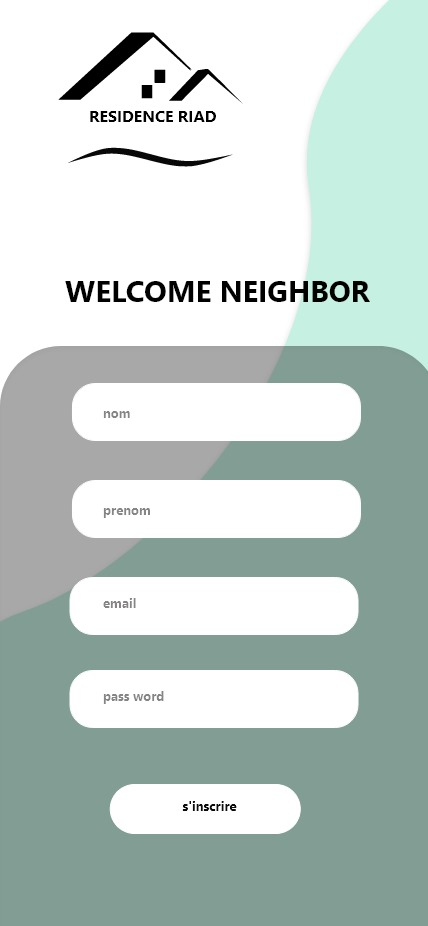
\includegraphics[width=\linewidth]{prototype/signup screen.jpeg}
        \caption{ prototype de l'ecran d'inscription}
  \end{minipage}%
  \begin{minipage}{0.10\textwidth}
    \hfill
  \end{minipage}
\begin{minipage}[t]{0.25\textwidth}
        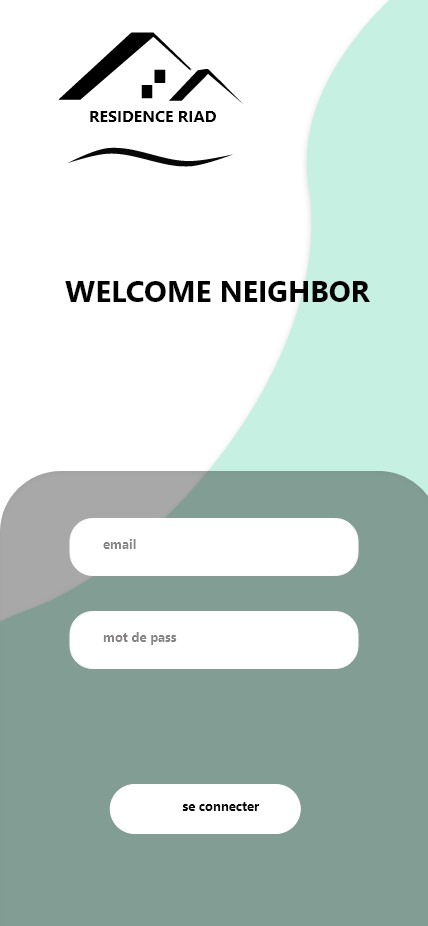
\includegraphics[width=\linewidth]{prototype/sign in.jpeg}
        \caption{ prototype de l'ecran de connexion}
\end{minipage}%
\begin{minipage}{0.10\textwidth}
    \hfill
\end{minipage}
  \begin{minipage}[t]{0.25\textwidth}
        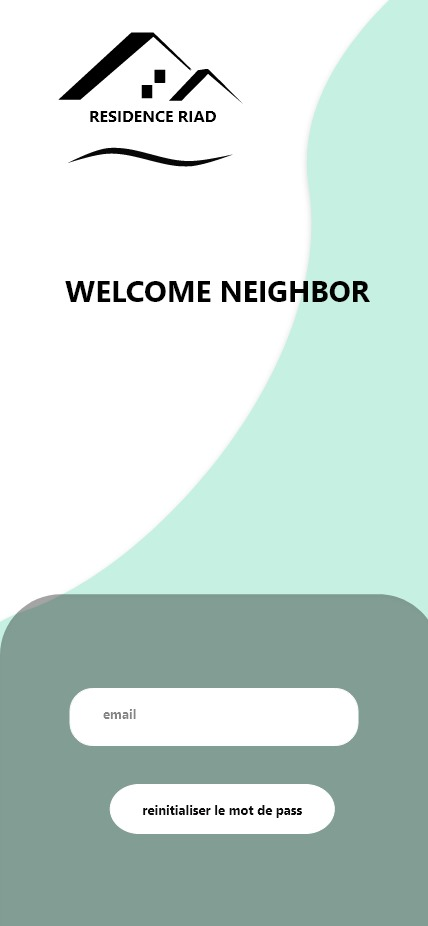
\includegraphics[width=\linewidth]{prototype/reset password.jpeg}
        \caption{ prototype de l'ecran de réinitialisation de mot de passe}
\end{minipage}
\end{figure}
\newpage
\subsubsection{ajout de cotisation et de depenses}
\begin{figure}[h]
    \begin{minipage}[t]{0.25\textwidth}    %% b or t, default is c
            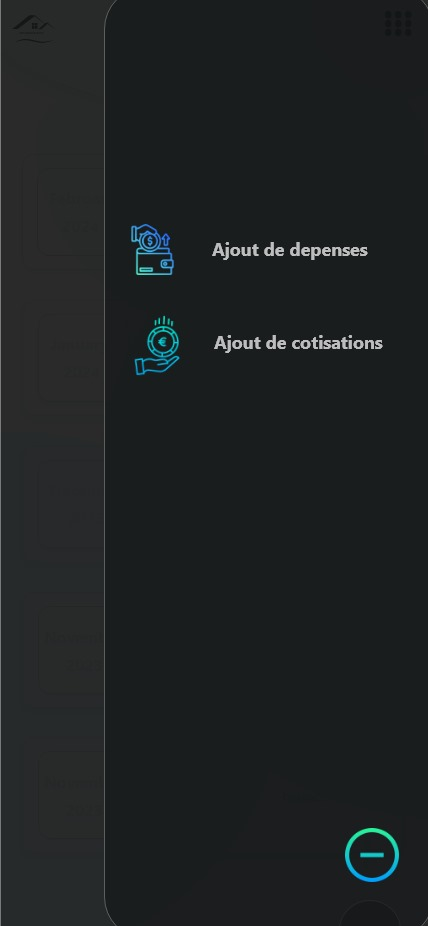
\includegraphics[width=\linewidth]{prototype/side nav.jpeg}
            \caption{ prototype de menu latérale}
      \end{minipage}%
      \begin{minipage}{0.10\textwidth}
        \hfill
      \end{minipage}
    \begin{minipage}[t]{0.25\textwidth}
            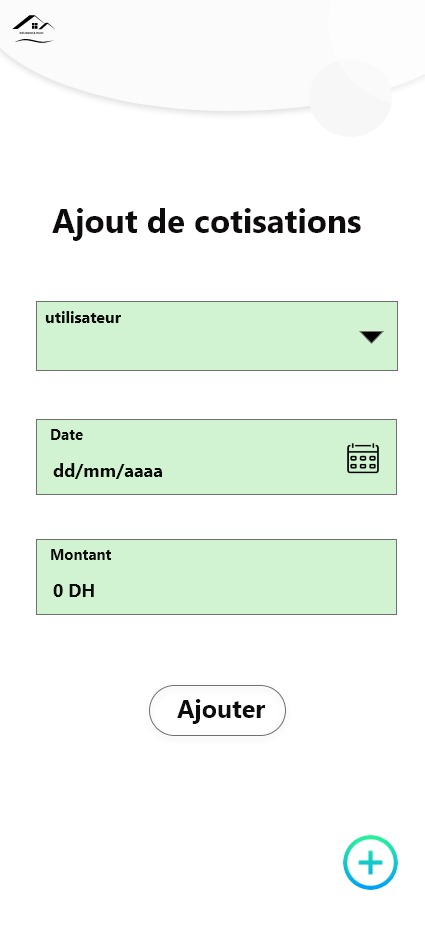
\includegraphics[width=\linewidth]{prototype/add contribution.jpeg}
            \caption{ prototype de l'ecran d'ajout des contributions}
    \end{minipage}%
    \begin{minipage}{0.10\textwidth}
        \hfill
    \end{minipage}
      \begin{minipage}[t]{0.25\textwidth}
            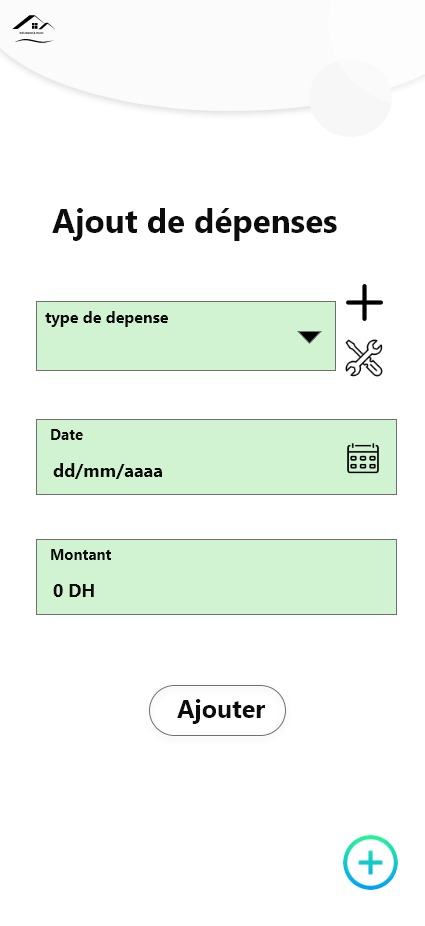
\includegraphics[width=\linewidth]{prototype/add expenses.jpeg}
            \caption{ prototype de l'ecran d'ajout des dépenses}
    \end{minipage}
    \end{figure}
    \newpage
\subsubsection{l'affichage des situations}
\begin{figure}[h!]
    \begin{minipage}[t]{0.25\textwidth}    %% b or t, default is c
            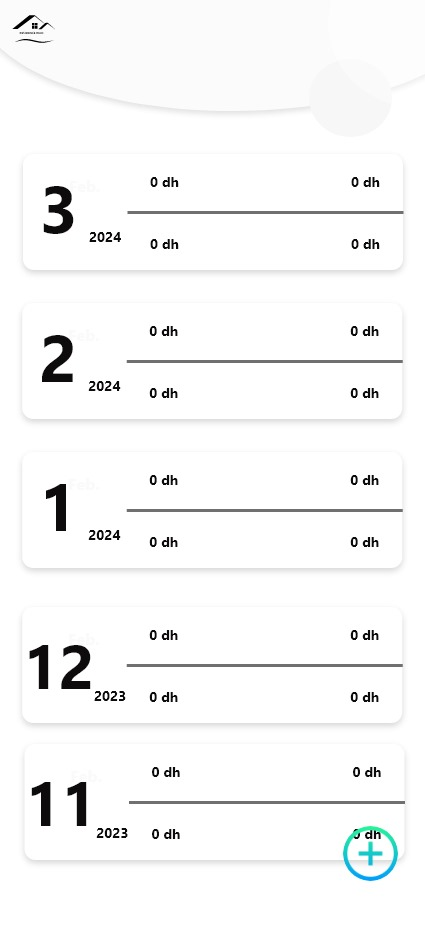
\includegraphics[width=\linewidth]{prototype/admin month view.jpeg}
            \caption{ prototype d'affichage pour l'administrateur}
      \end{minipage}%
      \begin{minipage}{0.10\textwidth}
        \hfill
      \end{minipage}
    \begin{minipage}[t]{0.25\textwidth}
            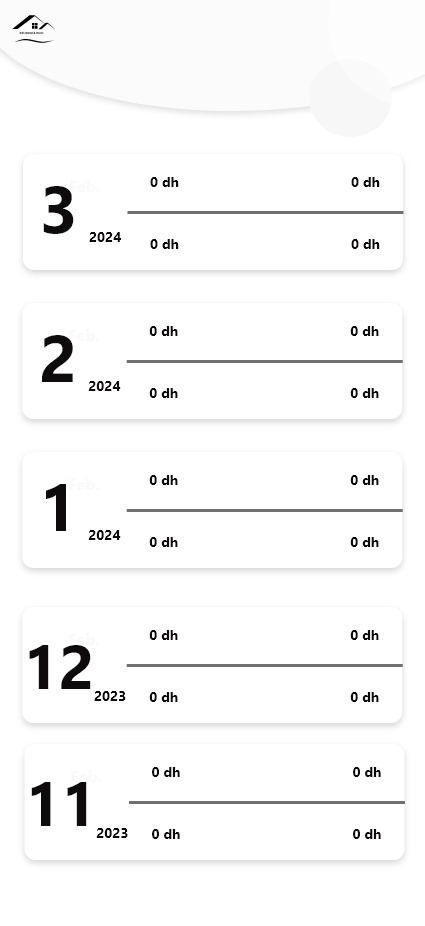
\includegraphics[width=\linewidth]{prototype/user month view.jpeg}
            \caption{ prototype d'affichage pour l'utilisateur}
    \end{minipage}%
    \begin{minipage}{0.10\textwidth}
        \hfill
    \end{minipage}
      \begin{minipage}[t]{0.25\textwidth}
            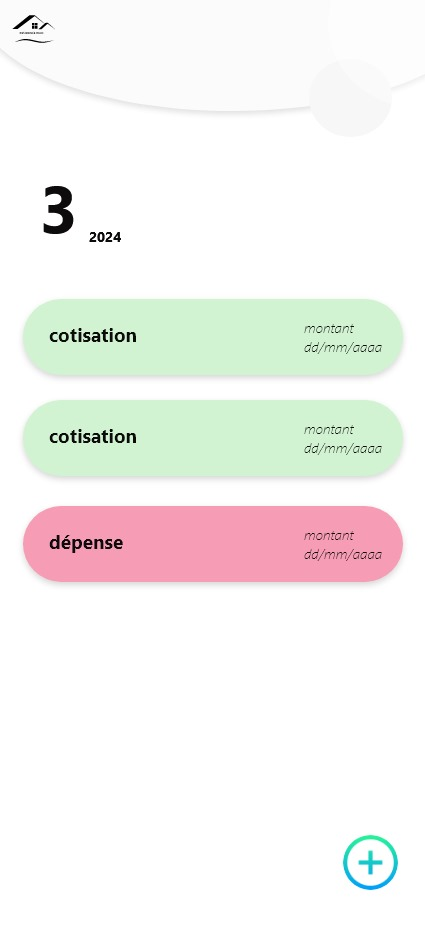
\includegraphics[width=\linewidth]{prototype/month details.jpeg}
            \caption{ prototype d'affichage des opérations}
    \end{minipage}
    \end{figure}
\section{Sprint 1}
\subsection{specification fonctionnel}
\subsubsection{S'inscrire}
Cette opération permet à un utilisateur de créer un nouveau compte dans l'application.
l'utilisateur fournit ses informations personnelles telles que son nom,son prènom, son adresse e-mail et un mot de passe pour créer son compte. après une vérification des informations fournies le nouvel utilisateur sera enregister dans la  base de données.
\subsubsection{Se connecter}
L'opération de connexion permet à un utilisateur enregistré d'accéder à son compte. L'utilisateur saisit son adresse e-mail et son mot de passe dans les champs prévus à cet effet. L'application vérifie les informations saisies et authentifie l'utilisateur si les informations sont correctes
\subsubsection{Réinitialisation le mot de passe}
Cette opération permet à un utilisateur de réinitialiser son mot de passe en cas d'oubli. L'utilisateur fournit son adresse e-mail associée à son compte. L'application envoie un lien de réinitialisation par e-mail à l'utilisateur. L'utilisateur peut ensuite cliquer sur le lien pour choisir un nouveau mot de passe et le mettre à jour dans la base de données.
\subsection{Sprint Backlog}
\begin{center}
    \begin{tabular}{ | m{1cm} | m{9cm}| m{2cm} | m{2cm} |} 
     \hline
     GitHub ID & Sprint Backlog & Acteur & Priorité \\ [0.5ex] 
     \hline\hline
     \#2 & en tant qu'administrateur, je veux avoir la possibilité de m'authentifier en utilisant mon login et mon mot de passe de manière sécurisée afin d'exploiter l'application & Administrateur & ELVEE \\ 
     \hline
     \#3  & En tant qu'utilisateur de l'application, je veux avoir la possibilité de m'authentifier en utilisant mon login et mon mot de passe de manière sécurisée afin d'exploiter l'application & Utilisateur & ELEVEE \\
     \hline
     \#4 & En tant qu'utilisateur, je veux avoir la possibilité de créer un nouveau compte utilisateur afin de l'utiliser & Utilisateur & MOYEN \\
     \hline
     \#5 & En tant qu'utilisateur, je veux avoir la possibilité de réinitialiser mon mot de passe afin de retrouver l'accès a mon compte & Utilisateur & MOYEN \\ [1ex] 
     \hline
    \end{tabular}
\end{center}
\subsection{conception}
Au cours de la phase initiale de conception du premier Sprint, nous avons choisi de focaliser notre attention sur les user stories liées à l'authentification. Les exigences se concentrent sur la possibilité de se connecter à l'application en utilisant un identifiant et un mot de passe, ainsi que sur la capacité de créer un compte et de réinitialiser le mot de passe en cas de besoin.
\subsubsection{diagramme de cas d'utilisation}
D'après les Sprint Backlogs sélectionnés, nous observons la présence de deux acteurs principaux : l'utilisateur et l'administrateur. Ces deux acteurs ont besoin de se connecter via un identifiant et un mot de passe. De plus, ils doivent tous deux avoir la capacité de réinitialiser le mot de passe. Seul l'utilisateur aura le droit de s'inscrire.
\begin{figure}[h!]
    \begin{center}
    \begin{tikzpicture}
        \begin{umlsystem}[x=3, fill=red!10]{Sprint1}
            \umlusecase[name = CONNECT]{se connecter}
            \umlusecase[name = SIGNUP, y = -2]{s'inscrire}
            \umlusecase[name = renewPassword, y = -4]{réinitialiser le mot de passe} 
            \umlusecase[name = AUTH,x = 5,y = -1]{s'authentifier}  
            \end{umlsystem}
        
            \umlactor[x=-2]{utilisateur}
            \umlactor[x =-2,y=-3]{administrateur}
        
        \umlassoc{utilisateur}{CONNECT}
        \umlassoc{utilisateur}{SIGNUP}
        \umlassoc{utilisateur}{renewPassword}
        \umlassoc{administrateur}{CONNECT}
        \umlassoc{administrateur}{renewPassword}

        \umlHVinclude[name=incl]{CONNECT}{AUTH}
       % \umlHVinclude[name=incl]{addSpending}{auth}
        %\umlHVinclude[name=incl,anchor1=30 , anchor2=300]{addBudget}{auth}

    \end{tikzpicture}
    \caption{Le diagramme de cas d'utilisation pour Sprint 1}
\end{center}
    \label{fig : Sprint 1 usecase }
\end{figure}

%and this is a reference to the usecase fig : \ref{fig : usecase 1}

\newpage
\subsubsection{diagramme de classe}
basé sur les meilleures pratiques citées ci-dessous, nous avons opté pour le modèle MVVM. Nous avons dû créer 3 vues pour : 
\begin{itemize}
  \item la connexion;
  \item l'inscription;
  \item la réinitialisation du mot de passe. 
\end{itemize}
Ces vues ont été créées en utilisant Jetpack Compose, un framework d'interface utilisateur déclaratif basé sur des fonctions plutôt que sur des classes Activity ou les anciens fichiers XML, ce qui explique pourquoi les vues ne sont pas mentionnées dans le diagramme de classes.

Pour le modèle, nous avons dû créer un modèle pour l'utilisateur; une classe contenant une variable booléenne décrivant s'il s'agit d'un administrateur ou non, et plusieurs variables de type chaîne de caractère contenant le nom, le nom de famille, l'identifiant et l'e-mail.

Pour le viewModel : nous avons opté pour un ViewModel unifié car cela n'est pas au contraire des meilleures pratiques et pour simplifier la base de code.

La classe authViewModel est une classe qui hérite de la classe ViewModel et contient 3 valeurs mutableState utilisées pour mettre à jour les interfaces graphiques de chaque vue : LoginUiState, registerUiState, resetUiState pour les vues de connexion, d'inscription et de réinitialisation respectivement.

Le viewModel contient également une valeur accountService injectée lors de la création du viewModel (en utilisant le constructeur) grâce à Dagger-Hilt Dependency Injector.

Le accountService est une interface où nous avons déclaré toutes les fonctions nécessaires.
Nous avons créé une autre classe qui étend cette interface appelée FireBaseAccountService afin de faciliter le support d'autres backends.

Dans le AuthViewModel, nous avons implémenté toutes les fonctions nécessaires appelées par les vues. Par exemple : login est une fonction appelé lorsque l'utilisateur clique sur le bouton  <<connexion>>. Il récupère l'e-mail et le mot de passe à partir de LoginUIState, puis les passe ces parametres et appelle la méthode authenticate de l'instance FireBaseAccountService.

Pour personnaliser les messages d'erreur de SnackBar, nous avons dû créer nos propres exceptions,la classe AuthException. Toutes sortes d'exceptions survenues lors de l'authentification sont des exceptions spécifiques à Firebase qui sont converties en exceptions héritées de AuthException. Ensuite, ces exceptions sont gérées par la fonction loginExceptionHandler du AuthViewModel, qui récupère simplement le message de l'exception et l'affiche à l'aide d'un SnackBar.
\begin{figure}[h!]
        \begin{tikzpicture}
        
        \umlclass[x=0,y=0,type=interface,scale = 0.55,fill=blue!10]{AccountService}{
          }{ 
            + authenticate (login : LoginUiModel, onResult: (User) -> Unit) :Unit\\
            + logout() : Unit \\
            + Register(Register: RegisterUiModel, onResult: (User) -> Unit) : Unit \\
            + reset(email: String,onResult: () -> Unit) : Unit \\
          }
          \umlclass[x=9,y=0,scale = 0.55,fill=blue!10]{FireBaseAccountService}{
          }{ 
            - resetPasswordListener(task: Task<Void>, onResult: () -> Unit) :Unit\\
            - loginListerner(task: Task<AuthResult>,onResult: (User) -> Unit) : Unit \\
            - registerListerner(t:Task<AuthResult>,r:RegisterUiModel,onResult:(User)->Unit) :Unit \\
            - setUserData(t:Task<AuthResult>,u:String?,r:RegisterUiModel,onResult:(User)->Unit) : Unit \\
            - authException(e:Exception) :AuthException\\
            - getUserData(task:Task<AuthResult>,uid:String?,onResult:(User) -> Unit) :Unit\\
            - ongetUserDataSucessListener(document: DocumentSnapshot,onResult: (User) -> Unit) :Unit\\
            - onFirestoreException(e: java.lang.Exception) :Unit\\
          }
          \umlclass[x=1,y=-3,scale = 0.55,,fill=green!10]{RegisterUiModel}{
            + prenom : String \\
            + nom : String \\
            + email : String \\
            + password : String
          }{}
            \umlclass[x=-2,y=-3,scale = 0.55,fill=green!10]{LoginUiModel}{
            + email : String \\
            + password : String
          }{}
              \umlclass[x=1,y=-6,scale = 0.55,fill=orange!10]{LoginUiState}{
            + email : String \\
            + password : String \\
            + logging : Boolean \\
            + validMail : Boolean
          }{}
              \umlclass[x=4,y=-6,scale = 0.55,fill=orange!10]{ResetUiState}{
            + email : String \\
            + isMailValid : Boolean
          }{}
          
              \umlclass[x=-2,y=-6,scale = 0.55,fill=orange!10]{RegisterUiState}{
            + prenom : String \\
            + nom : String \\
            + email : String \\
            + password : String \\
            + validMail : Boolean
          }{}
        
          \umlclass[x=8,y=-3,scale = 0.55,fill=red!10]{Exception}{
          }{
          } 
          
          \umlclass[x=8,y=-5,type=abstract,scale = 0.55,fill=red!10]{AuthException}{
          }{
            + getmessage() : Int
          }
            \umlclass[x=12,y=-3,scale = 0.55,fill=red!10]{DeadLineExceeded}{
          }{
          }
             \umlclass[x=12,y=-4,scale = 0.55,fill=red!10]{InvalidCredentialsException}{
          }{
          }
        
           \umlclass[x=12,y=-5,scale = 0.55,fill=red!10]{InvalidUserIdException}{
          }{
          }
        
          \umlclass[x=12,y=-6,scale = 0.55,fill=red!10]{MalFormatedEmailException}{
          }{
          }
        
            \umlclass[x=12,y=-7,scale = 0.55,fill=red!10]{RegisterPasswordMismatchException}{
          }{
          }
        
              \umlclass[x=12,y=-8,scale = 0.55,fill=red!10]{UndefinedException}{
          }{
          } 
        
          \umlclass[x=12,y=-9,scale = 0.55,fill=red!10]{UserDataMissingException}{
          }{
          } 
        
            \umlclass[x=4,y=-3,scale = 0.55,fill=white!10]{User}{
            - IS\_ADMIN:Boolean \\
            name : String \\
            familyname : String \\
            id : String \\
            email : String
          }{
          } 
        \umlclass[x=8,y=-7,scale = 0.55,fill=yellow!10]{ViewModel}{
          }{
          } 
        
        \umlclass[x=4,y=-11,scale = 0.55,fill=yellow!10]{AuthViewModel}{
            + loginUistate :  MutableState<LoginUiState> \\
            + registerUistate : MutableState<RegisterUiState> \\
            + resetUiState : MutableState<ResetUiState> \\
          }{
            +Constructor(accountService : AccountService) \\ % TODO: find the correct way to represent the constructor
            + login(openAndPopUp:(String,String)->Unit,toggleAdminUservalues:(isadmin:Boolean,logged:Boolean)->Unit)  : Unit \\
            + loginExceptionHandler(e: AuthException) : Unit \\
            + setUser(user: User) : Unit \\
            + signupscreen(open: ( String) -> Unit) : Unit \\
            + setLoginEmail(newemail:String) : Unit \\
            + setLoginPassword(newpass:String) : Unit \\
            + onLoginEmailValidation(valid: Boolean) :  Unit \\
            + register(openAndPopUp: (String, String) -> Unit) : Unit \\
            + setRegisterName(s: String) : Unit \\
            + setFamilyname(s: String) : Unit \\
            + setEmail(s: String) : Unit \\
            + setRegisterPass(s: String) : Unit \\
            + setVerificationPass(s: String) : Unit \\
            + onRegisterEmailValidation(valid: Boolean) : Unit \\
            + resetSetEmail(s: String) : Unit \\
            + resetPassword(openAndPopUp: (String, String) -> Unit) : Unit \\
            + onResetEmailValidation(b: Boolean) : Unit \\
            + resetPasswordScreen(open: (String) -> Unit) : Unit 
          } 
        
        \umlinherit{AuthViewModel}{ViewModel}
        \umlinherit{FireBaseAccountService}{AccountService}
        \umlinherit{AuthException}{Exception}
        \umlinherit{DeadLineExceeded}{AuthException}
        \umlinherit{InvalidCredentialsException}{AuthException}
        \umlinherit{InvalidUserIdException}{AuthException}
        \umlinherit{MalFormatedEmailException}{AuthException}
        \umlinherit{RegisterPasswordMismatchException}{AuthException}
        \umlinherit{UndefinedException}{AuthException}
        \umlinherit{UserDataMissingException}{AuthException}
        
        \umlaggreg[]{AuthViewModel}{LoginUiState}
        \umlaggreg[]{AuthViewModel}{RegisterUiState}
        \umlaggreg[]{AuthViewModel}{ResetUiState}
        
        \umlassoc[]{User}{AccountService}
        \umlassoc[]{AuthException}{AuthViewModel}
        \umlassoc[]{User}{AuthViewModel}
        \umlassoc[]{LoginUiModel}{AuthViewModel}
        \umlassoc[]{RegisterUiModel}{AuthViewModel}
        \umlassoc [geometry=|-, anchors=-160 and 170,] {AccountService}{AuthViewModel}
        
        %\umlunicompo[geometry=-|, arg=titi, mult=*, pos=1.7, stereo=vector]{D}{C}
        %\umlimport[geometry=|-, anchors=90 and 50, name=import]{sp2}{sp1}
        %\umlinherit[geometry=-|]{D}{B}
        \end{tikzpicture}
        \caption{le diagramme de Class pour Sprint 1}
        \label{fig : Class diagram Sprint 1}
    \end{figure}
\subsection{Realisation}
\subsubsection{interface de connexion}
\begin{figure}[!htbp]
  \begin{minipage}[t]{0.4\textwidth}    %% b or t, default is c
          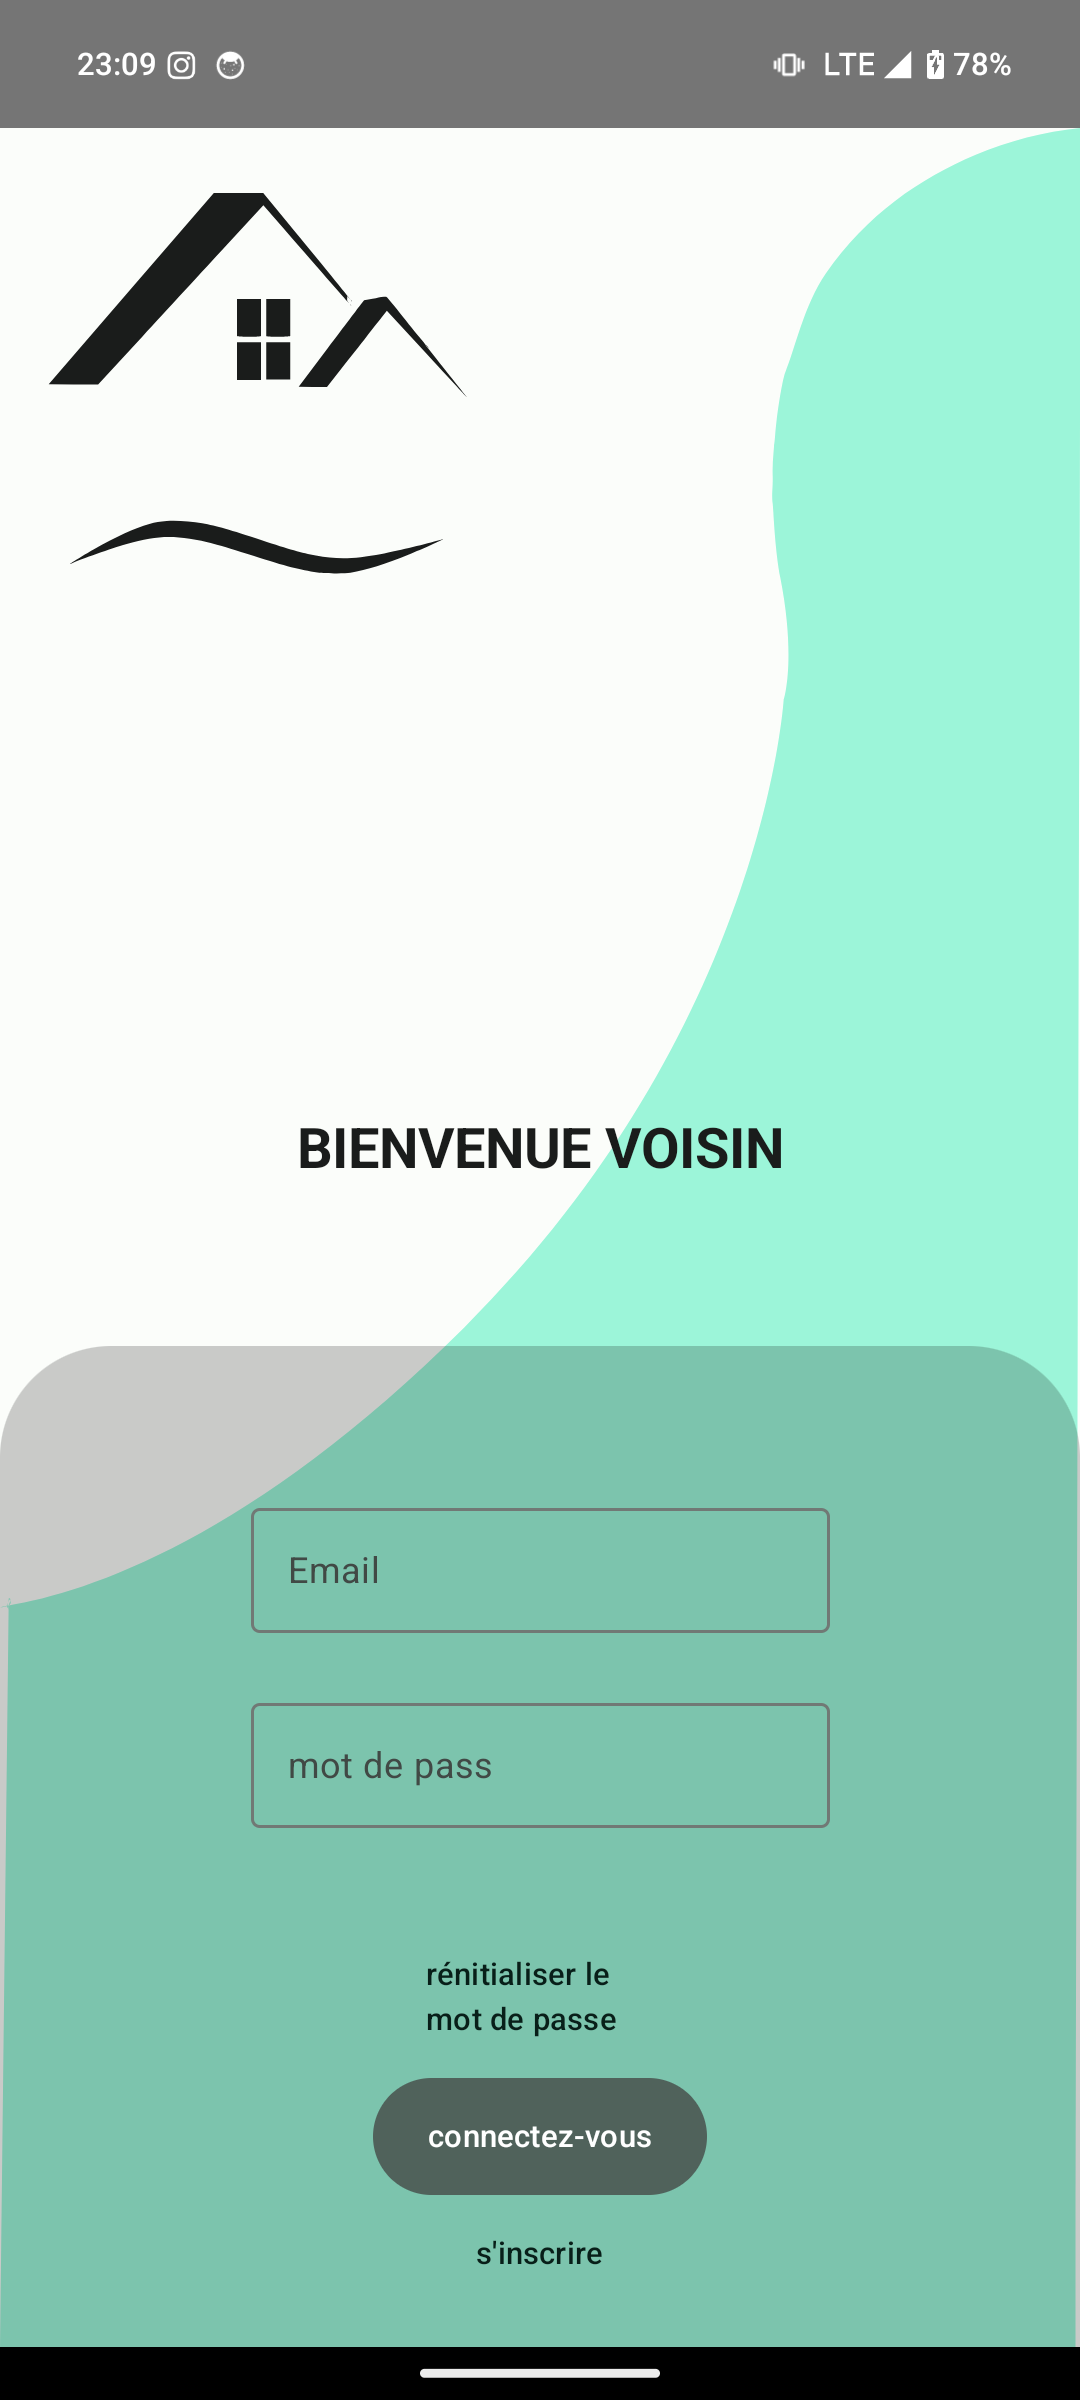
\includegraphics[width=\linewidth]{Screenshots/8.png}
          \caption{ ecran de connexion (light mode)}
  \end{minipage}%
    \begin{minipage}{0.20\textwidth}
      \hfill
    \end{minipage}
  \begin{minipage}[t]{0.4\textwidth}
          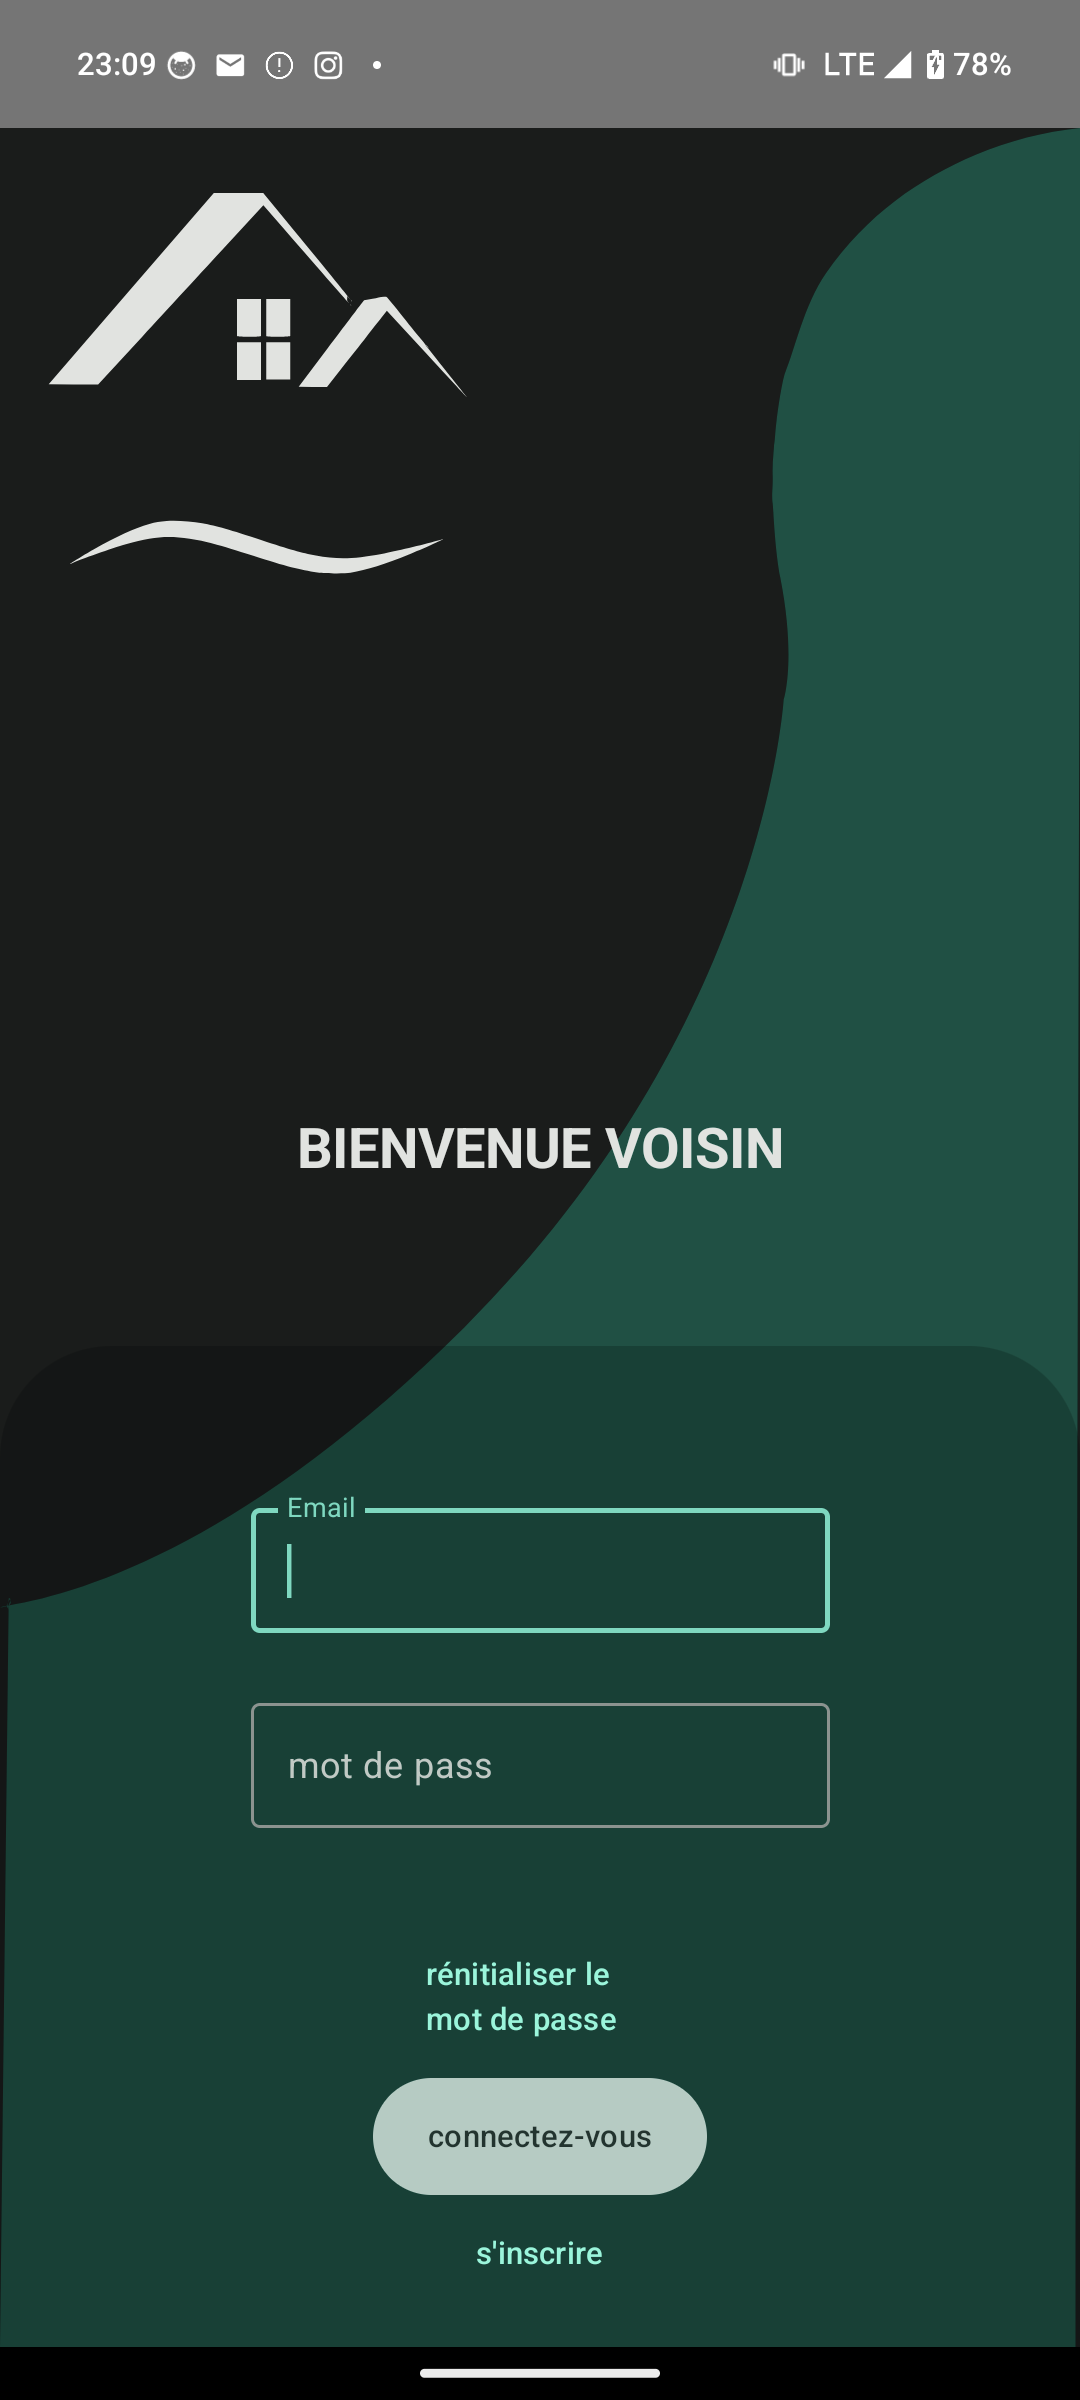
\includegraphics[width=\linewidth]{Screenshots/7.png}
          \caption{ ecran de connexion (dark mode)}
  \end{minipage}%
  \end{figure}
  \hfill
  $ $
  \subsubsection{interface d'inscription et de renitialisation de mot de passe}
  $ $
  \begin{figure}[!htbp]
    \begin{minipage}[t]{0.4\textwidth}    %% b or t, default is c
            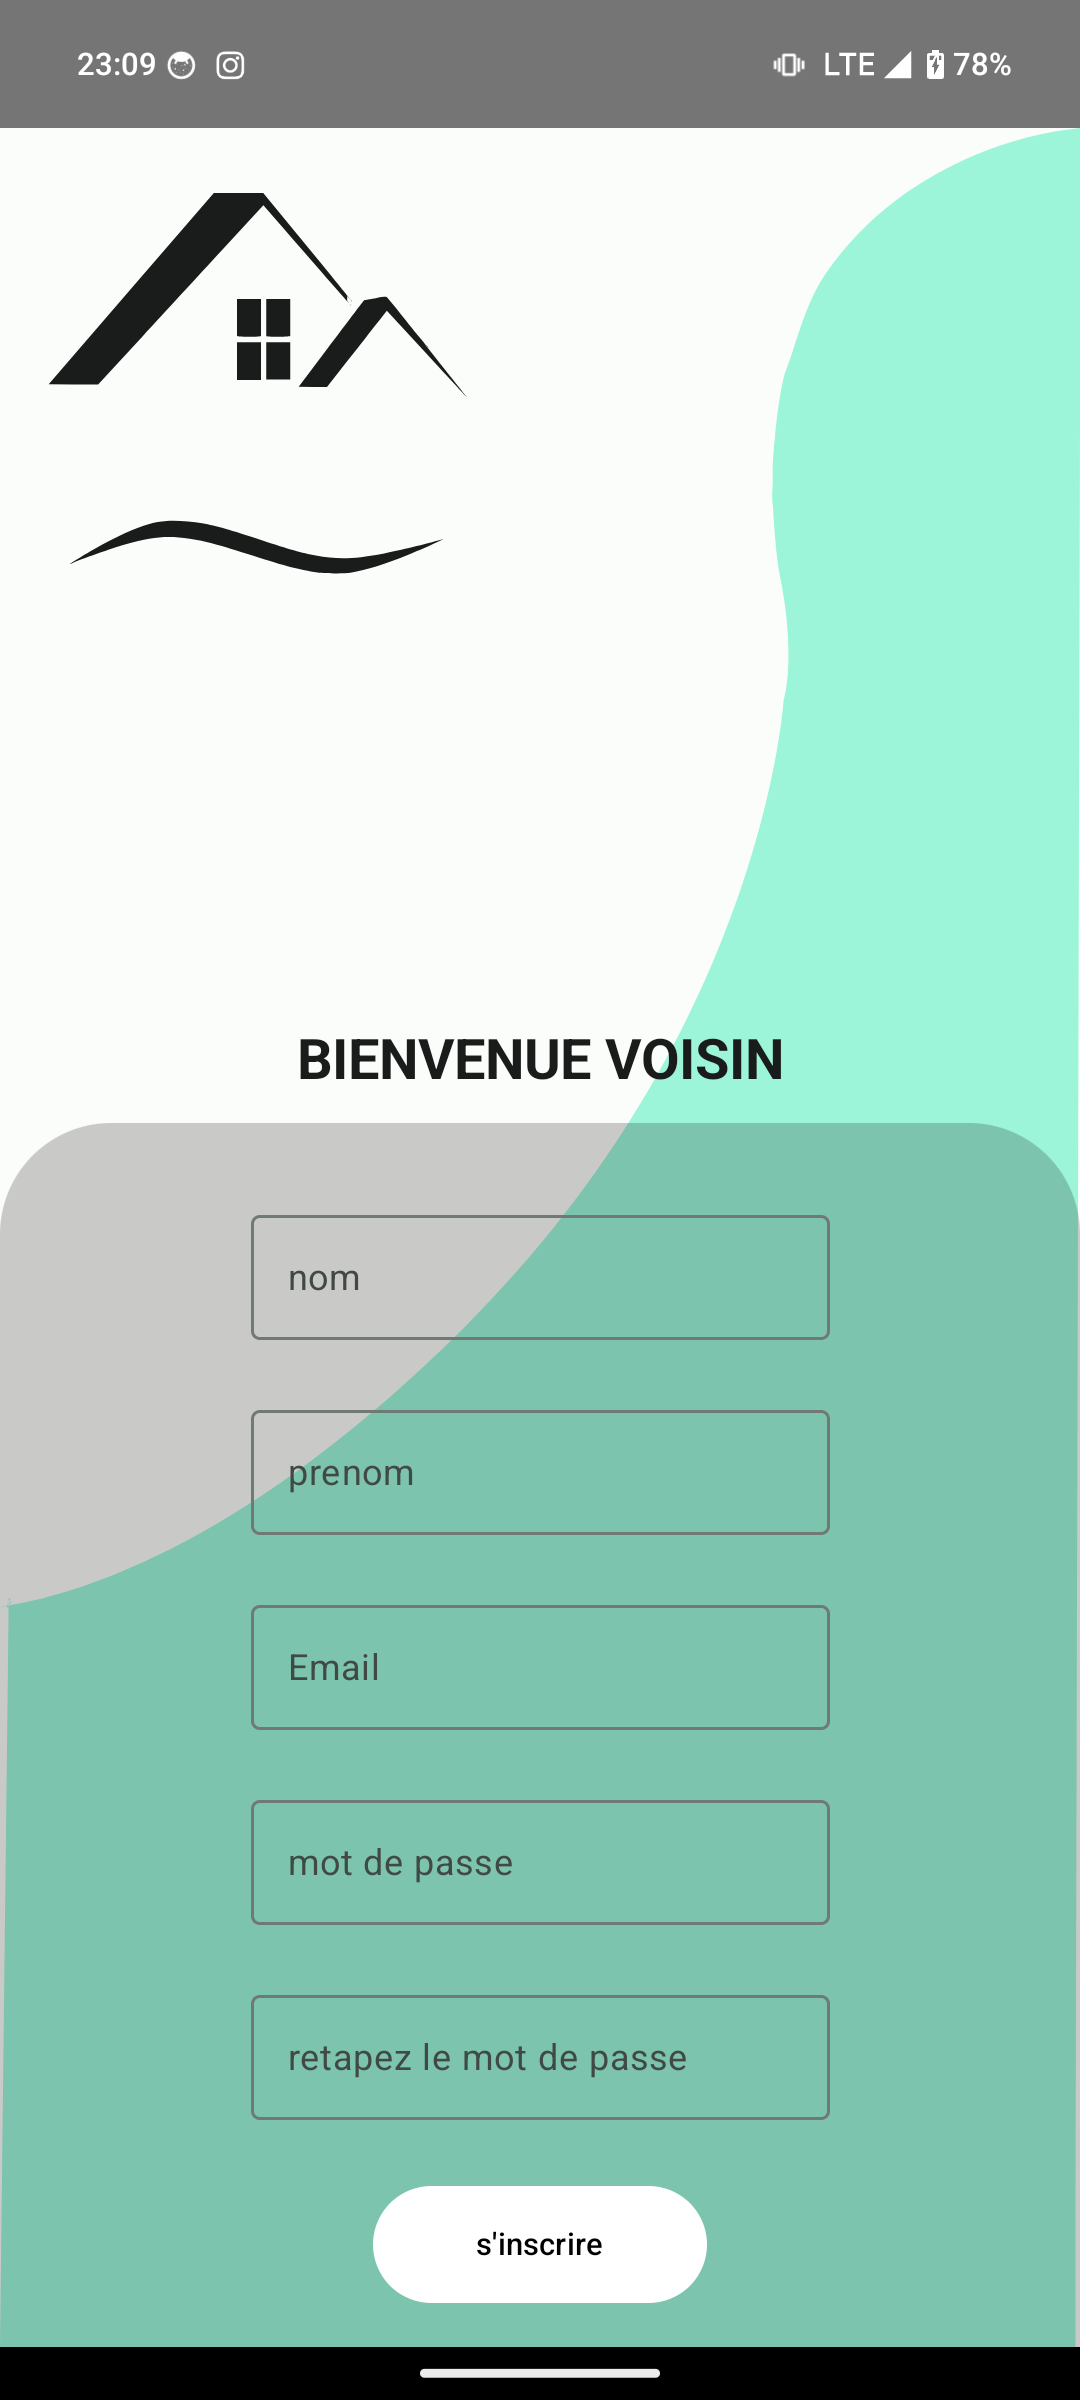
\includegraphics[width=\linewidth]{Screenshots/10.png}
            \caption{ ecran d'inscription}
    \end{minipage}%
    \begin{minipage}{0.20\textwidth}
      \hfill
    \end{minipage}
  \begin{minipage}[t]{0.4\textwidth}
          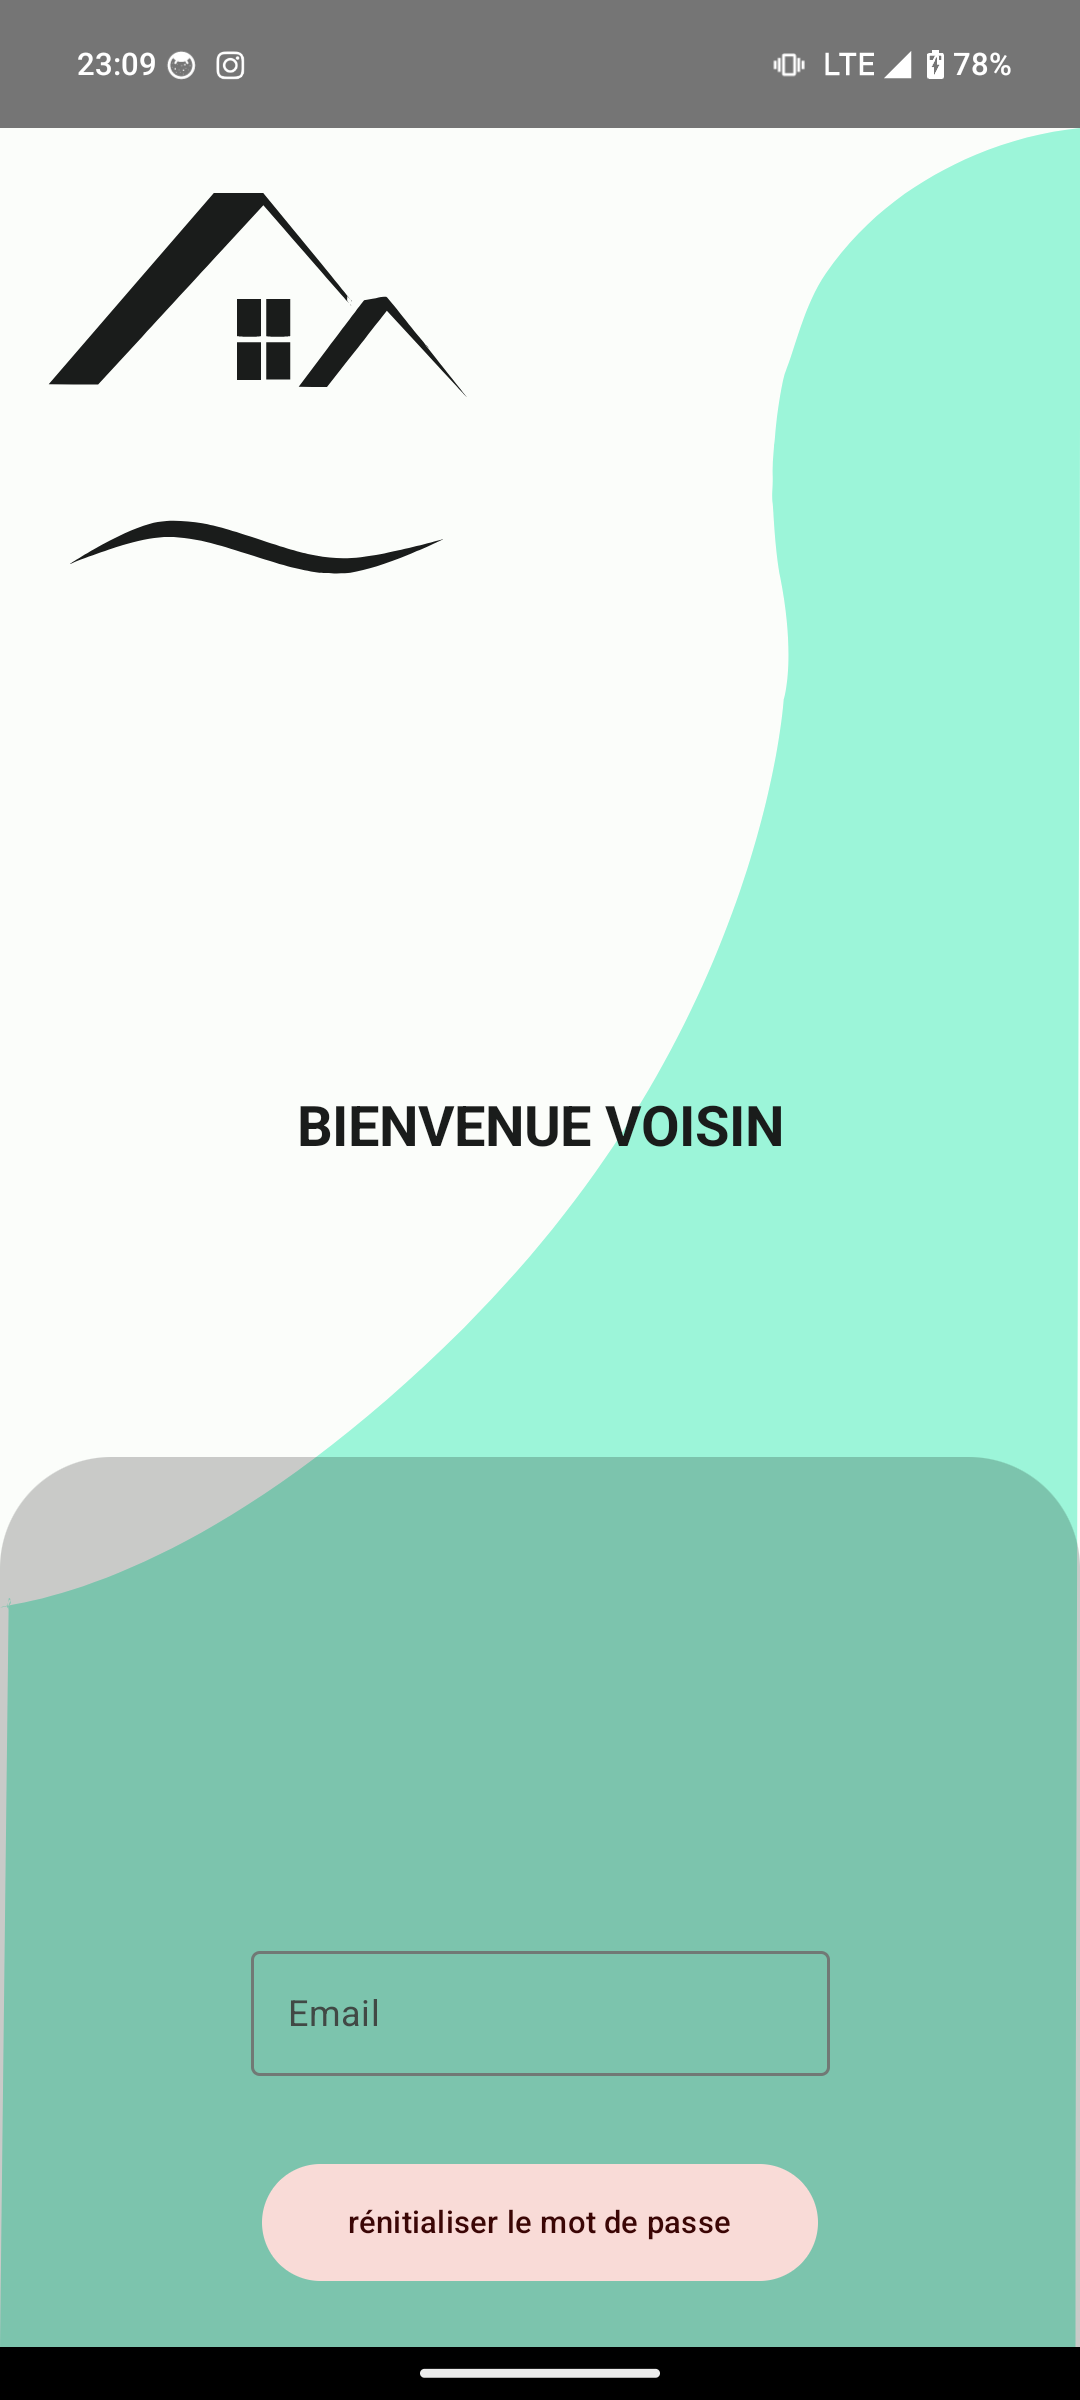
\includegraphics[width=\linewidth]{Screenshots/9.png}
          \caption{ ecran de reinitialisation de mot de passe}
  \end{minipage}%
    \end{figure}
\begin{figure}[!htbp]
      \begin{minipage}[t]{0.4\textwidth}    %% b or t, default is c
              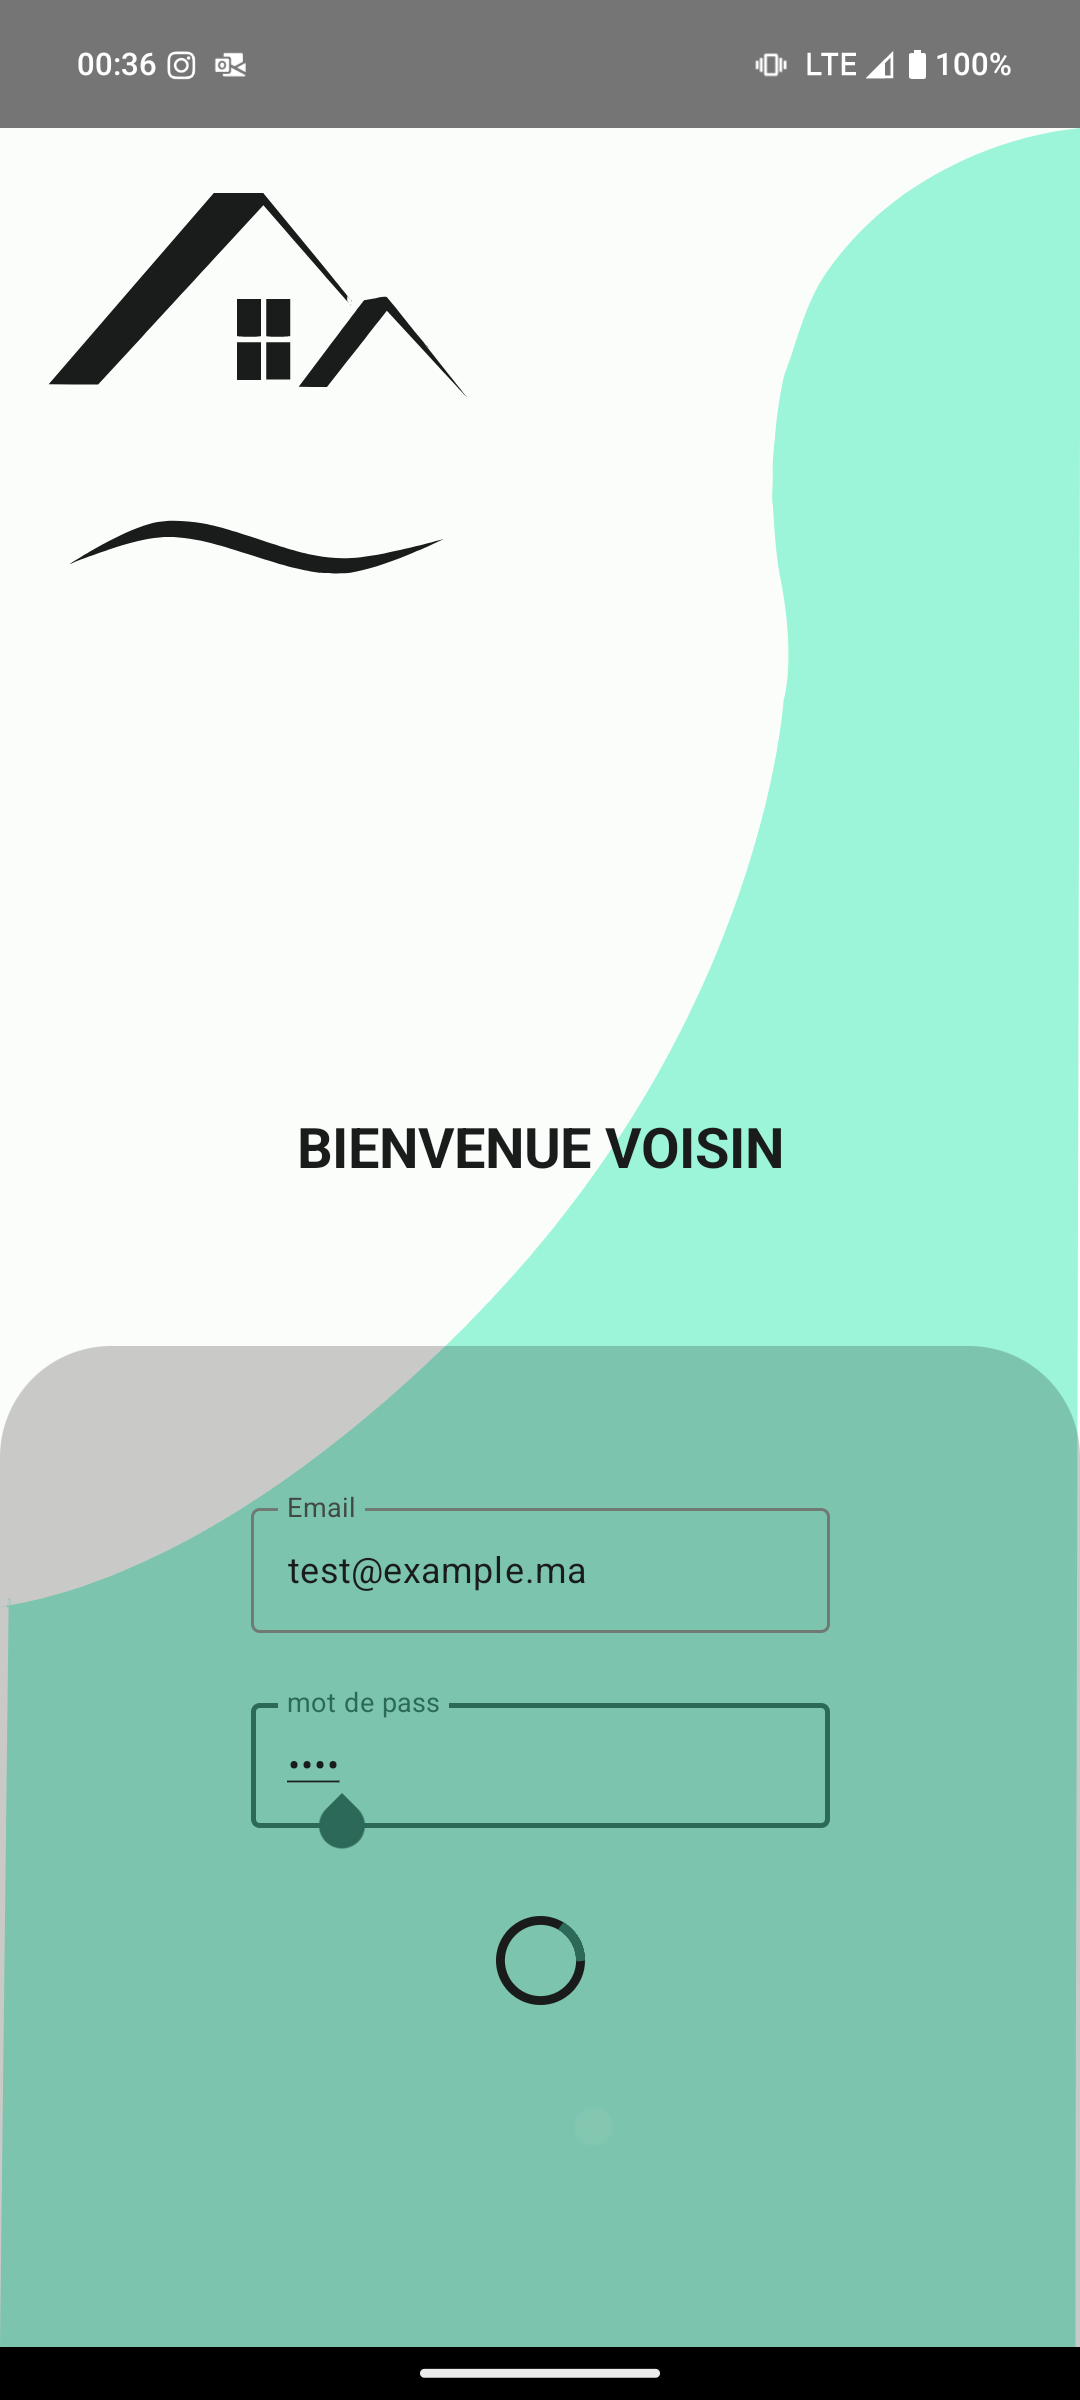
\includegraphics[width=\linewidth]{Screenshots/b4.png}
              \caption{ animation lors de connexion}
      \end{minipage}%
      \begin{minipage}{0.20\textwidth}
        \hfill
      \end{minipage}
    \begin{minipage}[t]{0.4\textwidth}
            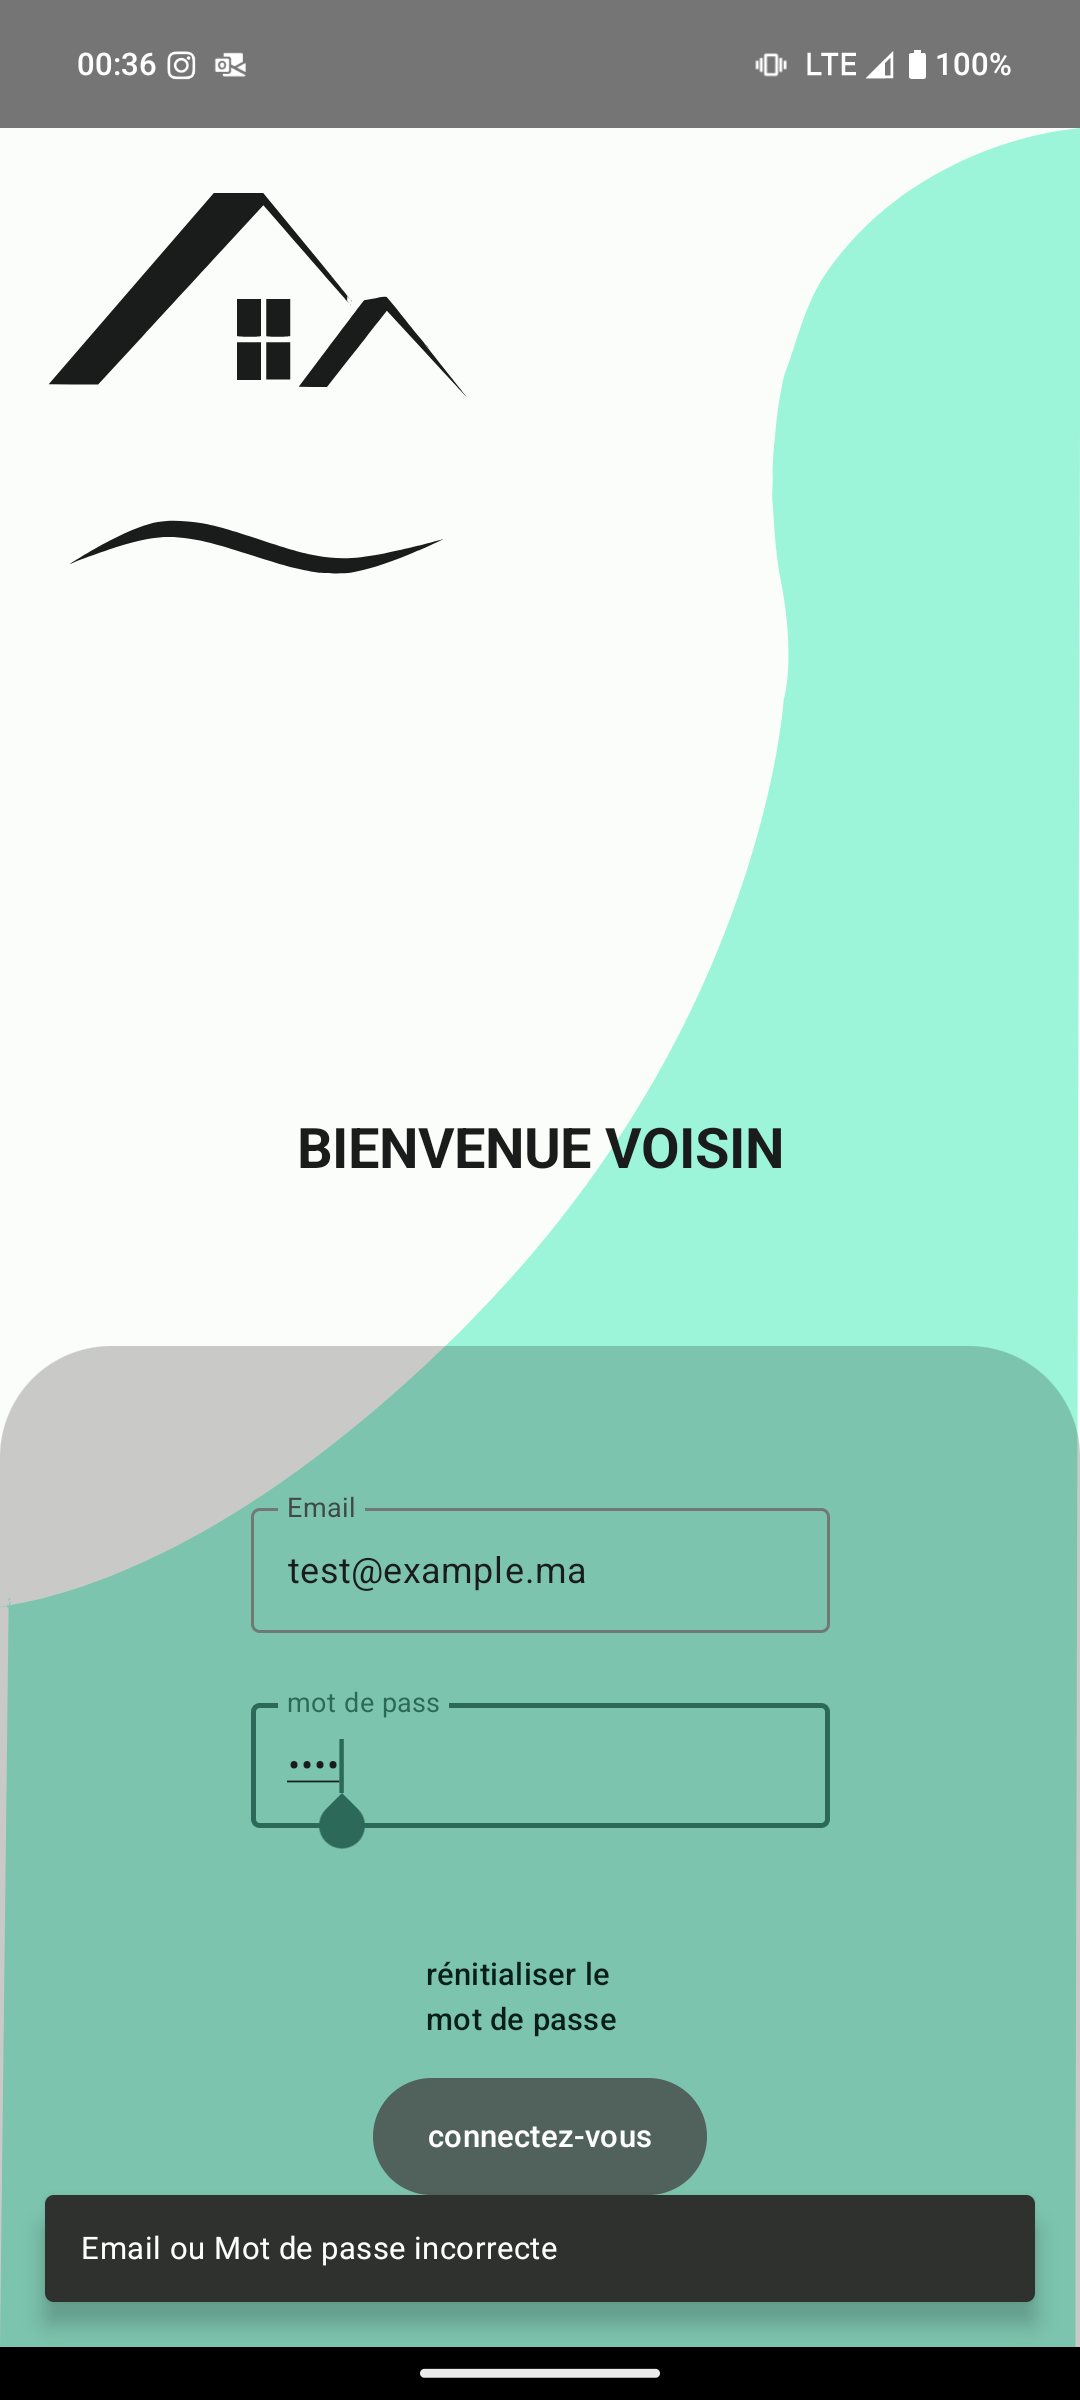
\includegraphics[width=\linewidth]{Screenshots/b2.png}
            \caption{ exemple d'erreur 1}
    \end{minipage}%
      \end{figure}
      \begin{figure}[!htbp]
        \begin{minipage}[t]{0.4\textwidth}    %% b or t, default is c
                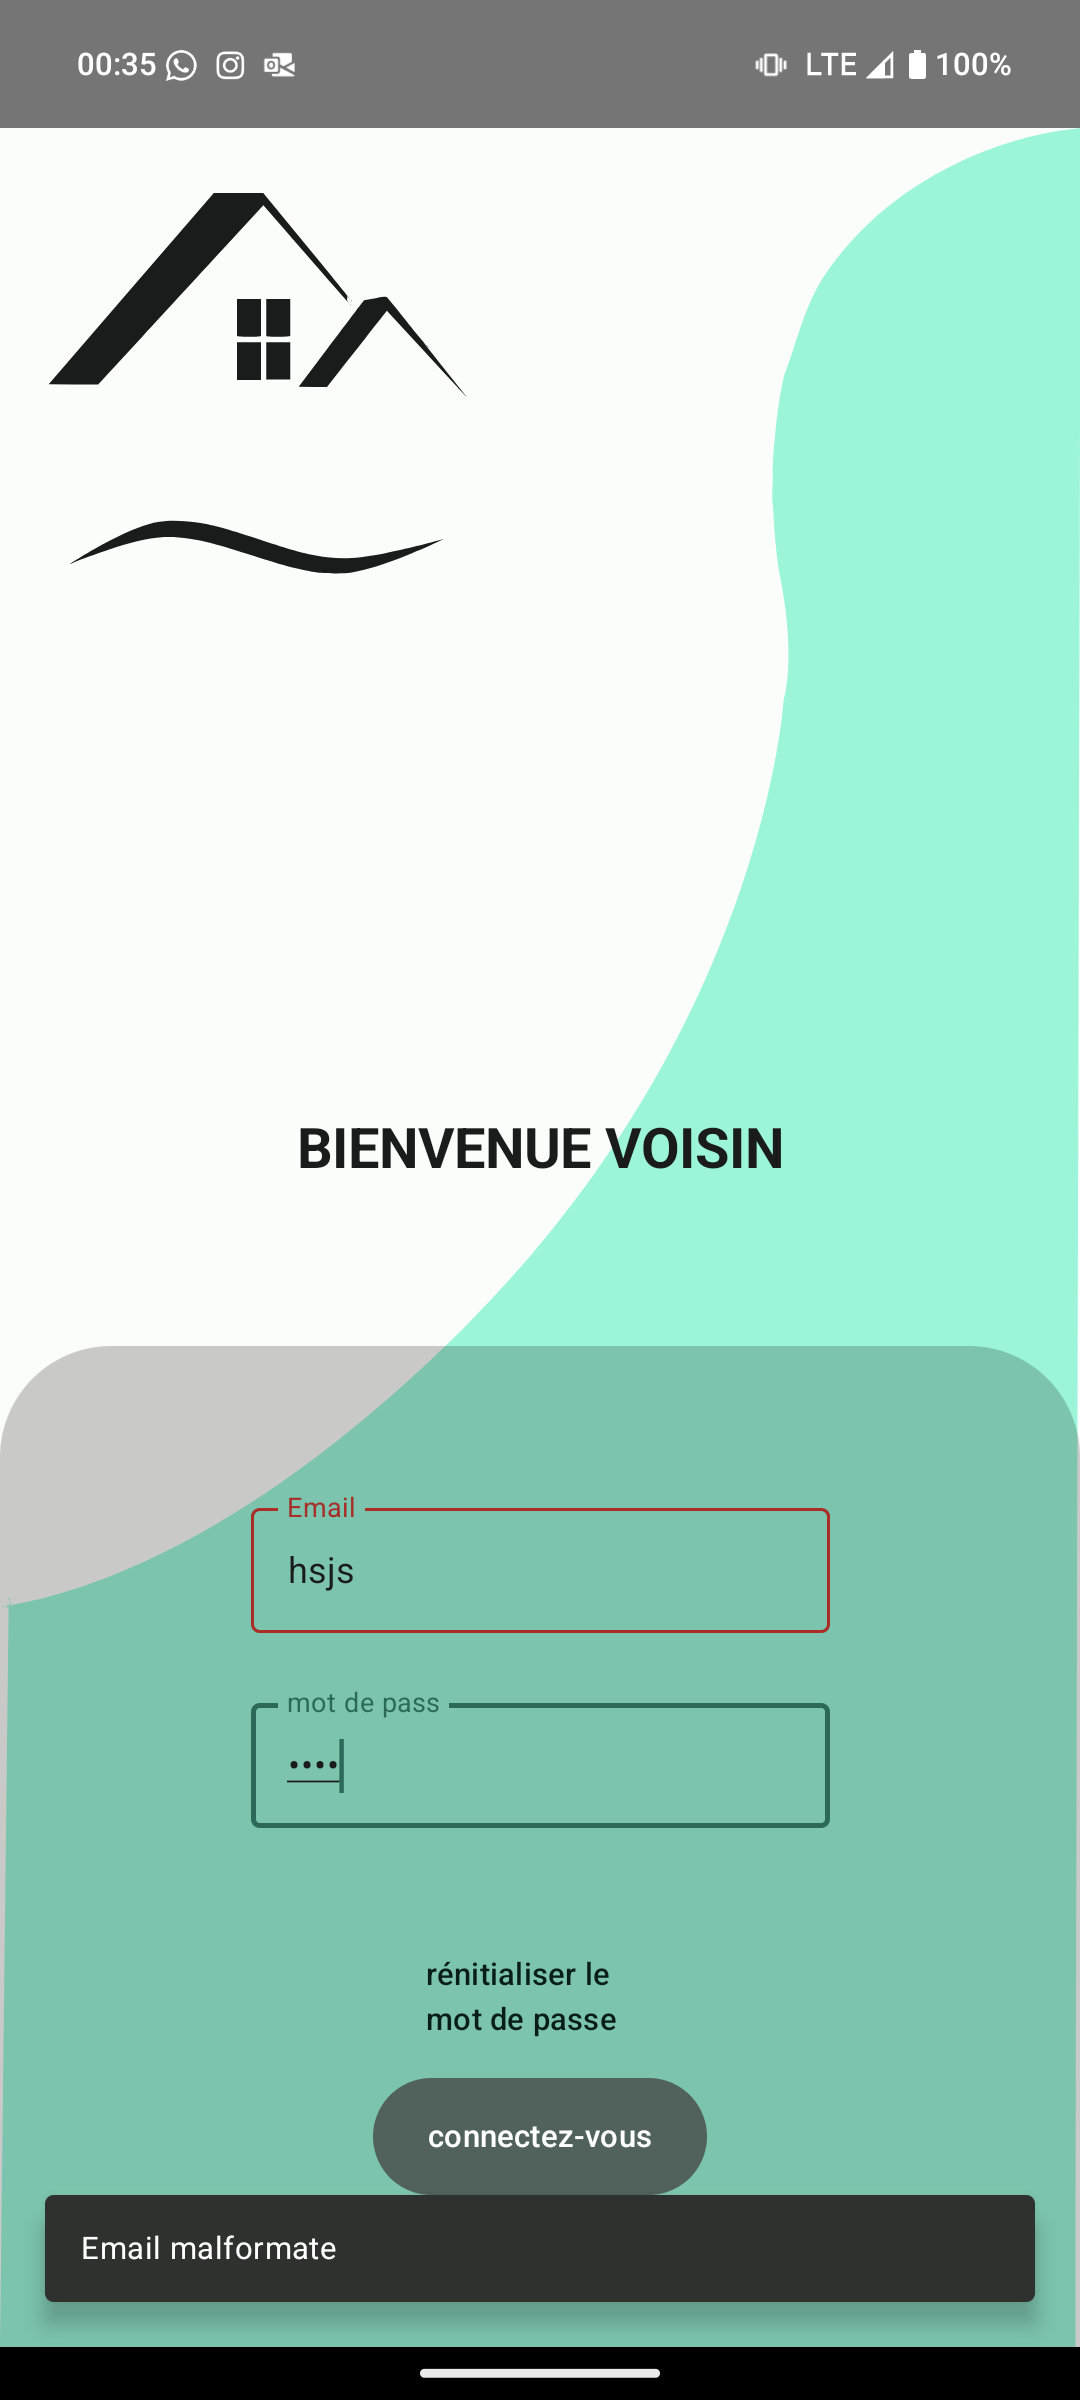
\includegraphics[width=\linewidth]{Screenshots/b1.png}
                \caption{ exemple d'erreur 2}
        \end{minipage}%
        \begin{minipage}{0.20\textwidth} 
          \hfill
        \end{minipage}
      \begin{minipage}[t]{0.4\textwidth}
              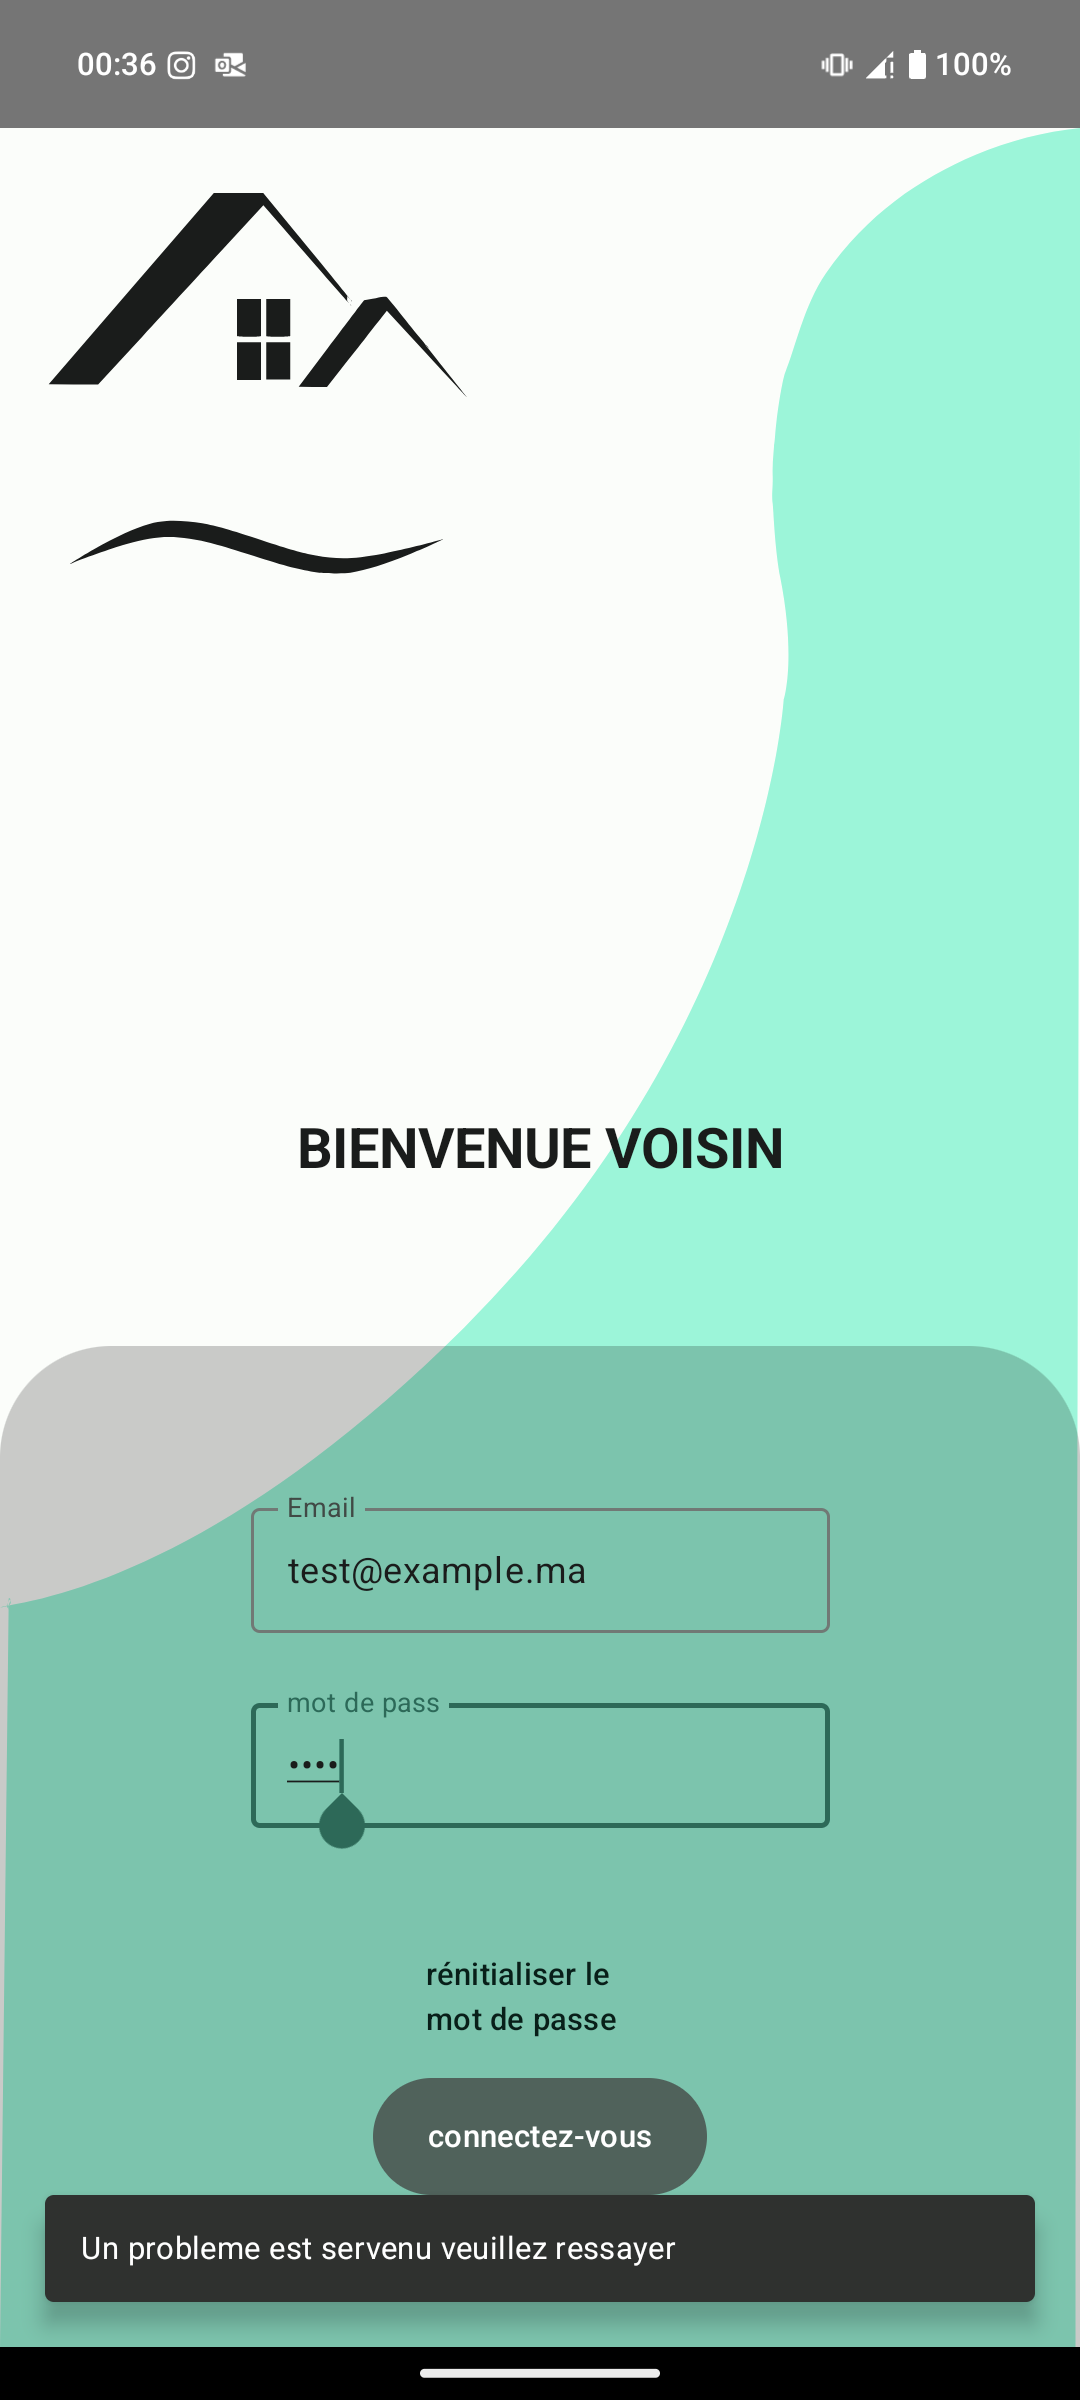
\includegraphics[width=\linewidth]{Screenshots/b3.png}
              \caption{ exemple d'erreur 3}
      \end{minipage}%
        \end{figure}
\newpage
\section{Sprint 2}
\subsection{specification fonctionnel}
\subsubsection{consulter la situation des mois}
Cette fonctionnalité permet à l'utilisateur de visualiser la liste des mois disponibles, avec les données associées à chaque mois telles que les revenus, les dépenses et le solde. Ces informations peuvent aider l'utilisateur à suivre les finances mois par mois et à avoir une vue d'ensemble des finances sur une période donnée.
\subsubsection{consulter les operations de chaque mois}
Cette fonctionnalité offre à l'utilisateur la possibilité de consulter en détail les revenus et les dépenses par mois.une liste des operations serait affiché en precisant la date de l'operation et montant d'operation, le cotisateur s'il s'agit d'une cotisation ou le type de depense s'il s'agit d'une depense.

\subsection{Sprint Backlog}
\begin{center}
  \begin{tabular}{ | m{1cm} | m{9cm}| m{2cm} | m{2cm} |} 
   \hline
   GitHub ID & Sprint Backlog & Acteur & Priorité \\ [0.5ex] 
   \hline\hline
   \#23 & en tant qu'utilisatuer, je veux voir les revenus, les dépenses, et le solde de chaque mois afin de mieux saisir la situation & Utilisateur & ELEVEE \\ 
   \hline
   \#24  & En tant qu'utilisateur je veux voir en détail les dépenses et les revenus par mois afin de mieux saisir la situation de chaque mois, & Utilisateur & ELEVEE \\
   \hline
  \end{tabular}
\end{center}
\subsection{conception}
Dans le deuxième Sprint, nous avons décidé de nous attaquer aux backlogs liés à la visualisation des données. Les besoins sont les suivants : montrer la situation globale et présenter une situation spécifique pour chaque mois.
\subsubsection{diagramme de cas d'utilisation}
Nous allons conserver nos principaux acteurs comme lors du dernier sprint, mais cette fois, les deux acteurs auront la possibilité de :
\begin{enumerate}
  \item Voir la situation globale;
  \item Voir les opérations pour un mois spécifique.
\end{enumerate}
\vfill
$ $
\begin{figure}[h]
    \centering
    \begin{tikzpicture}
        \begin{umlsystem}[x=3, fill=orange!10]{Sprint 2}
            \umlusecase[name = MONTH]{voir la situation des mois}
            \umlusecase[name = OPERATION, y = -2]{voir les opérations}
            \end{umlsystem}
            \umlactor[x=-3,y=1]{utilisateur}
            \umlactor[x =-3,y=-2]{administrateur}

            \umlinherit[]{administrateur}{utilisateur}
        \umlassoc{utilisateur}{MONTH}
        \umlassoc{utilisateur}{OPERATION}

       % \umlHVinclude[name=incl]{addSpending}{auth}
        %\umlHVinclude[name=incl,anchor1=30 , anchor2=300]{addBudget}{auth}

    \end{tikzpicture}
    \caption{Le diagramme de cas d'utilisation pour Sprint 2}
    \label{fig : Sprint 2 usecase }
\end{figure}

%and this is a reference to the usecase fig : \ref{fig : usecase 1}

$ $
\subsubsection{diagramme de classe}
Suivant le même principe du modèle MVVM, nous avons créé deux vues : une pour afficher la liste des mois à l'aide d'un LazyColumn et une autre vue pour l'affichage des opérations d'un mois sélectionné, qui utilisent également un LazyColumn.

En ce qui concerne les modèles, nous avons créé 3 classes :
\begin{enumerate}
  \item Month : représente les données d'un mois;
  \item SpendType : représente un type de dépense;
  \item Operation : qui représente une opération (soit une contribution soit une dépense).
\end{enumerate}

Normalement, nous devrions avoir deux classes qui héritent de l'operation et chacune représente un type spécifique d'opération, mais étant donné que Firestore utilise une base de données NoSQL et afin d'optimiser les requêtes de la base de données, nous avons décidé d'éviter l'héritage (nous avons trouvé dans nos experiences que Firestore ne gère pas bien l'héritage).

L'interface DataService est destinée à être étendue par tous les types de fournisseurs de services, dans notre cas la classe FireBaseDataService l'étend.

Pour le ViewModel, nous avons créé une classe appelée MonthViewModel. Au début, la vue demande à MonthViewModel un Flow<List<Month>>, que le ViewModel récupère à partir du FireBaseDataService. Ensuite, ce Flow est utilisé pour afficher les données de manière réactive (les changements dans la base de données Firestore sont reflétés directement et instantanément dans l'interface utilisateur).
\vfill
\begin{figure}
        \begin{tikzpicture}

        \umlclass[x=-1,y=3,type=interface,scale = 0.8,fill=blue!10]{DataService}{
            + users : Flow<List<User>$ $>\\
            + expensesTypes: Flow<List<SpendType>$ $>\\
            + monthList: Flow<List<Month>$ $>\\
          }{ 
            + getOperationsFlow(id: String): Flow<List<Operation>$ $> :Unit\\ 
          }

          \umlclass[x=0,y=-2,scale=0.8,fill=blue!10]{FireBaseDataService}{
            + auth: FirebaseAuth\\
            + store : FirebaseFirestore\\
            - MONTH\_DATA\_COLLECTION : String\\
            - SPEND\_TYPES\_COLLECTION : String\\
            - LIST : String\\
          }{
            + Constructor(auth: FirebaseAuth,store : FirebaseFirestore)\\
            - getexpenseType(id:String):SpendType\\
            - getUser(id:String):User\\
            - onFirestoreException(e: java.lang.Exception) : Unit
          } 
          \umlclass[x=7,y=3,scale = 0.8,fill=white!10]{Month}{
            + id :String \\
            - prevBalance : Long \\
            + currBalance: Long \\
            + monthDate : Date \\
            + debit : Long \\
            + credit : Long
          }{
          } 

          \umlclass[x=9,y=-1,scale = 0.8,fill=white!10]{SpendType}{
            + id :String \\
            - prevBalance : Long \\
            + currBalance: Long \\
            + monthDate : Date \\
            + debit : Long \\
            + credit : Long
          }{
          } 
          \umlclass[x=8,y=-5,scale = 0.8,fill=white!10]{User}{
            - IS\_ADMIN:Boolean \\
            name : String \\
            familyname : String \\
            id : String \\
            email : String
          }{
          } 

          \umlclass[x=9,y=-9,scale = 0.8,fill=white!10]{Operation}{
            + id :String \\
            - ref:String \\
            + type :String \\
            + value : Long \\
            + date : Date  \\

          }{
          } 
          \umlclass[x=0,y=-5,scale = 0.8,fill=yellow!10]{ViewModel}{
            }{
            } 
          
          \umlclass[x=1,y=-9,scale = 0.8,fill=yellow!10]{MonthViewModel}{
              - dataService: DataService
              + monthList :  Flow<List<Month>$ $> \\
            }{
              + constructor(dataService: DataService) \\ % TODO: find the correct way to represent the constructor
              + onMonthSelect(mId: String,m:Int,y:Int, open: (String) -> Unit): Unit \\
              + getOperationFlow(id:String?): Flow<List<Operation>$ $> \\
            } 
        
        \umlinherit[geometry=|-|,anchors=50 and -50]{MonthViewModel}{ViewModel}
        \umlinherit[geometry=|-|]{FireBaseDataService}{DataService}
        
        \umlaggreg[geometry=|-,anchors=80 and 0]{Operation}{User}
        \umlaggreg[geometry=|-,anchors=50 and 0]{Operation}{SpendType}
        \umlaggreg[geometry=-|,anchors=180 and -170]{MonthViewModel}{DataService}
        \umlaggreg[]{MonthViewModel}{Operation}
        \umlaggreg[geometry=|-,anchors=20 and 0]{MonthViewModel}{Month}
        \end{tikzpicture}
        \caption{le diagramme de Class pour Sprint 2}
        \label{fig : Class diagram Sprint 1}
    \end{figure}
$ $
\newpage
$ $
\newpage
\subsection{Realisation}
\subsubsection{les interfaces}
\begin{figure}[!htbp]
  \begin{minipage}[t]{0.4\textwidth}    %% b or t, default is c
          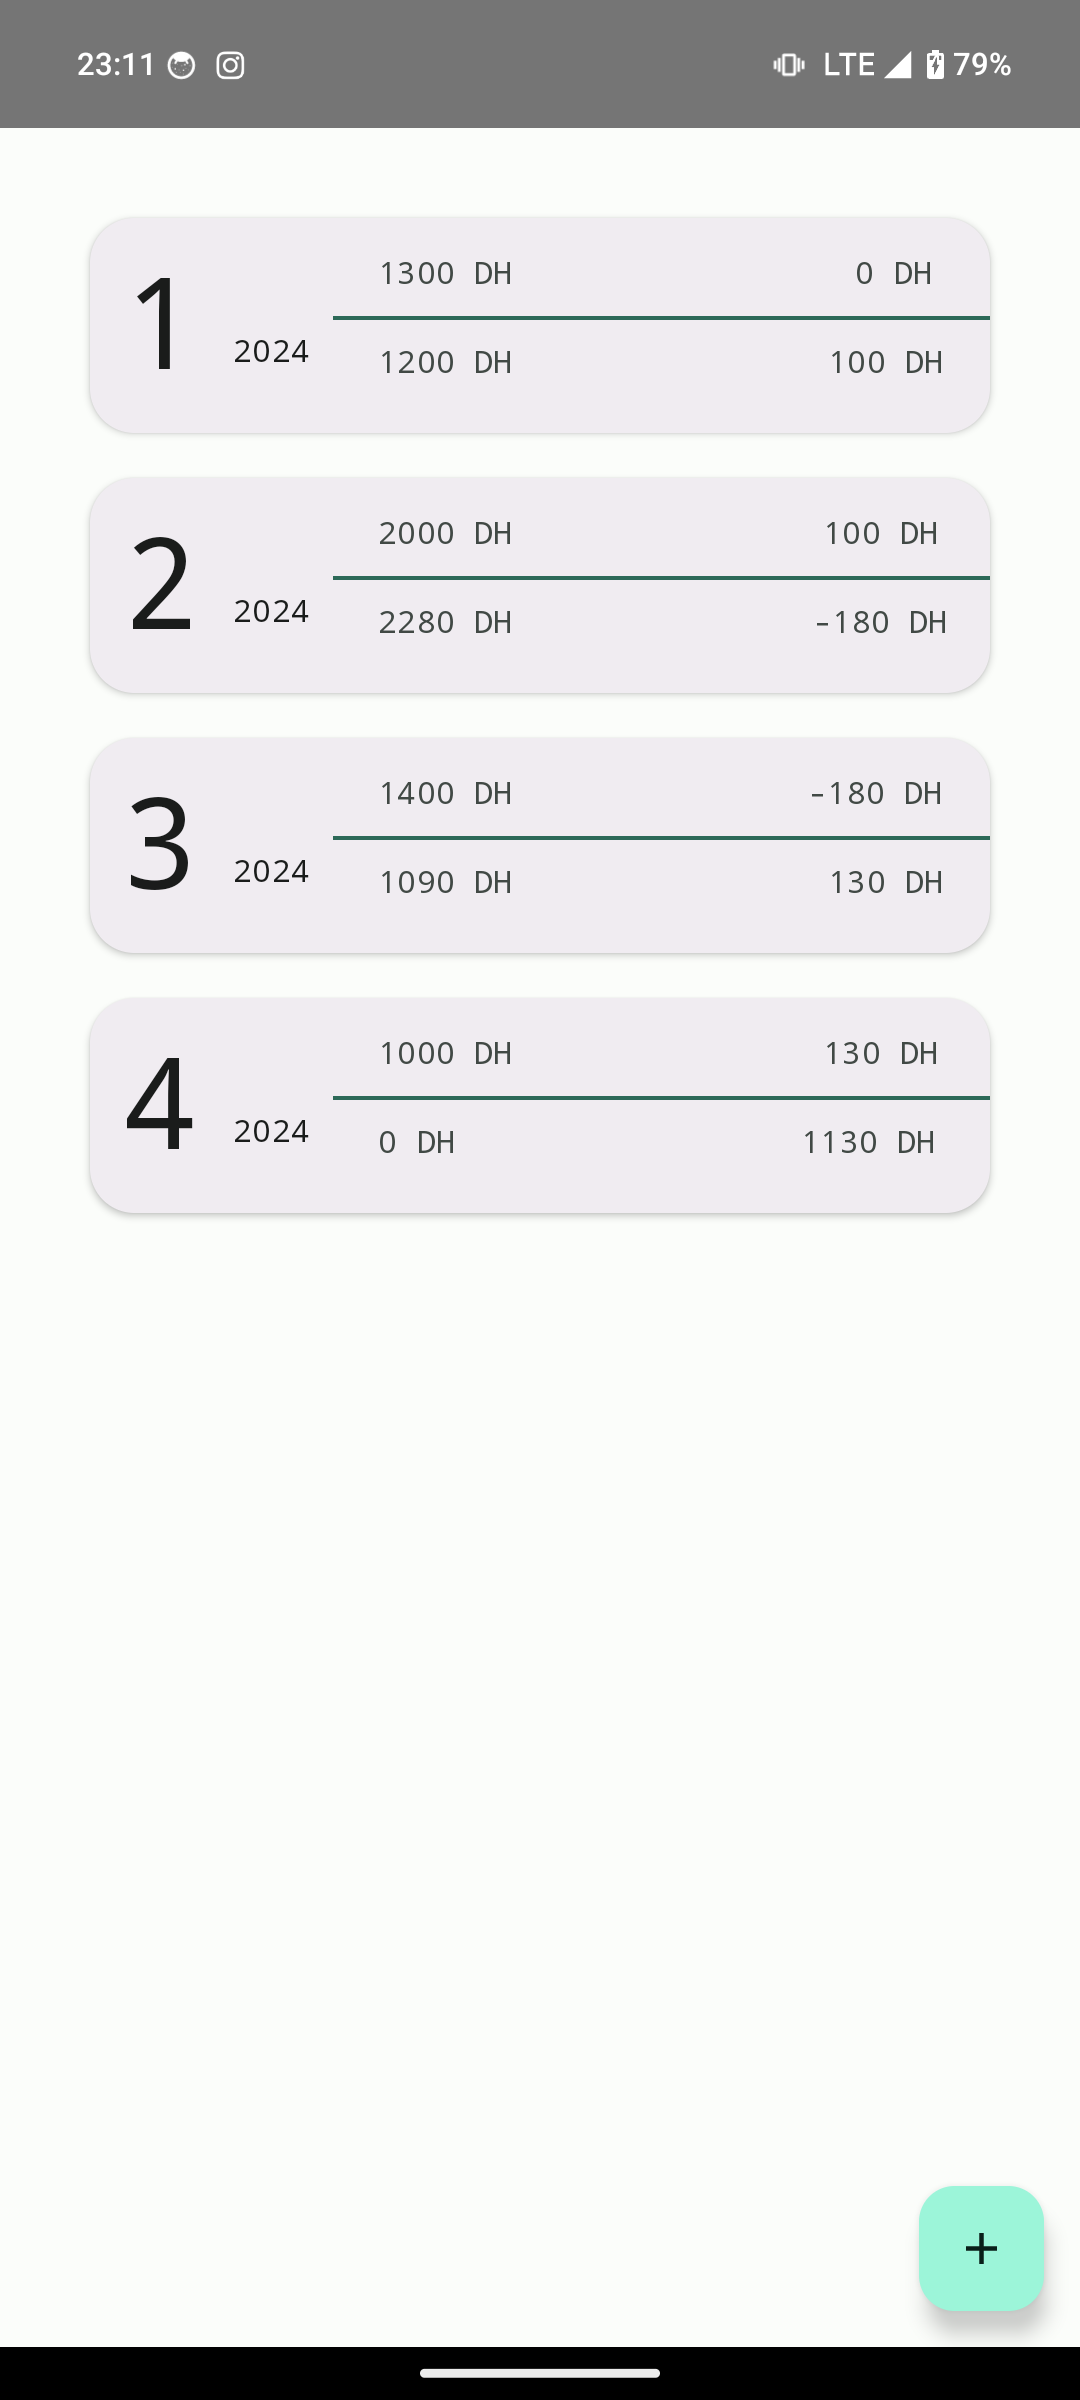
\includegraphics[width=\linewidth]{Screenshots/1.png}
          \caption{ ecran de la liste des mois}
  \end{minipage}%
  \begin{minipage}{0.20\textwidth}
    \hfill
  \end{minipage}
\begin{minipage}[t]{0.4\textwidth}
        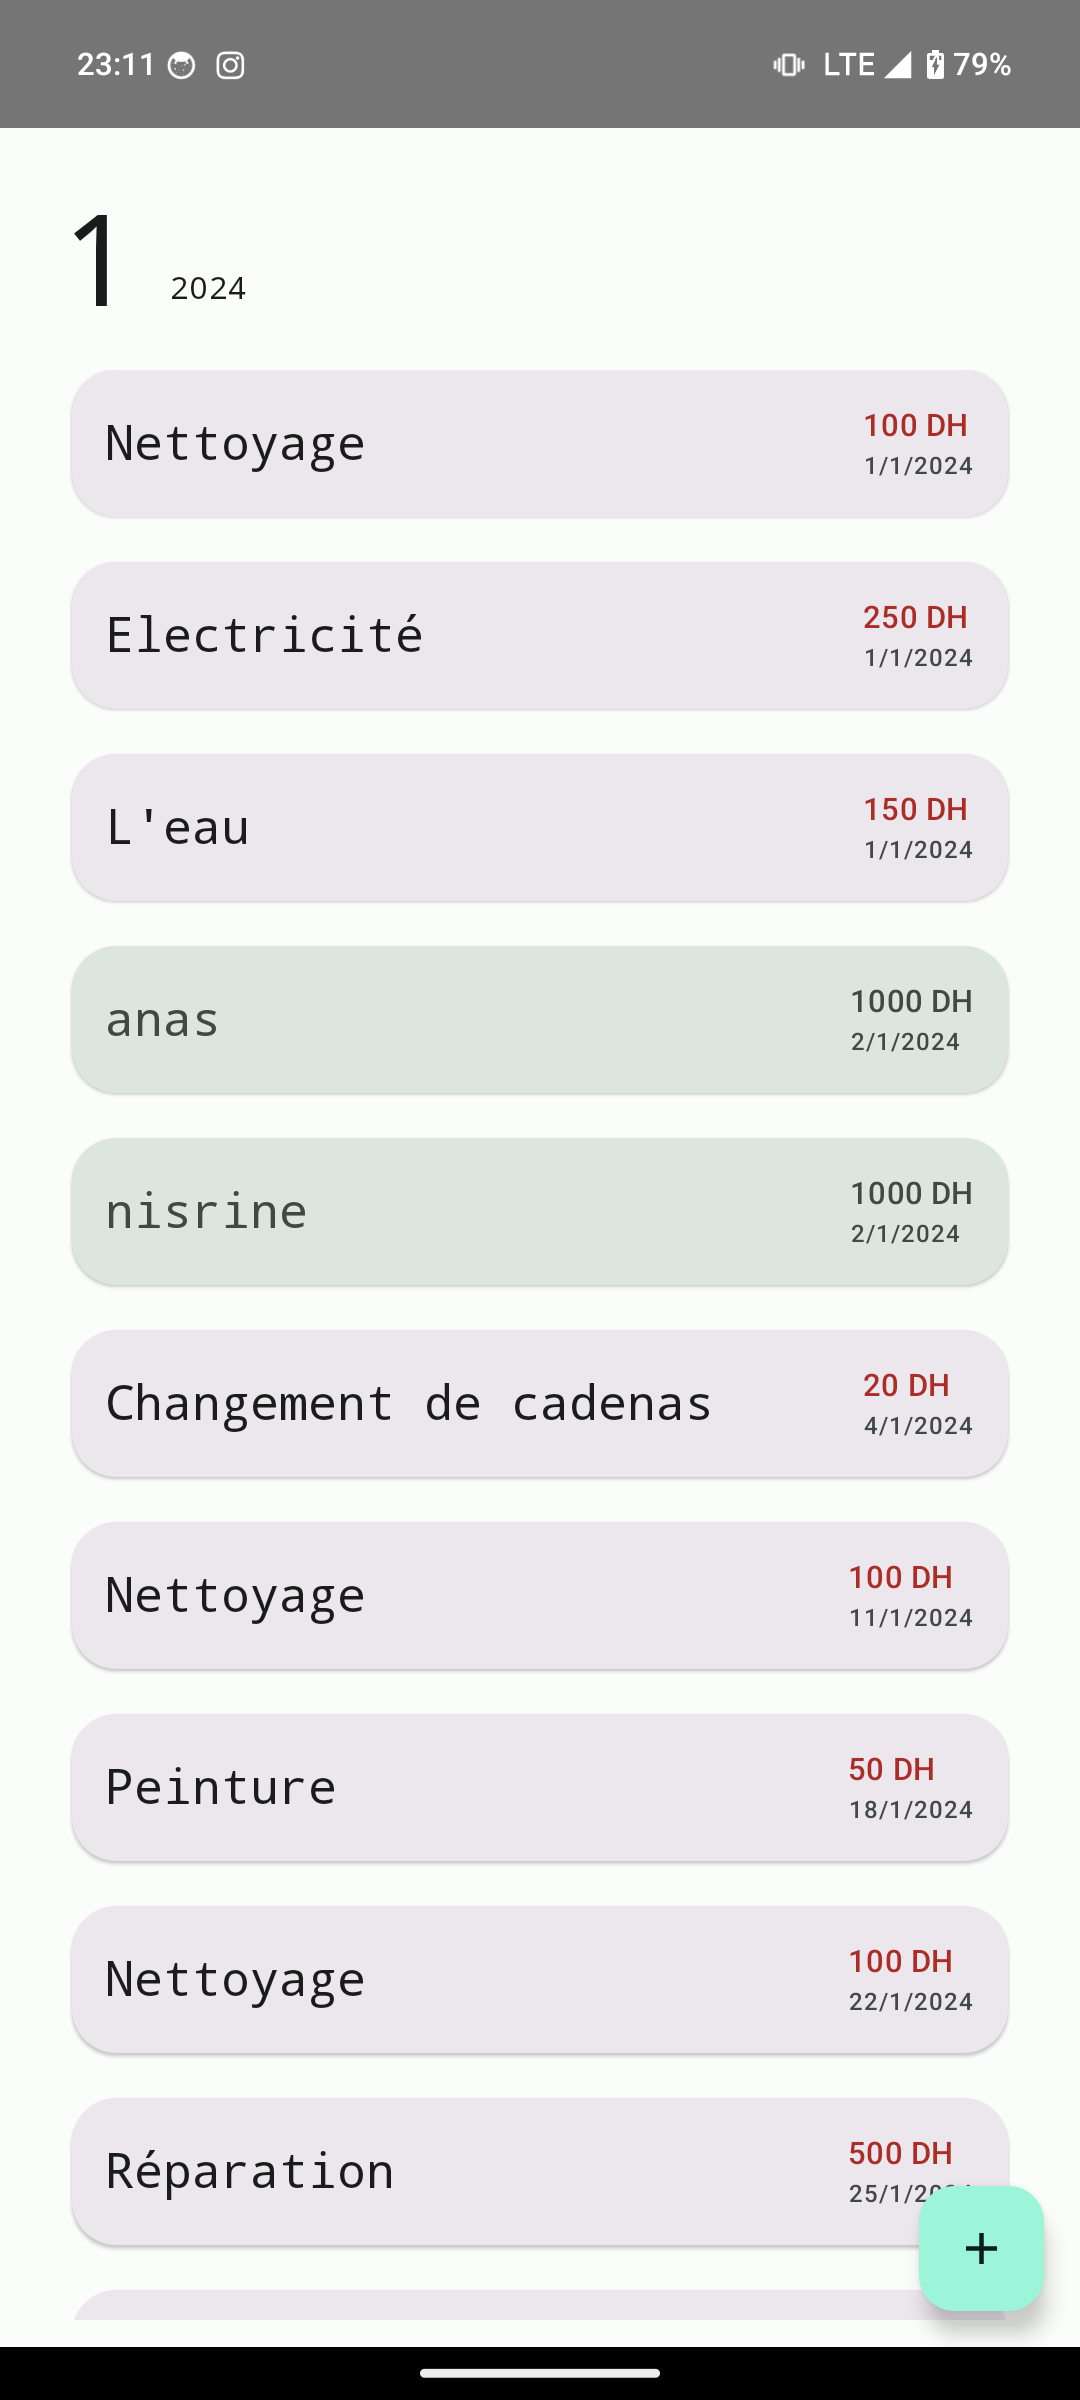
\includegraphics[width=\linewidth]{Screenshots/2.png}
        \caption{ ecran de la liste des operations de janvier 2024}
\end{minipage}%
  \end{figure}
$ $
\newpage
\section{Sprint 3}
\subsection{specification fonctionnel}
\subsubsection{gerer les cotisations}
Dans cette fonctionnalité, nous devons fournir à l'administrateur du syndicat les outils nécessaires pour ajouter ou supprimer des contributions. Chaque contribution créée doit inclure le nom de contributeur et la date à laquelle elle a eu lieu.
\subsubsection{gerer les dépenses}
Pour les dépenses, la même histoire s'applique avec une seule exception : la dépense doit inclure un type de dépense au lieu d'un nom d'utilisateur.

De plus, l'application doit permettre à l'administrateur d'ajouter de nouveaux types de dépenses ou de changer le nom des autres.

\subsection{Sprint Backlog}
\begin{center}
  \begin{tabular}{ | m{1cm} | m{9cm}| m{2cm} | m{2cm} |} 
   \hline
   GitHub ID & Sprint Backlog & Acteur & Priorité \\ [0.5ex] 
   \hline\hline
   \#18 & en tant qu'Administrateur,je veux avoir la possibilité d'ajouter un type de dépenses à la liste des dépenses prédéfinies dans l'application afin de mieux catégoriser les dépenses& Administrateur & ELEVEE \\ 
   \hline
   \#20  & En tant qu'utilisateur je veux avoir la possibilité d'ajouter une dépense à la liste des dépenses en spécifiant le type, le montant, et la date (qui doit être le jour même par défaut) afin d'enregistrer les dépenses mois. & Administrateur & ELEVEE \\
   \hline
   \#19  & En tant qu'utilisateur je veux avoir la possibilité de modifier un type de dépenses dans la liste des dépenses prédéfinies dans l'application afin de mieux catégoriser les dépenses. & Administrateur & ELEVEE \\
   \hline
   \#21  & En tant qu'utilisateur je veux avoir la possibilité d'ajouter une contribution parmi celles déjà enregistrées dans l'application afin de gérer la situation. & Administrateur & ELEVEE \\
   \hline
   \#20  & En tant qu'utilisateur je veux avoir la possibilité de supprimer une dépense de la liste des dépenses afin d'éliminer les enregistrements incorrects. & Administrateur & MOYEN \\
   \hline
  \end{tabular}
\end{center}
\subsection{conception}
Dans le troisième sprint, nous avons abordé le reste des backlogs produits principalement parce qu'ils se concentrent tous sur la gestion des opérations. 

Nous avons dû donner à l'administrateur la possibilité de créer ou de supprimer de nouvelles contributions, d'ajouter et de modifier des types de dépenses, ainsi que de créer ou de supprimer des dépenses.

\subsubsection{diagramme de cas d'utilisation}
En analysant les backlogs des sprints sélectionnés, nous constatons qu'un seul acteur est impliqué, à savoir l'administrateur. Ce dernier est responsable des actions suivantes : l'ajout ou la suppression d'une dépense, l'ajout ou la modification d'un type de dépense, ainsi que l'ajout ou la suppression d'une cotisation.
\begin{figure}[h]
    \centering
    \begin{tikzpicture}
        \begin{umlsystem}[x=3,fill=gray!10]{Sprint 3}
            \umlusecase[name=depensetype,x=0,y=2,fill=orange!30]{Gérer les types de dépenses }
            \umlusecase[name=depense,x=0,y=-0,fill=red!30]{Gérer les dépenses }
            \umlusecase[name=cotisation,y=-3,fill=green!30]{Gérer les cotisations}
            \umlusecase[name=addexpense,x=7,y=-1,fill=red!10]{Ajouter dépense}
            \umlusecase[name=updatexpense,x=7,y=-2,fill=red!10]{Supprimer dépense}

            \umlusecase[name=addexpensetype,x=7,y=1,fill=orange!10]{Ajouter type de dépense}  
            \umlusecase[name=modifyexpensetype,x=7,y=3,fill=orange!10]{Modifier type de dépense}  

            \umlusecase[name=addcontrib,x=7,y=-4,fill=green!10]{Ajouter cotisation}
            \umlusecase[name=deletecontrib,x=7,y=-5,fill=green!10]{Supprimer cotisation}
            \end{umlsystem}
            \umlactor[x=-2,y=-1]{administrateur}

        \umlassoc[anchor1=0 , anchor2=180]{administrateur}{depensetype}
        \umlassoc[anchor1=0 , anchor2=180]{administrateur}{depense}
        \umlassoc[anchor1=0 , anchor2=180]{administrateur}{cotisation}
        \umlHVextend[name=ext,anchor1=180 , anchor2=-90]{addexpensetype}{depensetype}
        \umlHVextend[name=ext,anchor1=180 , anchor2=90]{modifyexpensetype}{depensetype}
        \umlHVextend[name=ext,anchor1=180 , anchor2=-10]{addexpense}{depense}
        \umlHVextend[name=ext,anchor1=180 , anchor2=-90]{updatexpense}{depense}
        \umlHVextend[name=ext,anchor1=180 , anchor2=-10]{addcontrib}{cotisation}
        \umlHVextend[name=ext,anchor1=180 , anchor2=-30]{deletecontrib}{cotisation}

       % \umlHVinclude[name=incl]{addSpending}{auth}
        %\umlHVinclude[name=incl,anchor1=30 , anchor2=300]{addBudget}{auth}

    \end{tikzpicture}
 \caption{Le diagramme de Class pour Sprint 3}
\end{figure}

%and this is a reference to the usecase fig : \ref{fig : usecase 1}

$ $
\subsubsection{diagramme de classe}
En suivant le même principe, nous avons créé deux vues où l'administrateur peut ajouter des contributions et des dépenses. Ces deux vues utilisent des UiStates (ContributionUiState et ExpenseUiState) pour obtenir les données à afficher sur l'interface utilisateur.

Pour les modèles, nous avons utilisé les mêmes modèles créés lors du deuxième sprint.

Nous avons également chargé l'interface DataService et la classe FireBaseDataService avec les fonctions nécessaires pour atteindre les objectifs de ce sprint. Nous avons ajouté :
\begin{enumerate}
  \item addExpenseType : nous permet d'ajouter un nouveau type de dépense
  \item updateExpenseType : met à jour le nom d'un type de dépense existant
  \item addOperation : pour les contributions ou les dépenses, cette fonction nous permet d'ajouter une nouvelle opération à la base de données et de mettre à jour le mois concerné en conséquence (mise à jour du solde créditeur ou débiteur)
  \item removeOperation : également pour les contributions et les dépenses, cette fonction supprime l'enregistrement de l'opération concernée et met à jour le mois concerné en conséquence.
\end{enumerate}
    
Pour ces deux vues, nous avons utilisé OperationViewModel pour gérer la logique derrière les vues implémentées. Il contient toutes les fonctions différentes appelées par l'interface utilisateur et dispose des fonctions nécessaires pour mettre à jour les vues en fonction des réponses du service ou des interactions de l'utilisateur.

Il convient de noter que les opérations liées à la suppression des opérations (qu'il s'agisse de cotisations ou de dépenses) sont gérées via le MonthViewModel, car nous avons opté pour la gestuelle de glissement pour supprimer les opérations.

\begin{figure}
        \begin{tikzpicture}

        \umlclass[x=0,y=-3,type=interface,scale = 0.8,fill=blue!10]{DataService}{
            + users : Flow<List<User>$ $>\\
            + expensesTypes: Flow<List<SpendType>$ $>\\
            + monthList: Flow<List<Month>$ $>\\
          }{ 
            + getOperationsFlow(id: String): Flow<List<Operation>$ $> :Unit\\ 
            + addExpenseType(name: String, onResult: () -> Unit) : Unit\\
            + updateExpenseType(id: String, newname: String, onResult: () -> Unit) : Unit \\
            + addOperation (op :Operation, onResult: () -> Unit) : Unit \\
            + removeOperation(op: Operation, onResult: ()->Unit) : Unit 
          }

          \umlclass[x=0,y=3,scale=0.8,fill=blue!10]{FireBaseDataService}{
            + auth: FirebaseAuth\\
            + store : FirebaseFirestore\\
           % - OPVALUE : String \\
           % - OPTYPE : String \\
           % - OPDATE : String \\
           % - OPREF : String \\
           % - PREV\_BALANCE : String \\
           % - CURR\_BALANCE : String \\
           % - DEBIT : String \\
           % - CREDIT : String \\
           % - MONTHDATE : String \\
           % - LIST : String \\
           % - USERS : String \\
           % - USERS : String \\
            - MONTH\_DATA\_COLLECTION : String\\
            - SPEND\_TYPES\_COLLECTION : String\\
            - LIST : String\\
          }{
            + Constructor(auth: FirebaseAuth,store : FirebaseFirestore)\\
            - getexpenseType(id:String) : SpendType\\
            - getUser(id:String) : User\\
            - onFirestoreException(e: java.lang.Exception) : Unit\\
            - addExpenseType(name: String, onResult: () -> Unit) : Unit\\
            - updateExpenseType(id: String, newname: String, onResult: () -> Unit) : Unit\\
            - updateMonth(m: Month, onResult: () -> Unit) : Unit\\
            - addMonth(m: Month) : Month\\
            - getMonthDateBasedOnOpDate(date:Date) : Date\\
            - getMonthByDateOrCreateNewOne(time: Date): Month  
          } 
          \umlclass[x=8,y=3,scale = 0.6,fill=white!10]{Month}{
            + id :String \\
            + prevBalance : Long \\
            + currBalance: Long \\
            + monthDate : Date \\
            + debit : Long \\
            + credit : Long
          }{
          }

          \umlclass[x=9,y=0,scale = 0.6,fill=white!10]{SpendType}{
            + id : String\\
            + name : String
          }{
          } 
          \umlclass[x=8,y=-3,scale = 0.6,fill=white!10]{User}{
            - IS\_ADMIN:Boolean \\
            name : String \\
            familyname : String \\
            id : String \\
            email : String
          }{
          } 

          \umlclass[x=1,y=-7,scale = 0.6,fill=orange!10]{ContributionUiState}{
            + user : User \\
            + date : Date \\
            + amount : Int \\
            + pendingOperation : Boolean \\
          }{}

          \umlclass[x=5,y=-7,scale = 0.6,fill=orange!10]{ExpenseuiState}{
            + type : String \\
            + date : Date \\
            + amount : Int \\
            + visibleName : String \\
            + ref : String \\
            + pendingOperation : Boolean \\
          }{}

          \umlclass[x=9,y=-12,scale = 0.6,fill=white!10]{Operation}{
            + id :String \\
            - ref:String \\
            + type :String \\
            + value : Long \\
            + date : Date  \\
            + Spendtype : SpendType \\
            + user : User \\
          }{
          } 
          \umlclass[x=-3,y=-7,scale = 0.6,fill=yellow!10]{ViewModel}{
            }{
            } 
          
          \umlclass[x=-1,y=-12,scale = 0.6,fill=yellow!10]{OperationViewModel}{
              - dataService: DataService\\
              - CONTRIBUTION : String \\
              - EXPENSE : String \\
              - users : Flow<List<User>$ $> \\
              - contribiutionUiState :  MutableState<ContributionUiState> \\
              - expenseUiState : MutableState<ExpenseuiState> \\
              - expensesTypes : Flow<List<SpendType>$ $> \\
              + monthList :  Flow<List<Month>$ $> \\
            }{
              + constructor(dataService: DataService) \\ % TODO: find the correct way to represent the constructor
              + addExpense() : Unit \\
              + addexpenseResult() : Unit \\
              + addcontributionResult() : Unit\\
              + addExpenseType(id: String) : Unit \\
              + modifyExpenseType(id: String, name: String) : Unit\\
              + setNewVal(newVal: String) : Unit\\
              + onContribValueChange(newval: String) : Unit \\
              + addContribution() : Unit \\
            } 
        
        \umlinherit[geometry=|-|,anchors=50 and -50]{OperationViewModel}{ViewModel}
        \umlinherit[geometry=|-|]{FireBaseDataService}{DataService}
        
        \umlaggreg[geometry=|-,anchors=80 and 0]{Operation}{User}
        \umlaggreg[geometry=|-,anchors=50 and 0]{Operation}{SpendType}
        \umlaggreg[geometry=-|,anchors=30 and -60]{OperationViewModel}{SpendType}
        \umlaggreg[draw=black!30]{OperationViewModel}{Month}
        \umlaggreg[geometry=-|,anchors=180 and -170]{OperationViewModel}{DataService}
        \umlassoc[geometry=-|,anchors=20 and 100]{FireBaseDataService}{Month}
        \umlaggreg[geometry=-|,anchors=-20 and 120]{DataService}{Operation}
        \umlaggreg{OperationViewModel}{ContributionUiState}
        \umlaggreg{OperationViewModel}{ExpenseuiState}
        \umlassoc[geometry=-|,anchors=-20 and 130]{FireBaseDataService}{User}
        %\umlaggreg[geometry=|-,anchors=20 and 0]{MonthViewModel}{Month}
        \end{tikzpicture}
        \caption{le diagramme de Class pour Sprint 2}
        \label{fig : Class diagram Sprint 1}
    \end{figure}
$ $
\subsection{Realisation}
\subsubsection{l'acces au menu latéral}
\begin{figure}[!htbp]
  \begin{minipage}[t]{0.4\textwidth}    %% b or t, default is c
          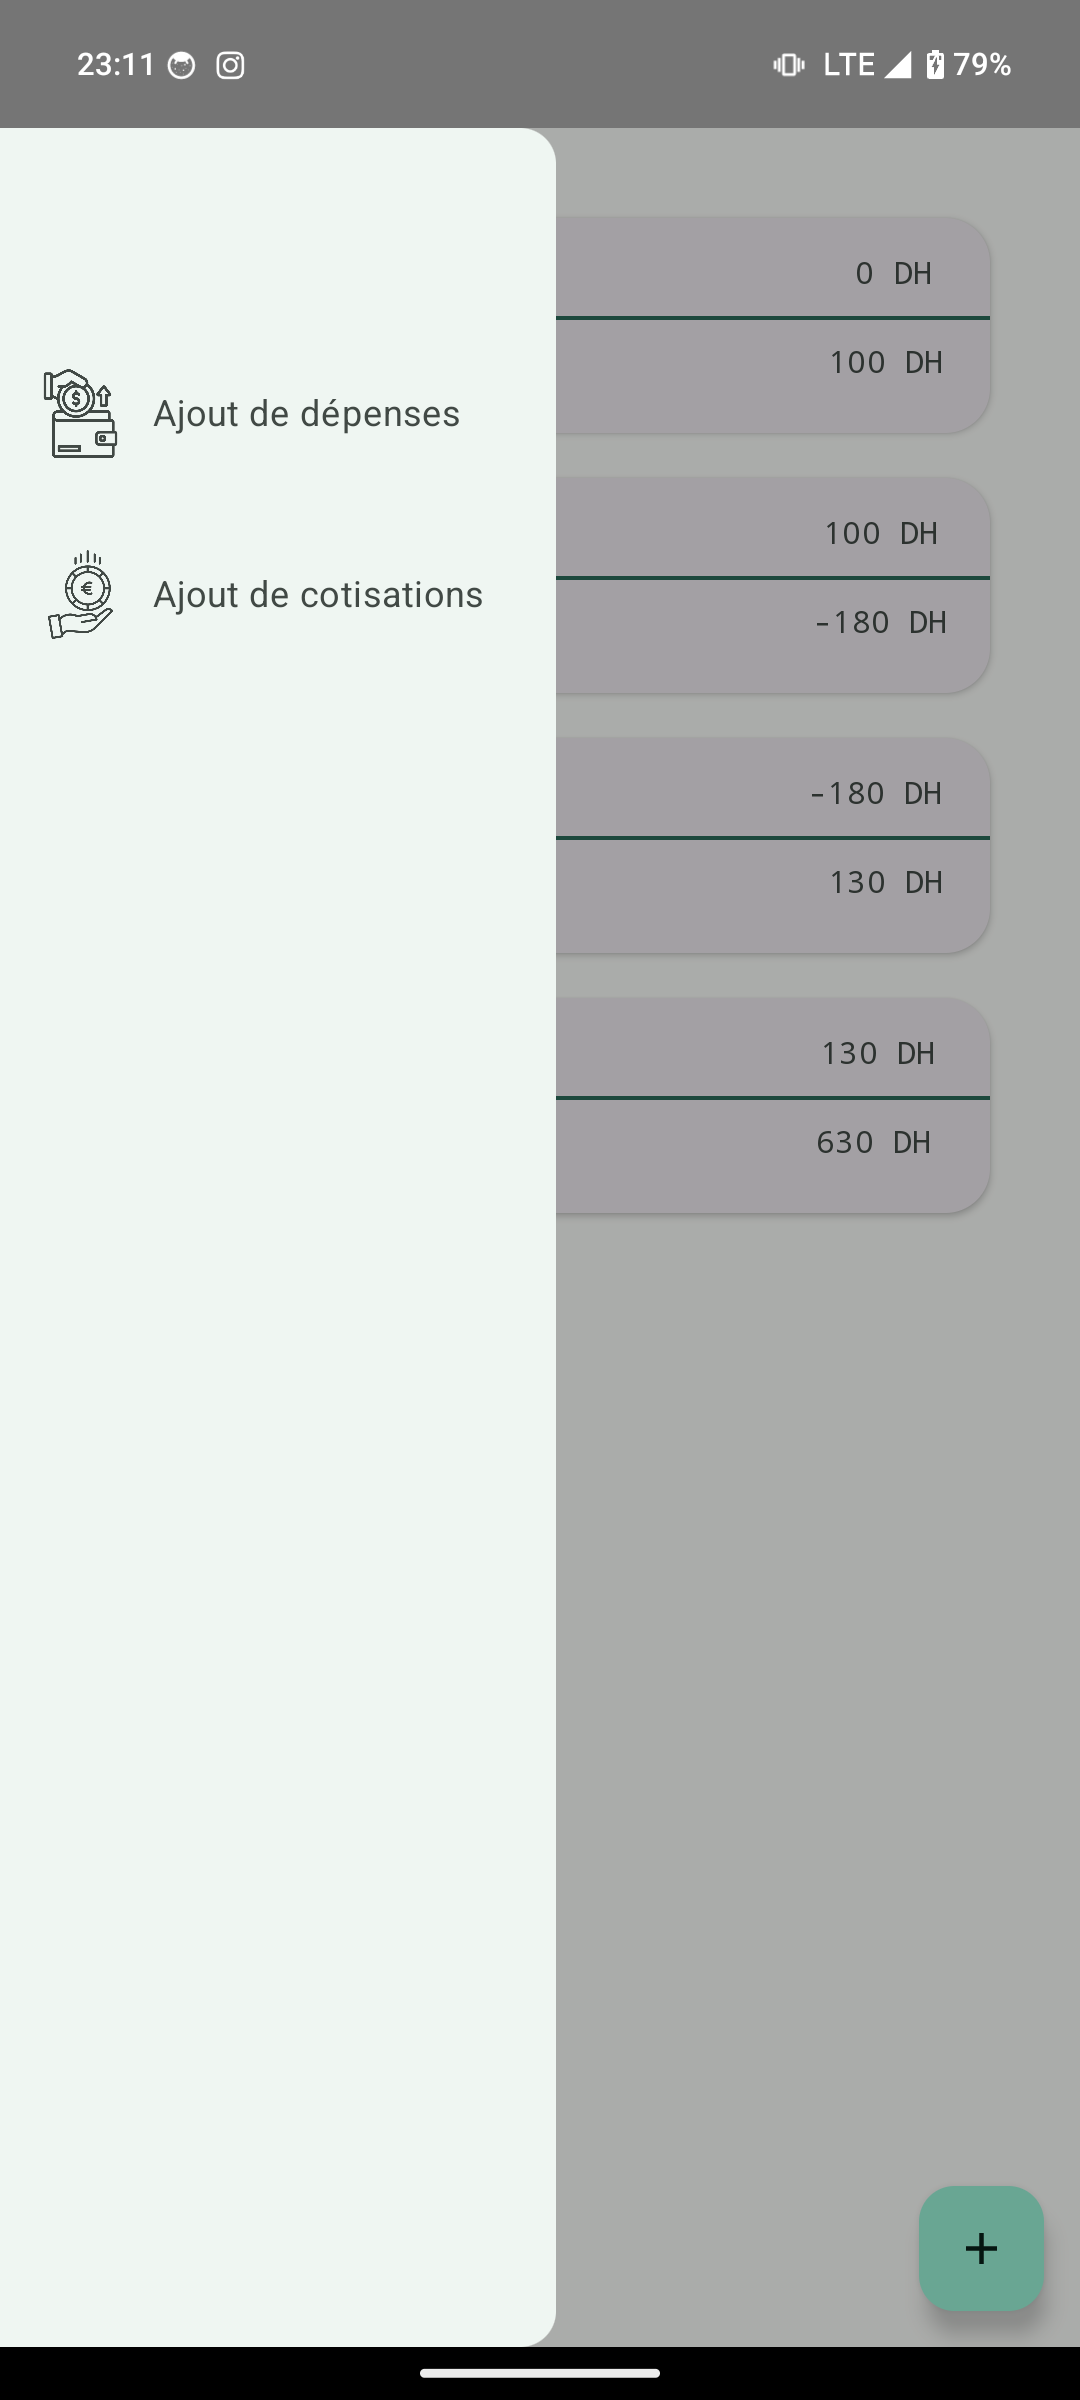
\includegraphics[width=\linewidth]{Screenshots/6.png}
          \caption{ menu latéral accesible par l'administrateur}
  \end{minipage}%
  \begin{minipage}{0.20\textwidth}
    \hfill
  \end{minipage}
\begin{minipage}[t]{0.4\textwidth}
        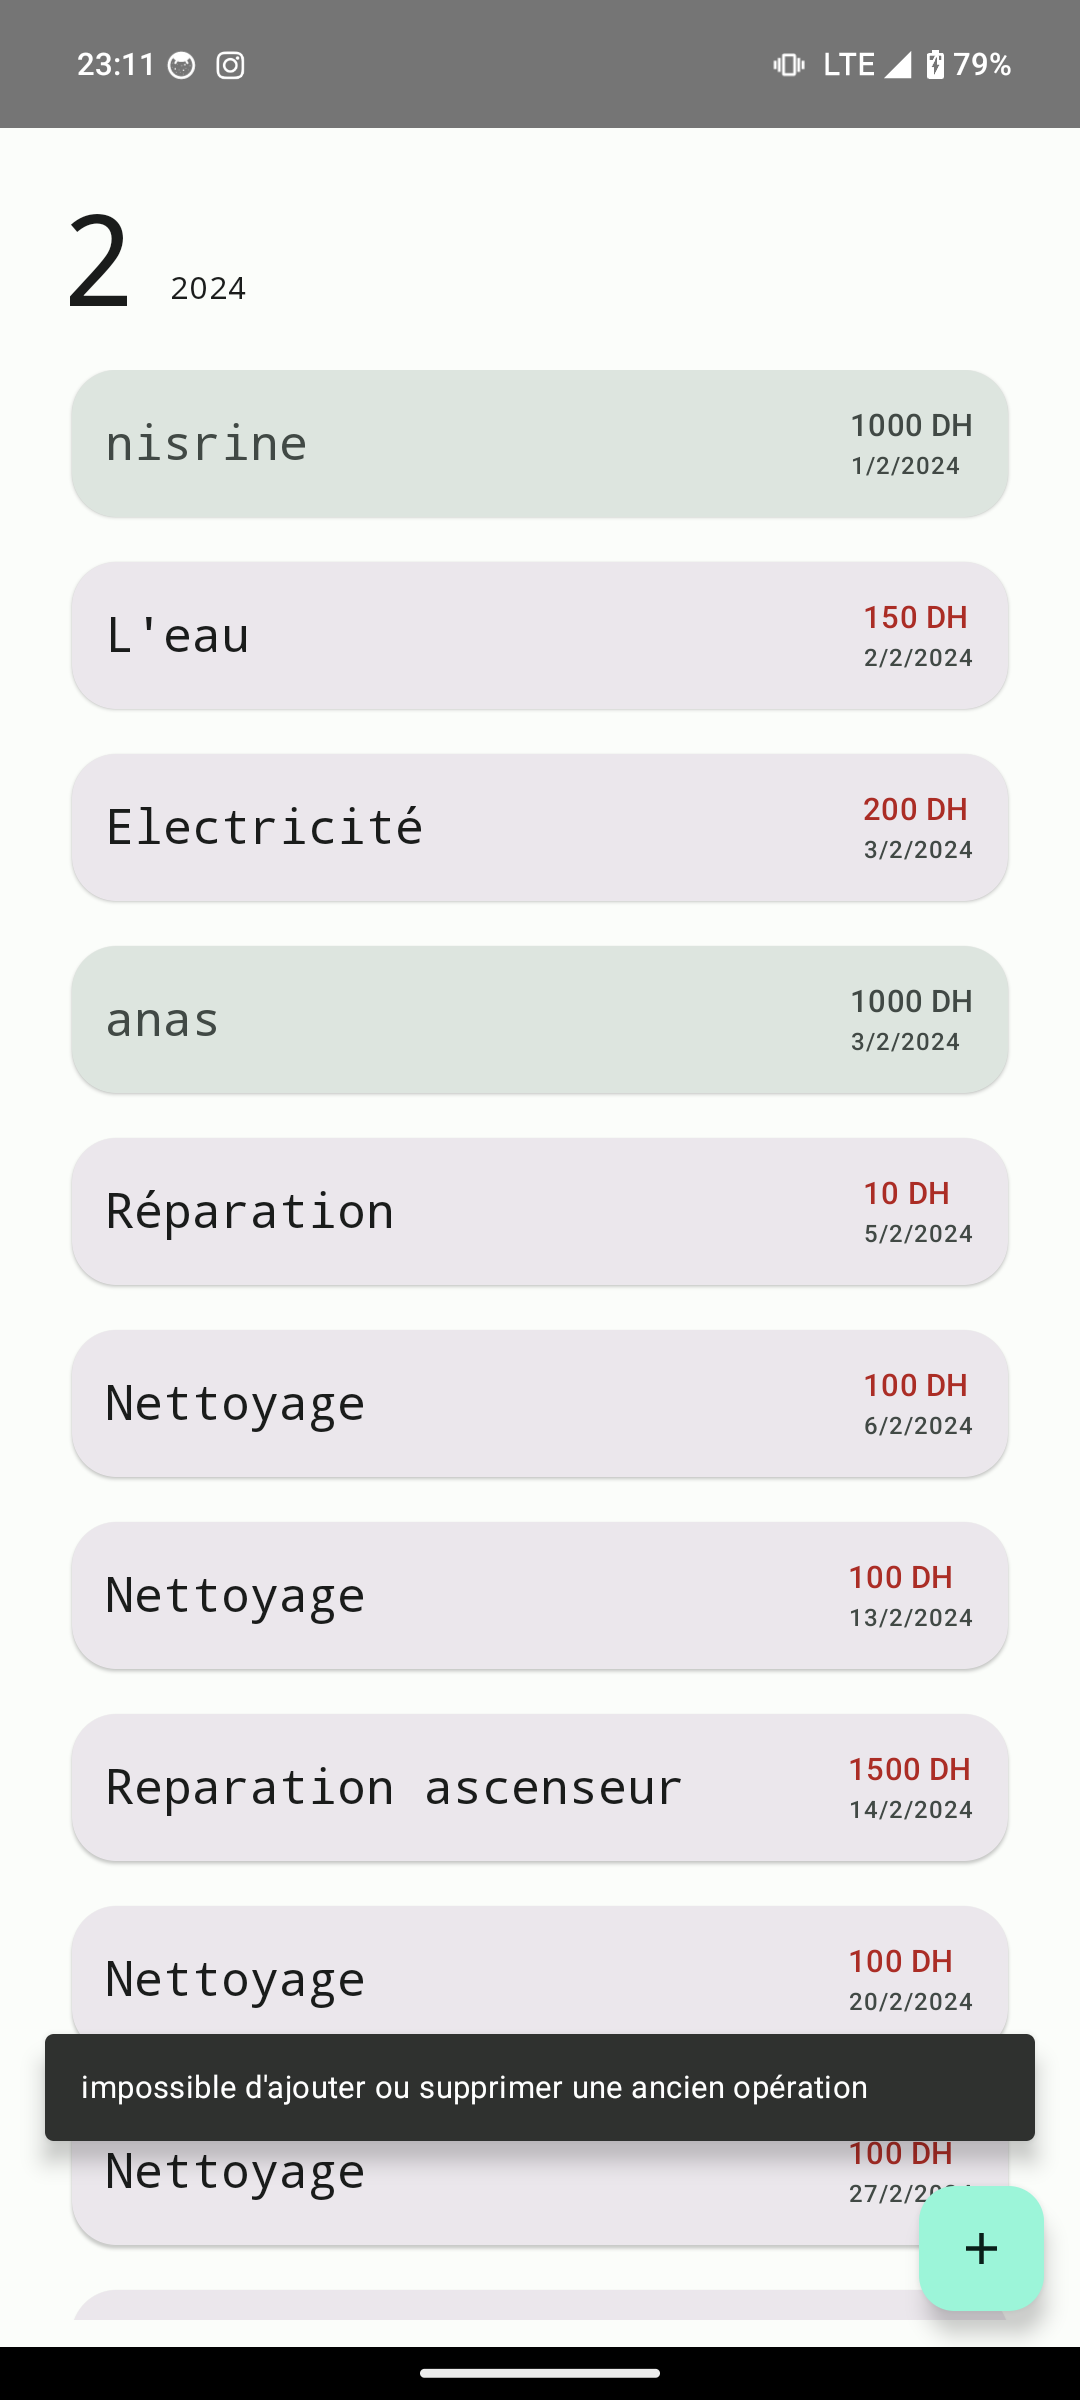
\includegraphics[width=\linewidth]{Screenshots/4.png}
        \caption{ message d'erreur si l'administrateur essaye d'ajouter ou supprimer une operation avec un date ancien}
\end{minipage}%
  \end{figure}
  \subsubsection{ajout de depense}
  \begin{figure}[!htbp]
    \begin{minipage}[t]{0.4\textwidth}    %% b or t, default is c
            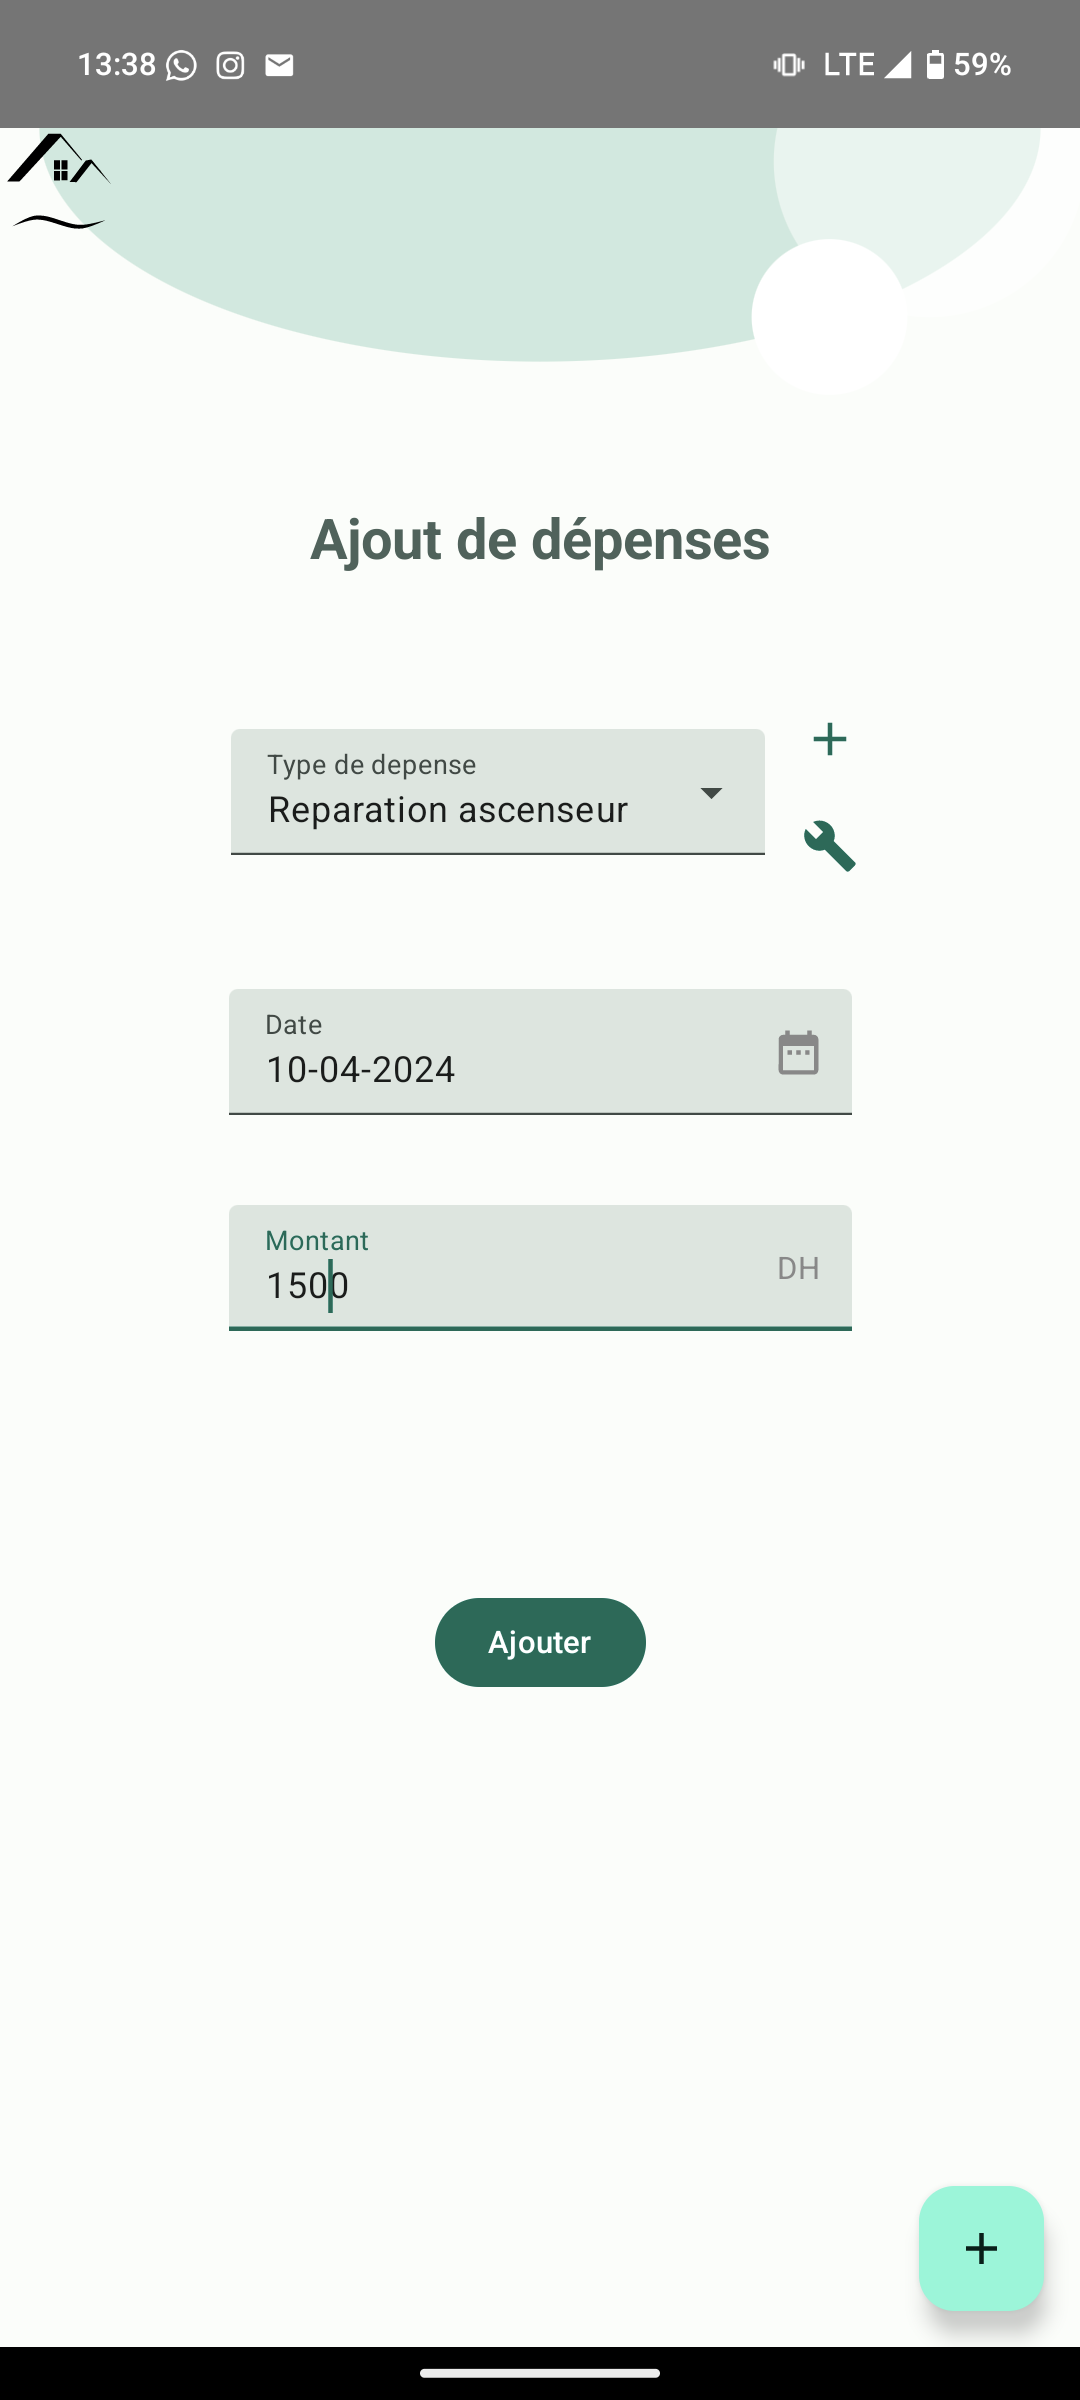
\includegraphics[width=\linewidth]{Screenshots/c2.png}
            \caption{ exemple d'interface pour ajouter des depenses}
    \end{minipage}%
    \begin{minipage}{0.20\textwidth}
      \hfill
    \end{minipage}
  \begin{minipage}[t]{0.4\textwidth}
          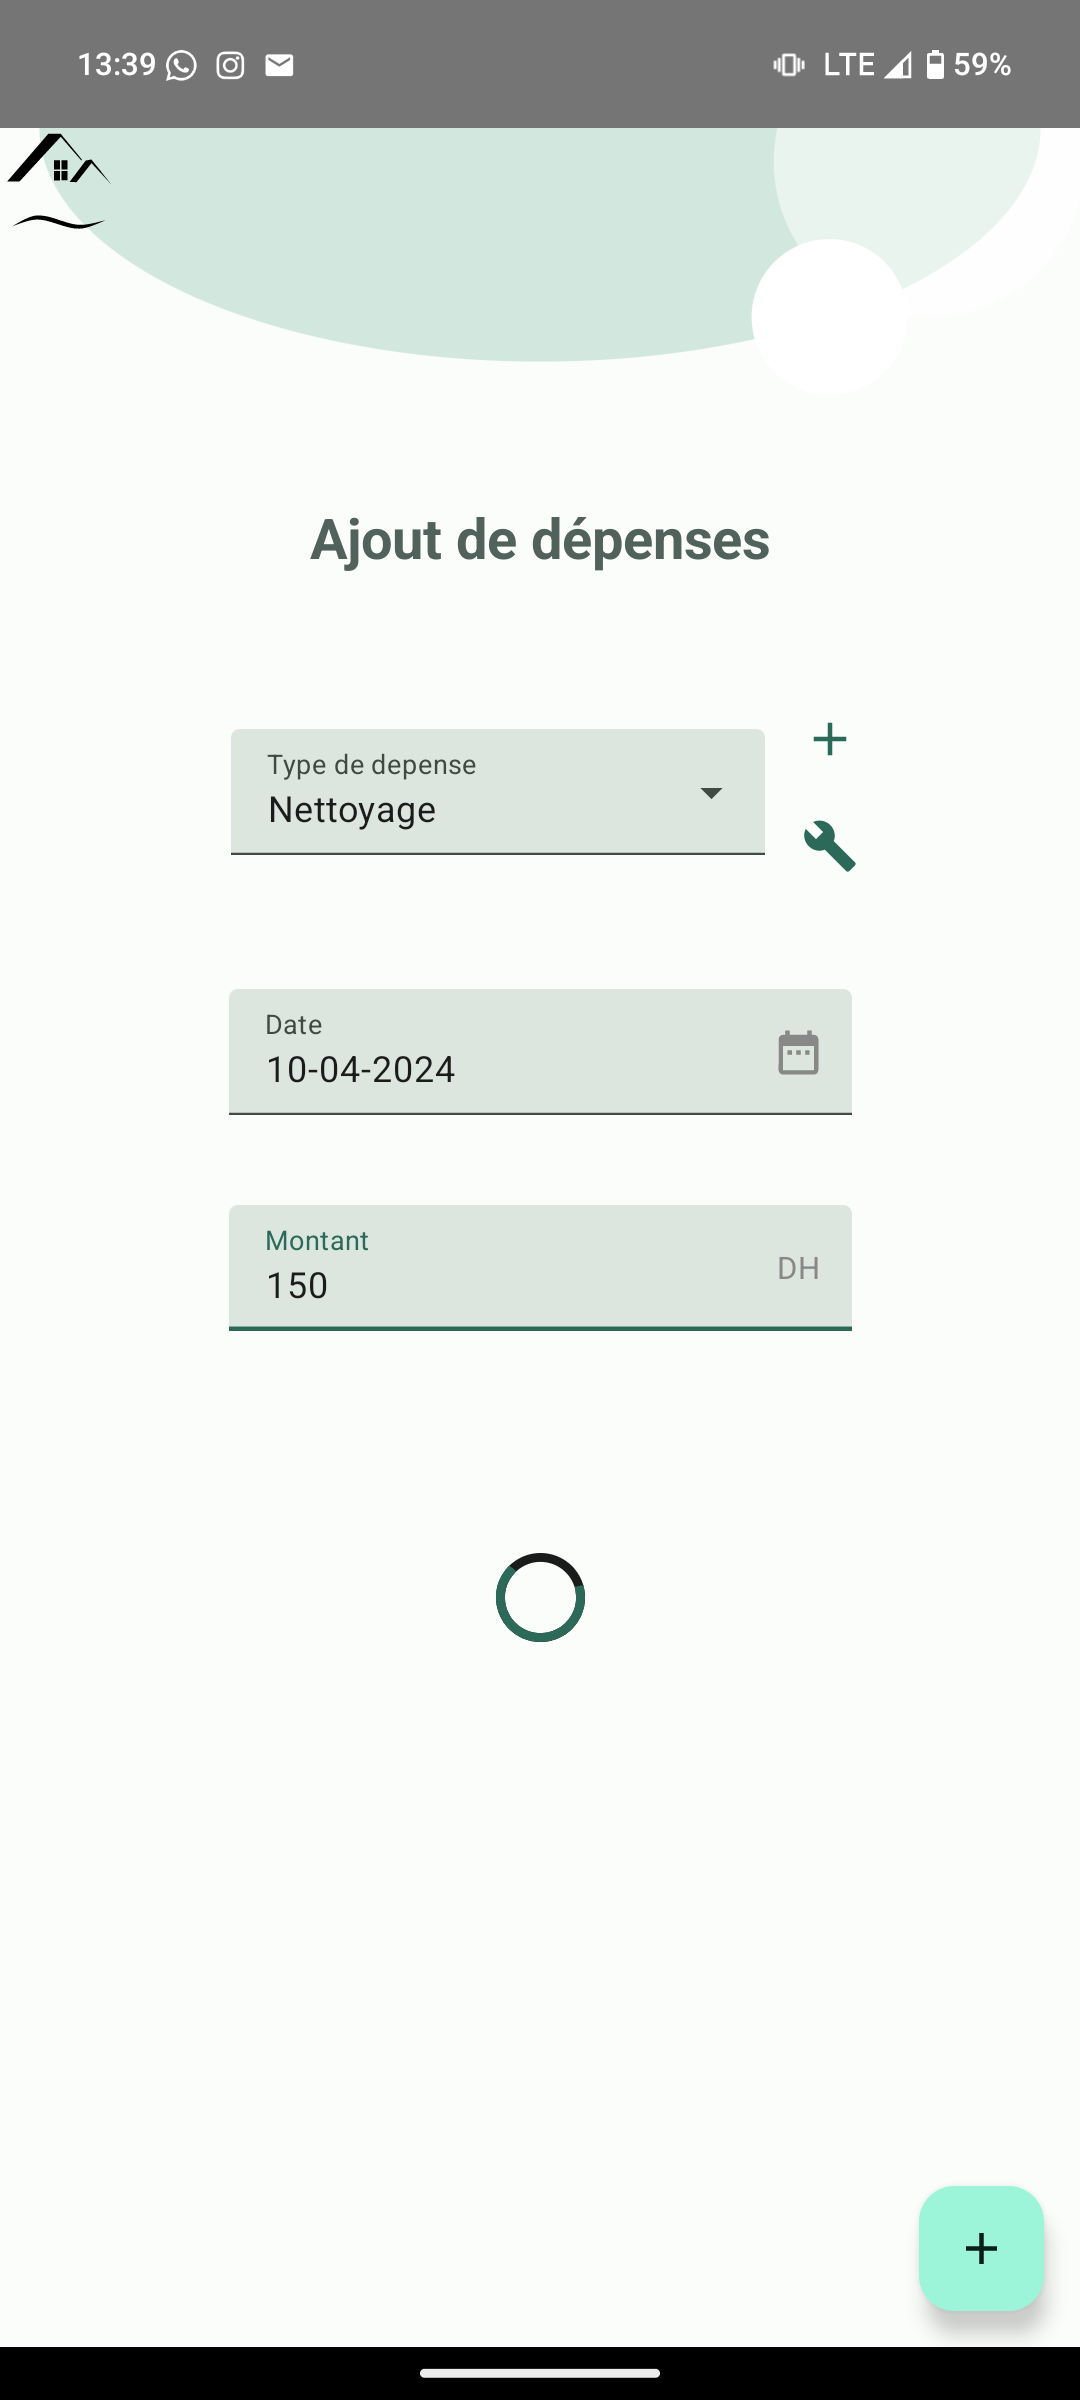
\includegraphics[width=\linewidth]{Screenshots/c5.png}
          \caption{ exemple d'opération en cours ( ajout de depense) }
  \end{minipage}%
    \end{figure}
    \begin{figure}[!htbp]
      \begin{minipage}[t]{0.4\textwidth}    %% b or t, default is c
        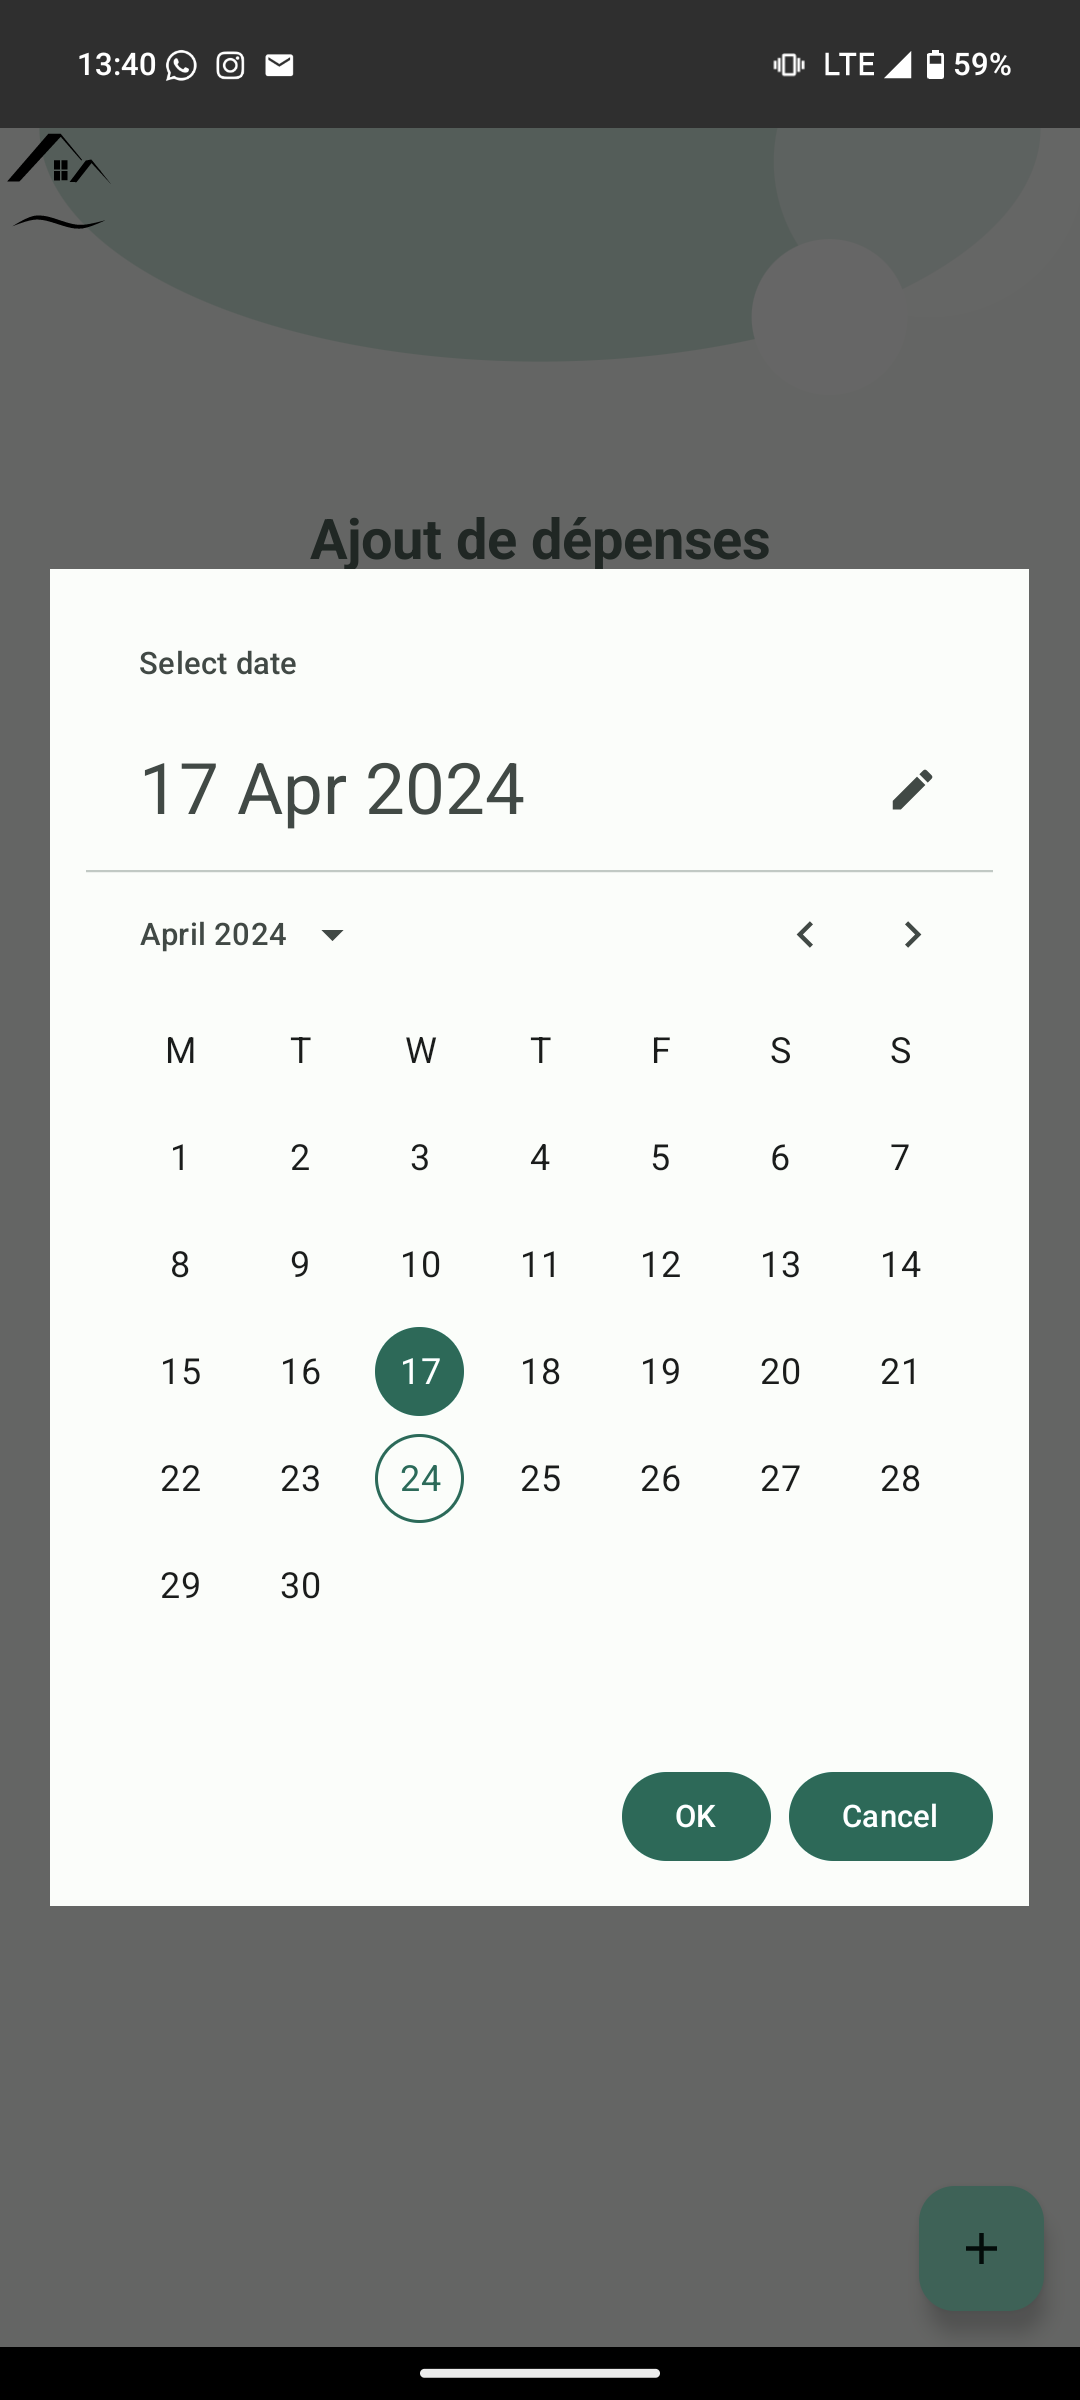
\includegraphics[width=\linewidth]{Screenshots/c7.png}
        \caption{ calendrier pour selectionner la date de depense}
          \end{minipage}%
          \begin{minipage}{0.20\textwidth}
            \hfill
          \end{minipage}
      \begin{minipage}[t]{0.4\textwidth}    %% b or t, default is c
              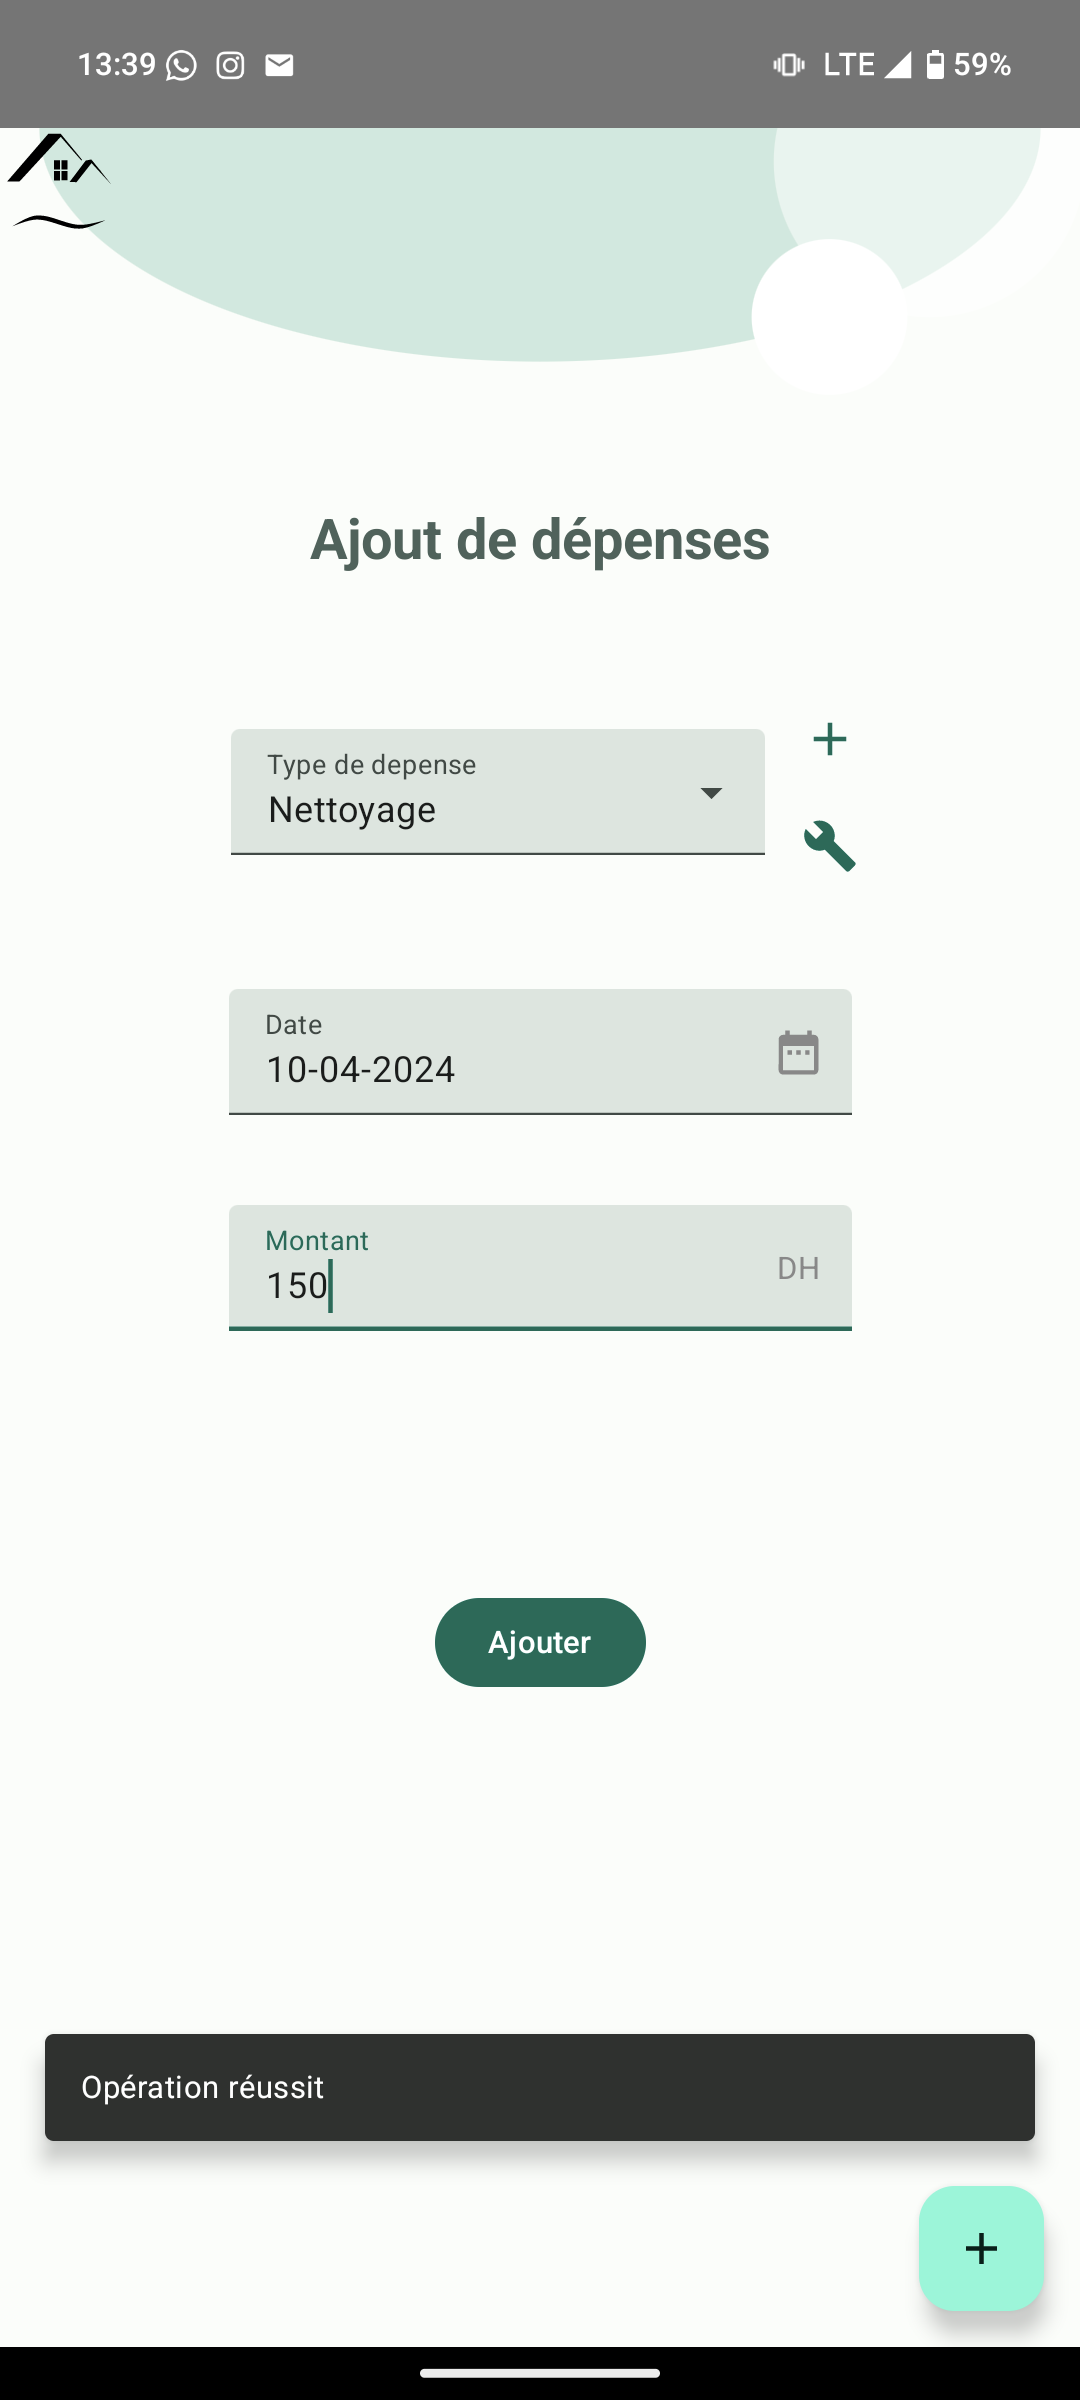
\includegraphics[width=\linewidth]{Screenshots/c6.png}
              \caption{ exemple de message de reussit d'ajout de depenses}
      \end{minipage}%
      \end{figure}

      \subsubsection{ajout et modidication de type de depense}

      \begin{figure}[!htbp]
        \begin{minipage}[t]{0.4\textwidth}    %% b or t, default is c
                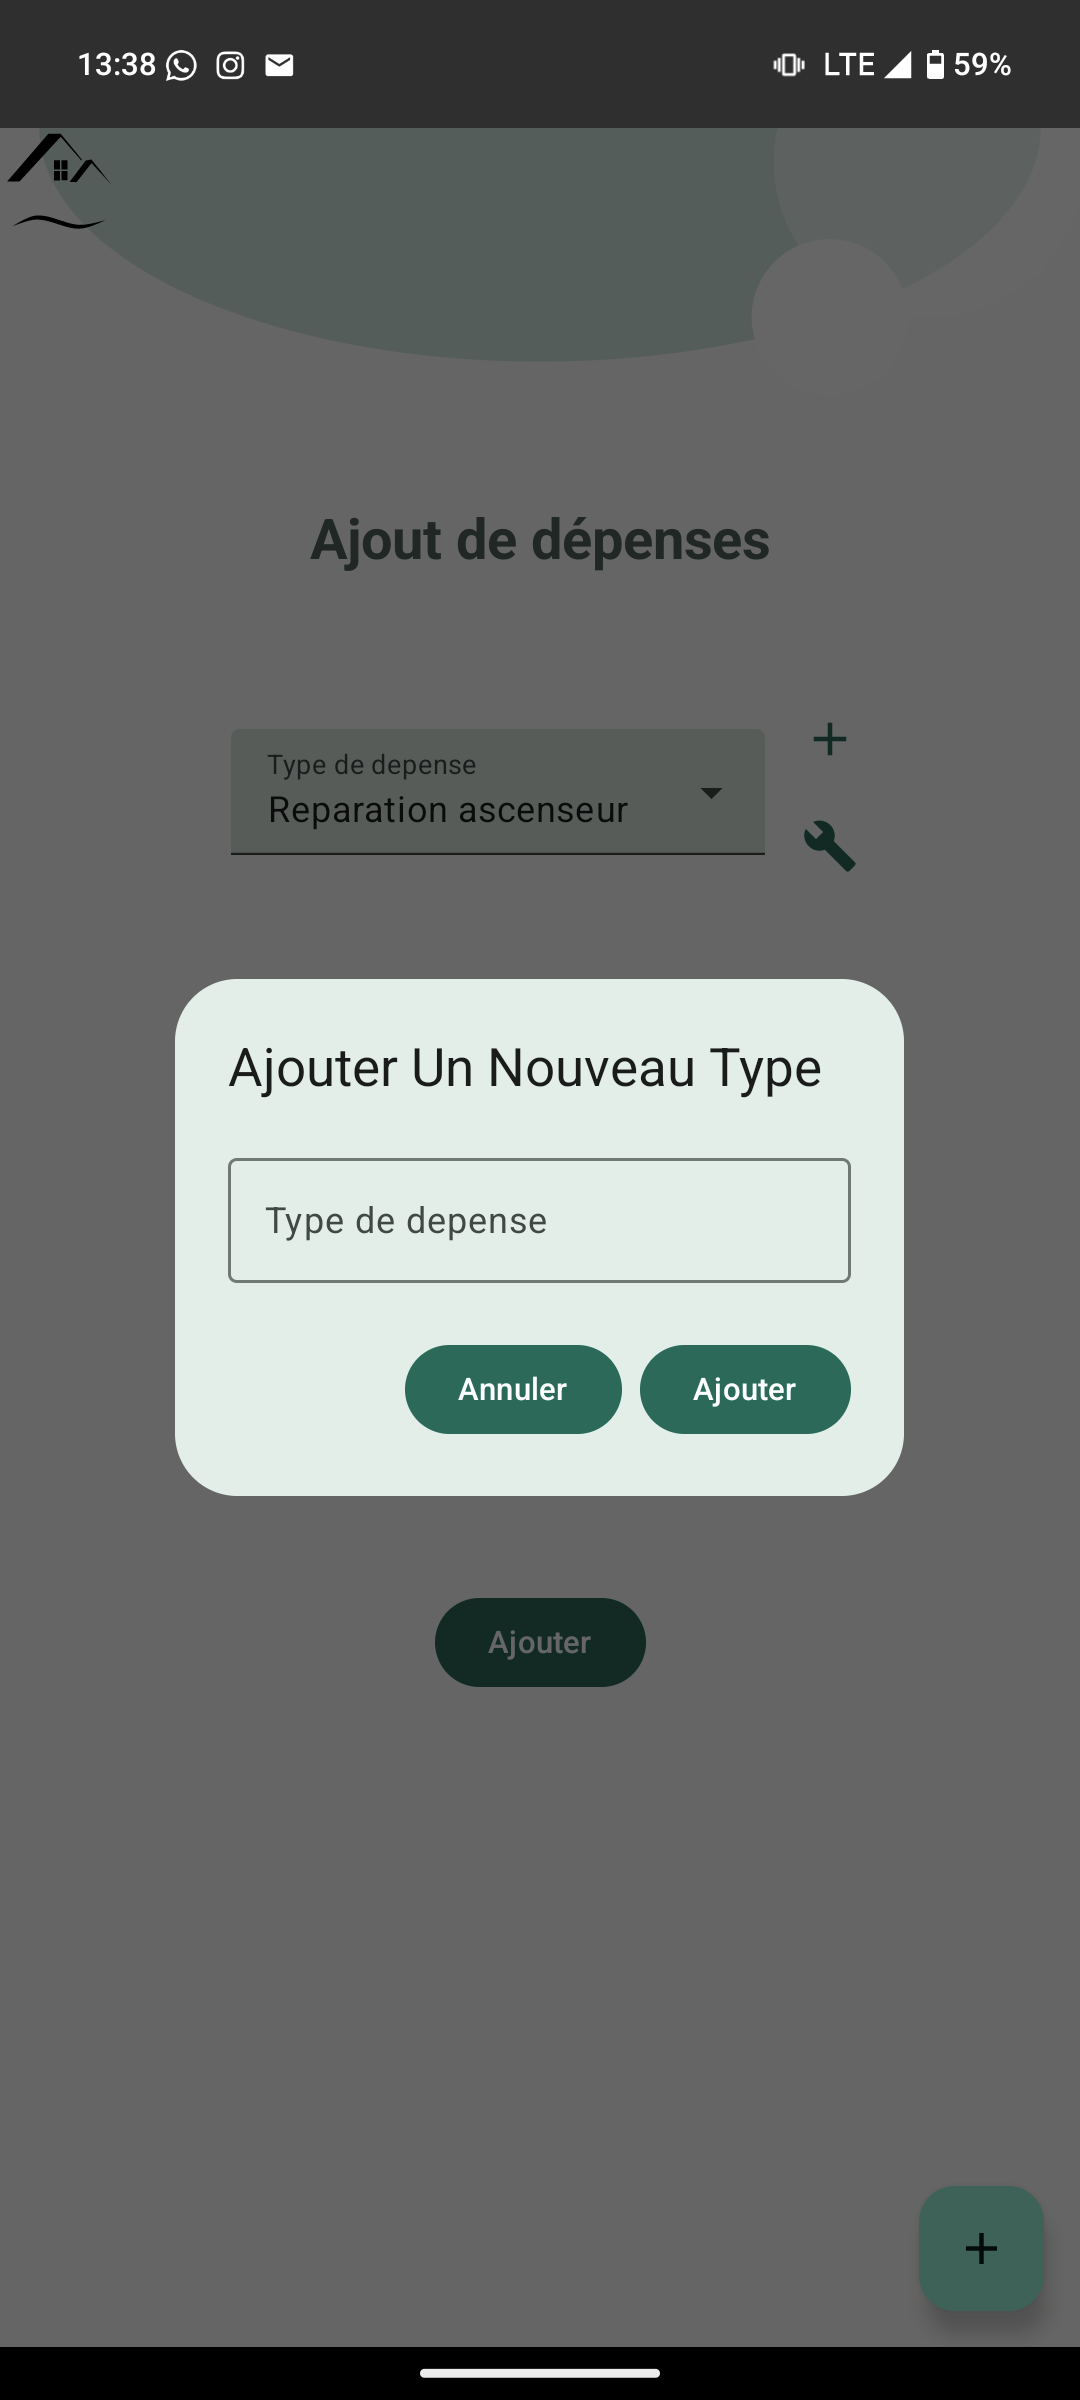
\includegraphics[width=\linewidth]{Screenshots/c3.png}
                \caption{ interface d'ajout d'un noveau type de depense a la liste des types des depenses}
        \end{minipage}%
        \begin{minipage}{0.20\textwidth}
          \hfill
        \end{minipage}
      \begin{minipage}[t]{0.4\textwidth}
              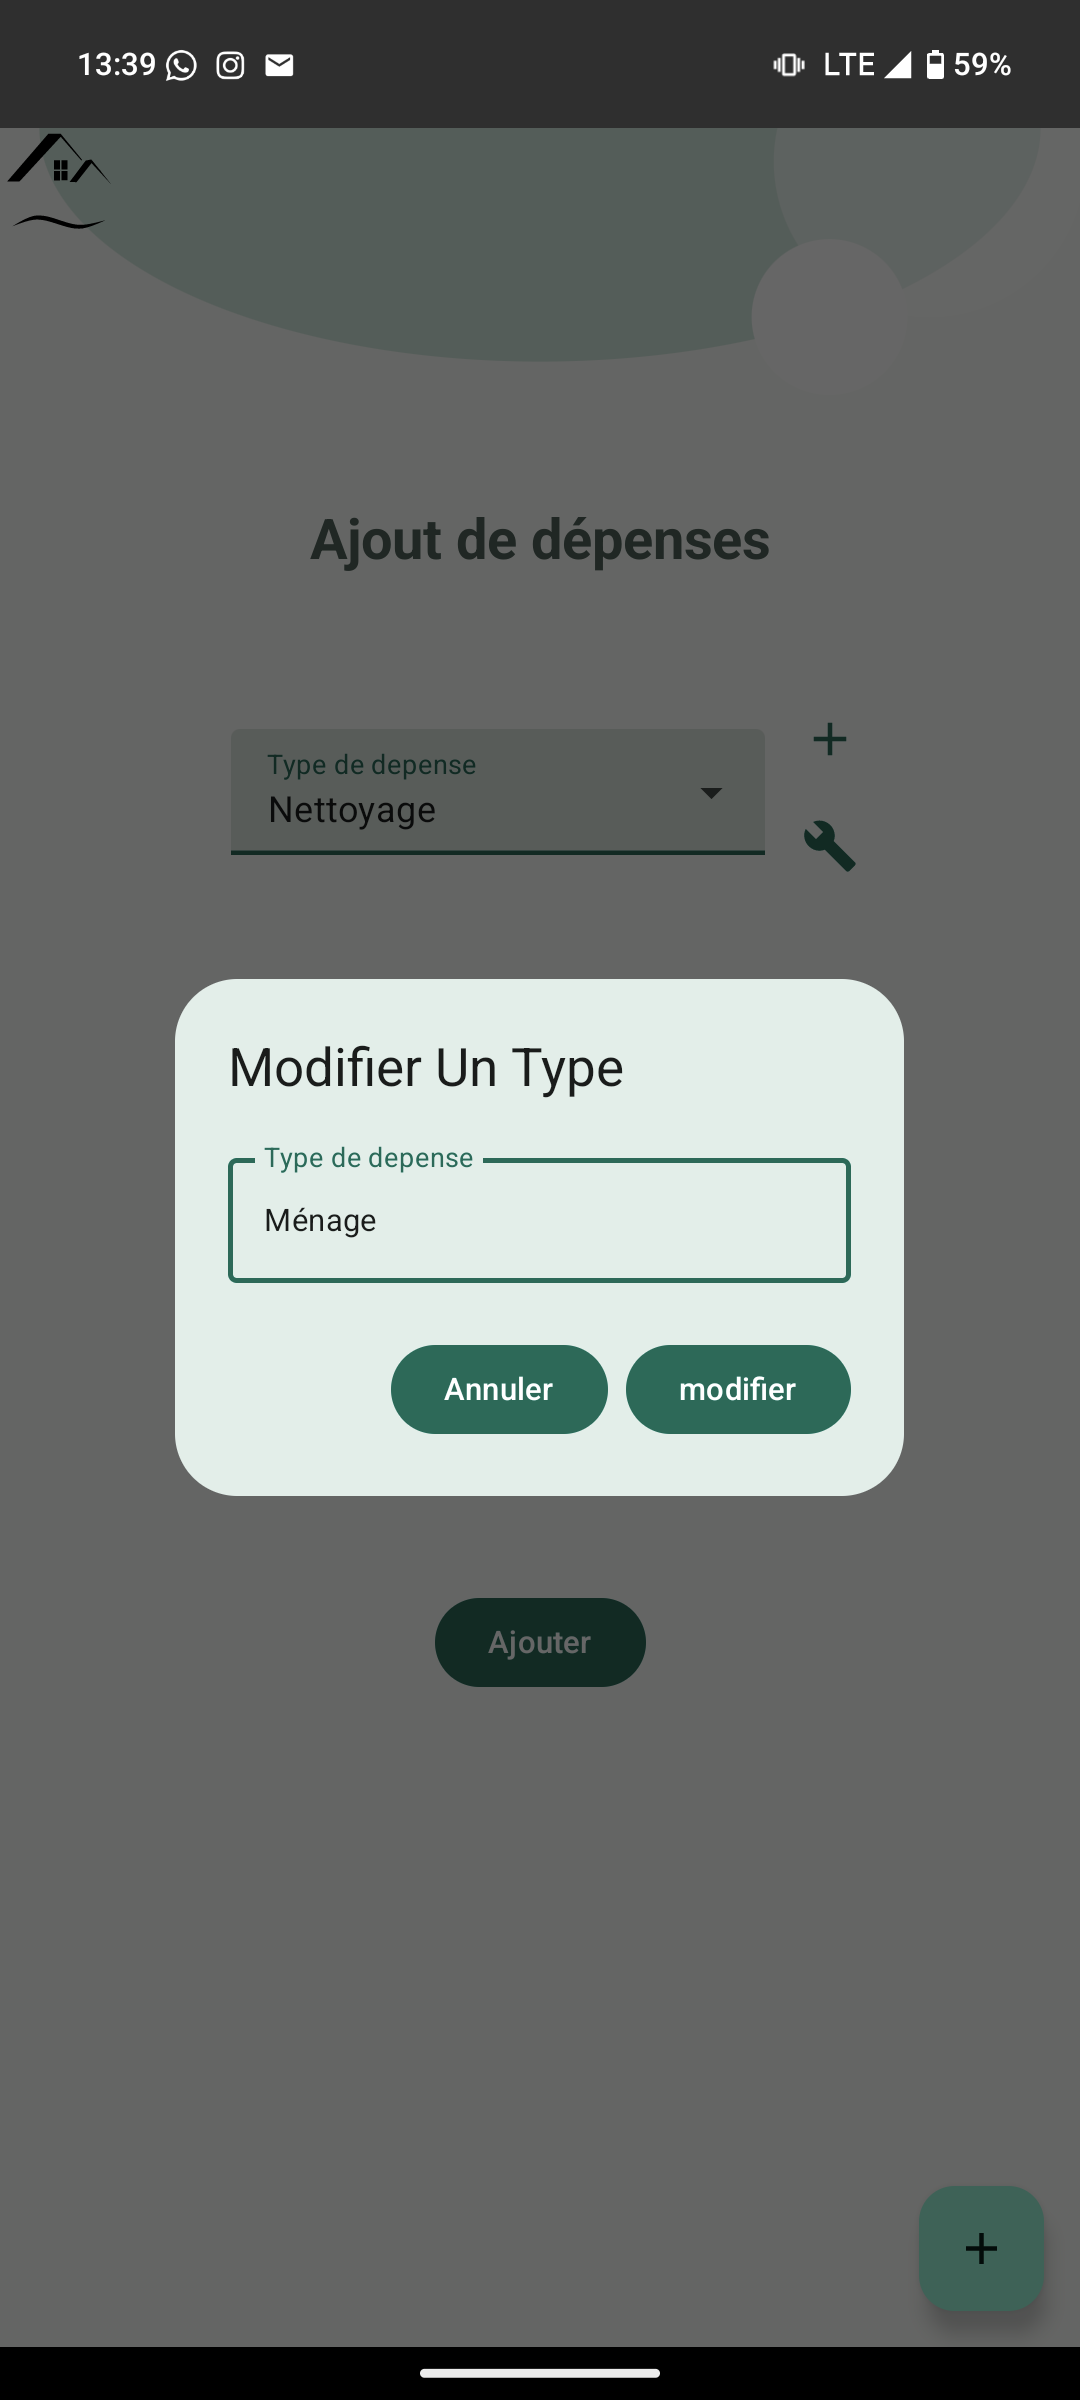
\includegraphics[width=\linewidth]{Screenshots/c4.png}
              \caption{ interface de modification d'un  type de depense}
      \end{minipage}%
        \end{figure}

      \subsubsection{ ajout de cotisation}
      \begin{figure}[!htbp]
        \begin{minipage}[t]{0.4\textwidth}    %% b or t, default is c
                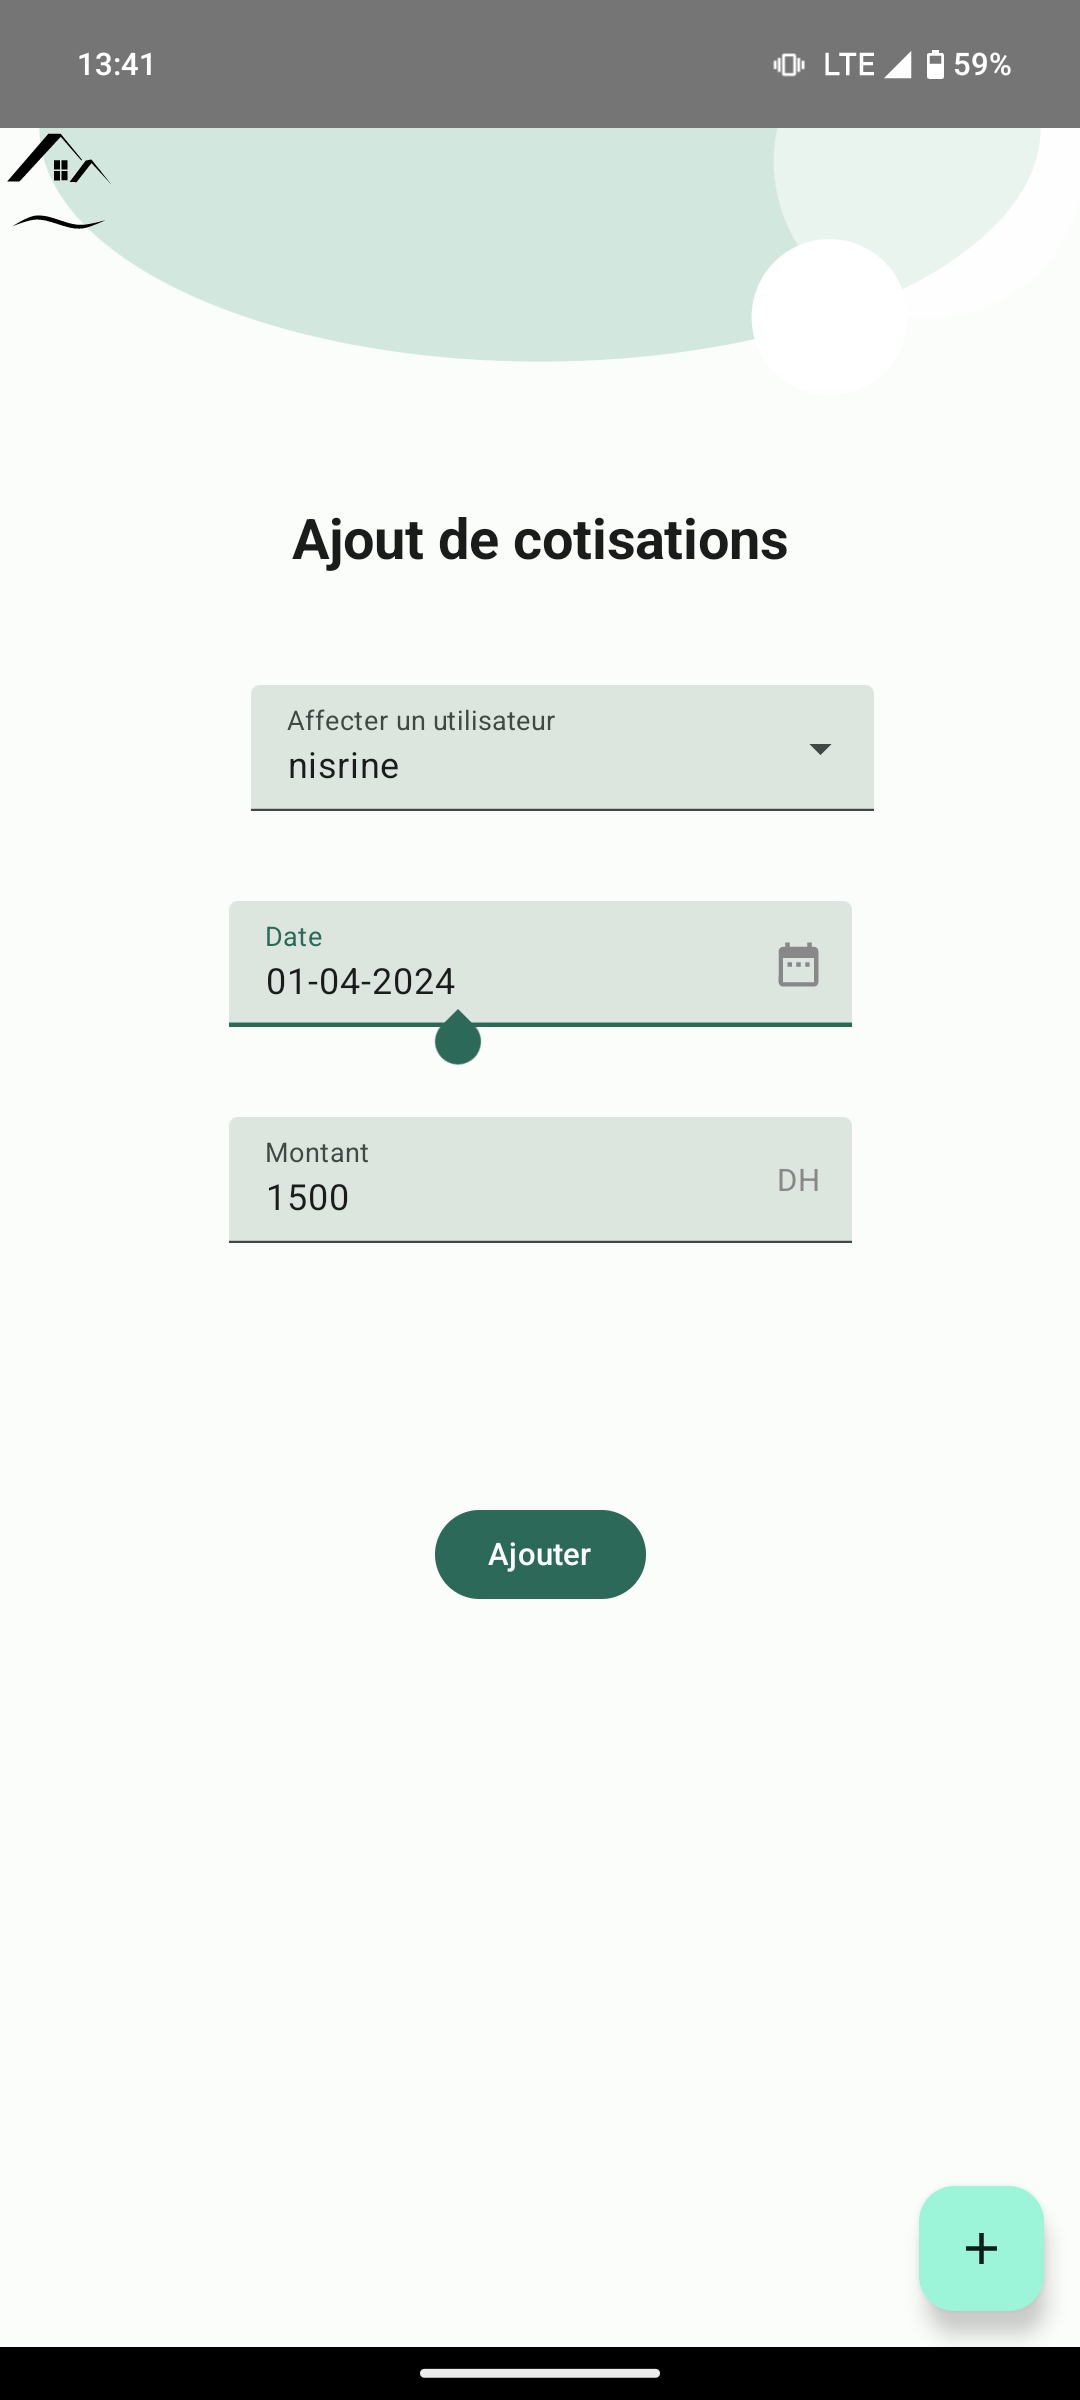
\includegraphics[width=\linewidth]{Screenshots/c8.png}
                \caption{ exemple d'interface pour ajouter des cotisation}
        \end{minipage}%
        \begin{minipage}{0.20\textwidth}
          \hfill
        \end{minipage}
      \begin{minipage}[t]{0.4\textwidth}
              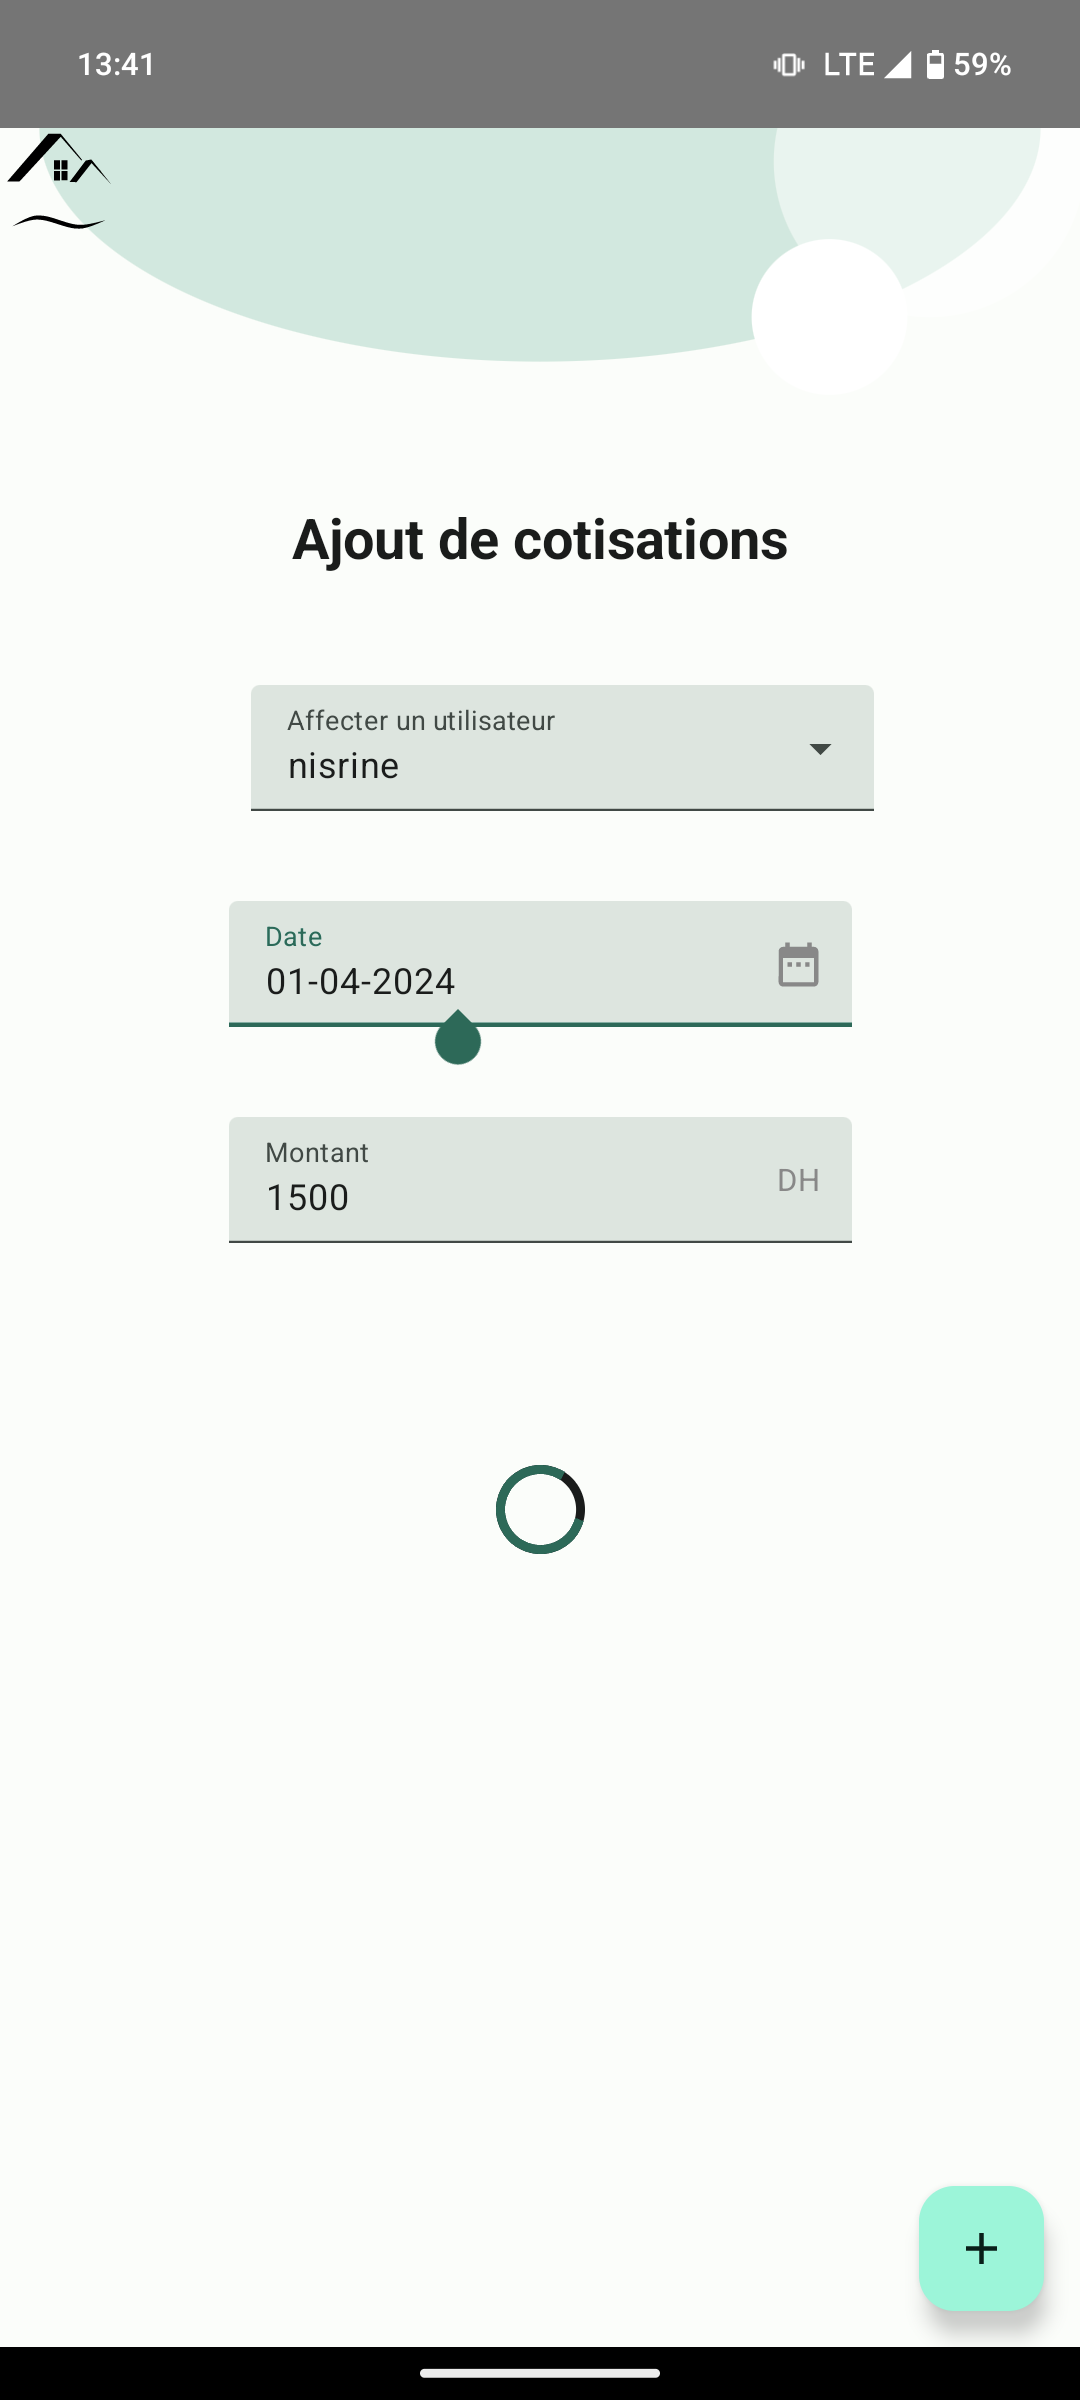
\includegraphics[width=\linewidth]{Screenshots/c9.png}
              \caption{ exemple d'opération en cours ( ajout de cotisation)}
      \end{minipage}%
        \end{figure}
        \begin{figure}[!htbp]
          \begin{minipage}[t]{0.4\textwidth}    %% b or t, default is c
                  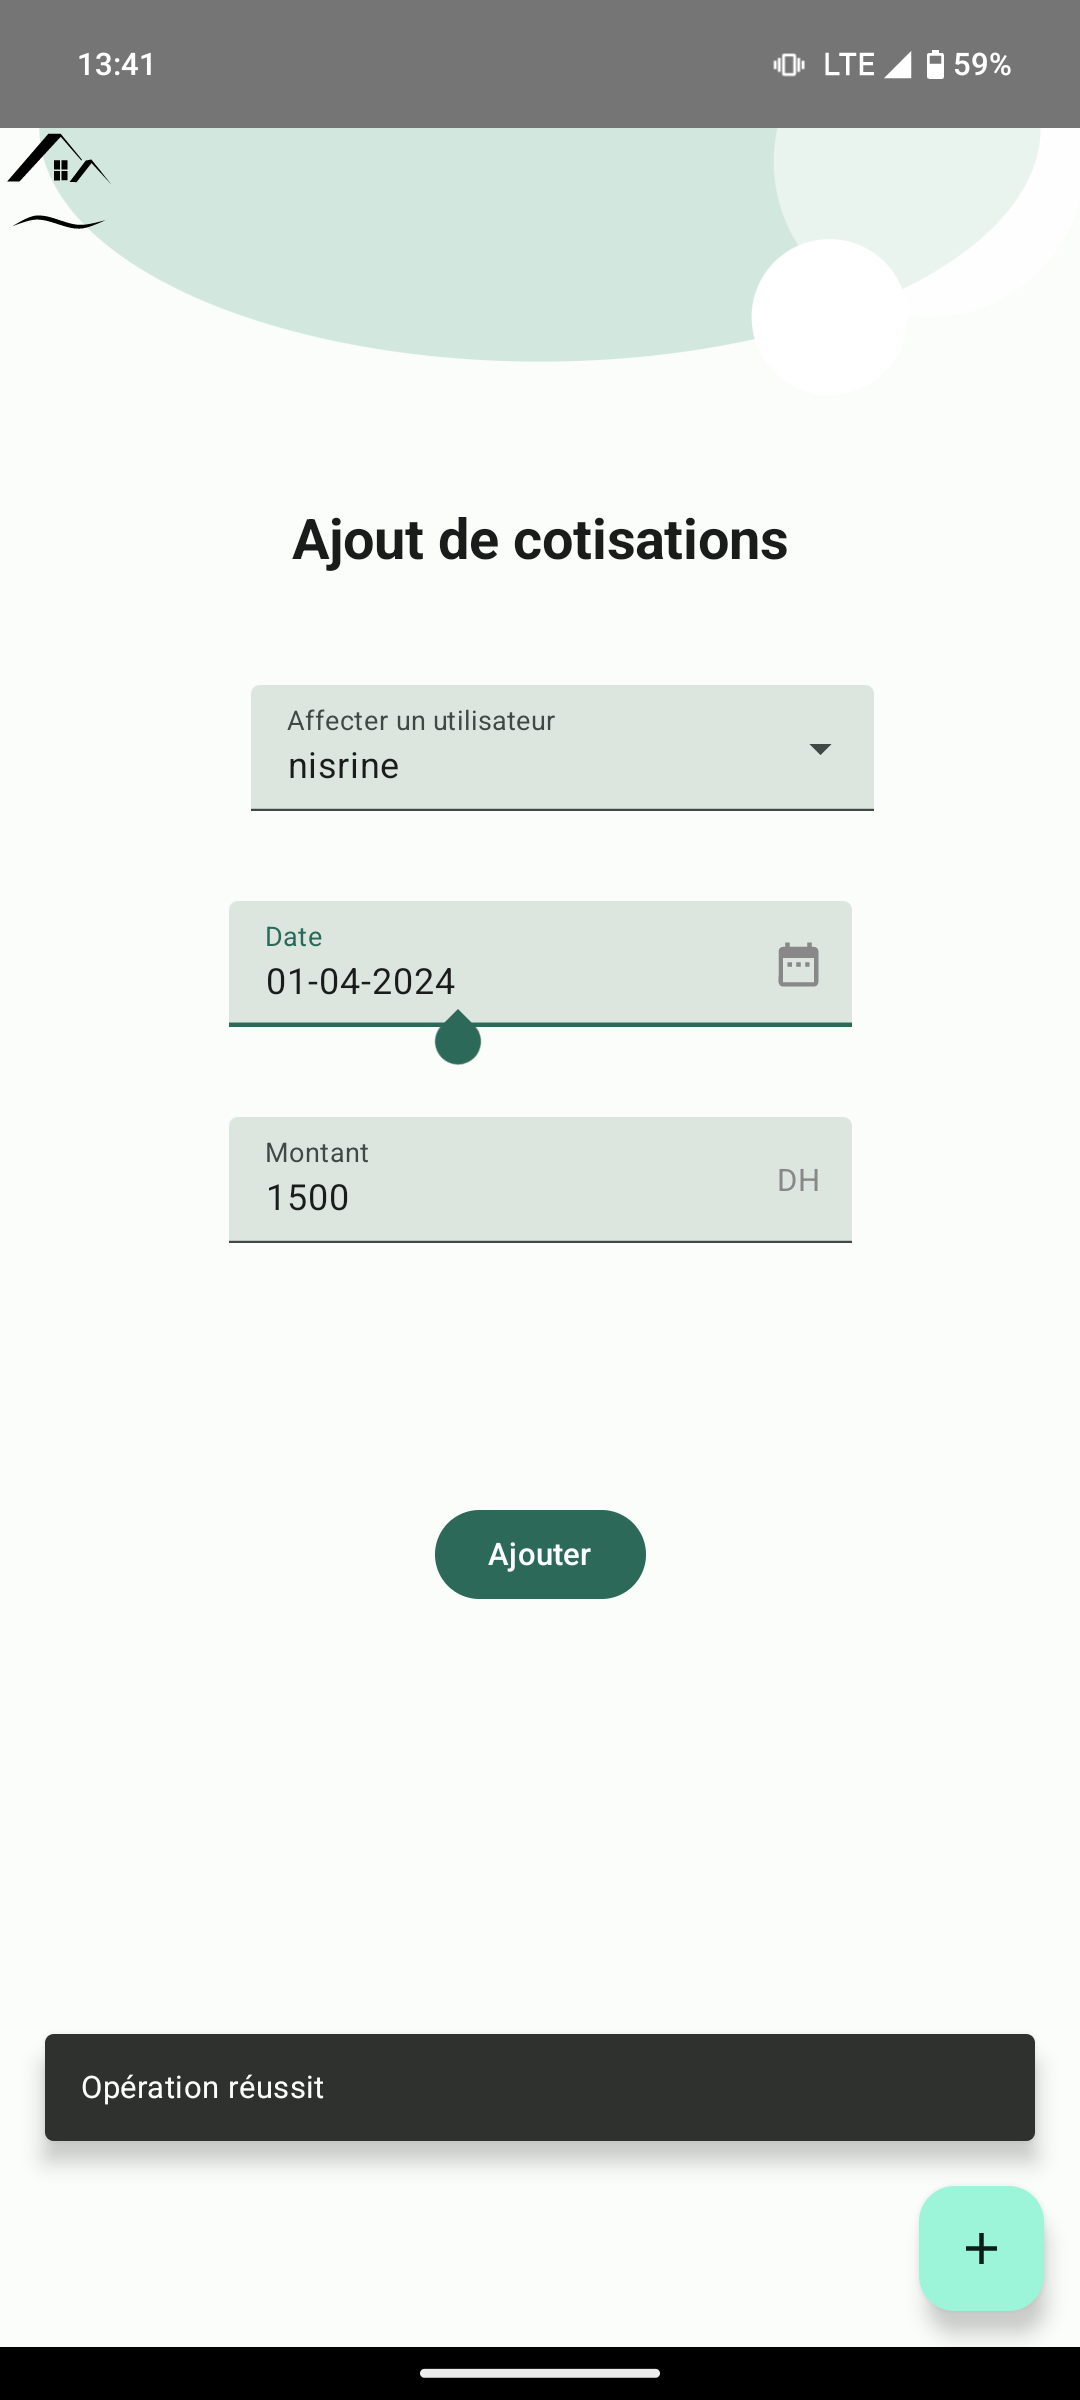
\includegraphics[width=\linewidth]{Screenshots/c10.png}
                  \caption{ exemple de message de reussit d'ajout de cotisation}
          \end{minipage}%
          \end{figure}


  \subsubsection{suppression des operations}
  \begin{figure}[!htbp]
    \begin{minipage}[t]{0.4\textwidth}    %% b or t, default is c
            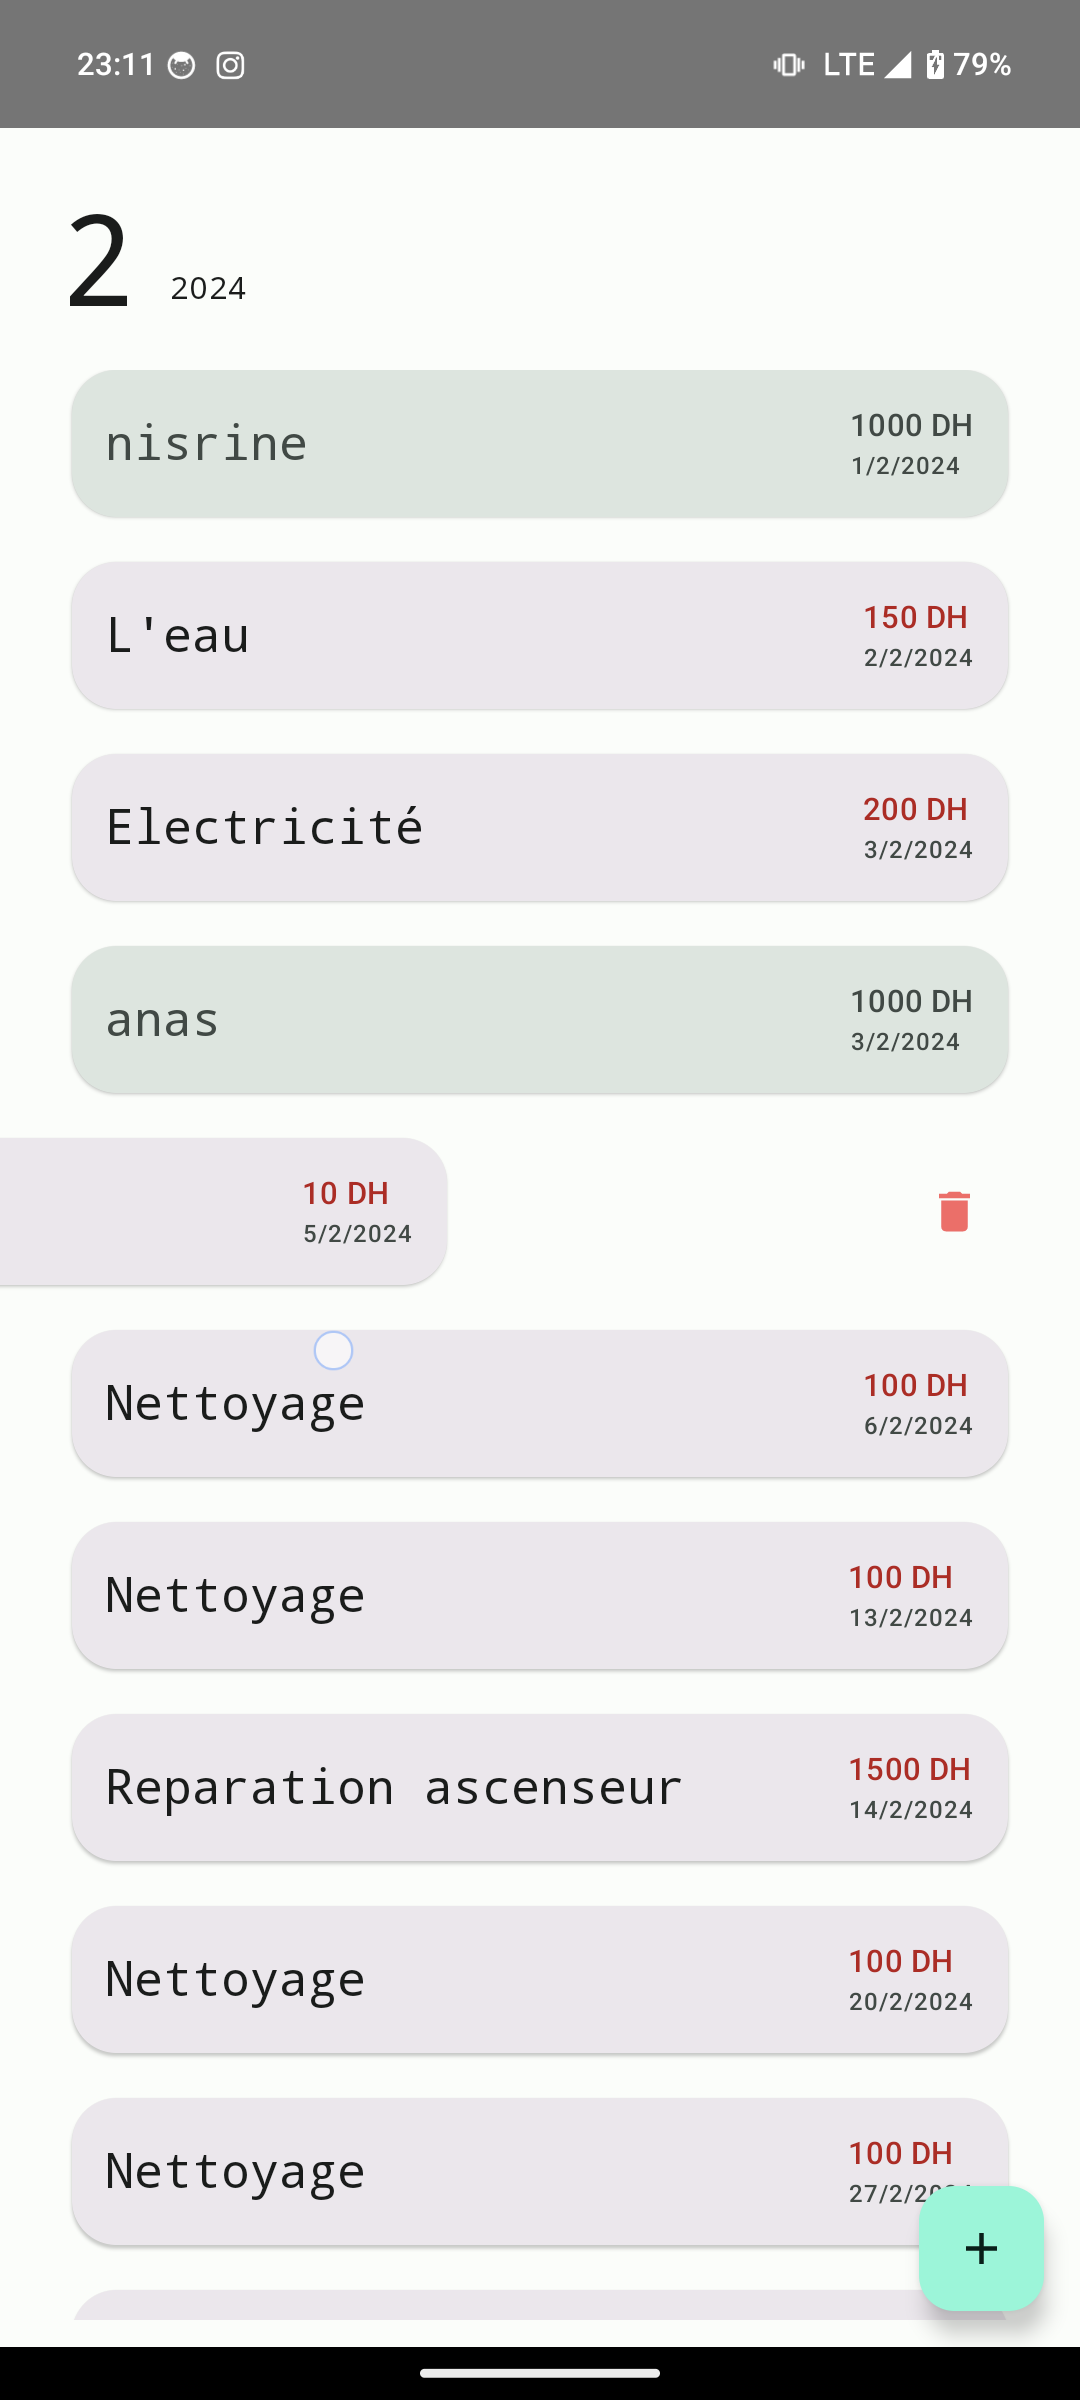
\includegraphics[width=\linewidth]{Screenshots/3.png}
            \caption{ exemple de suppression d'une operation par l'administrateur}
    \end{minipage}%
    \begin{minipage}{0.20\textwidth}
      \hfill
    \end{minipage}
  \begin{minipage}[t]{0.4\textwidth}
          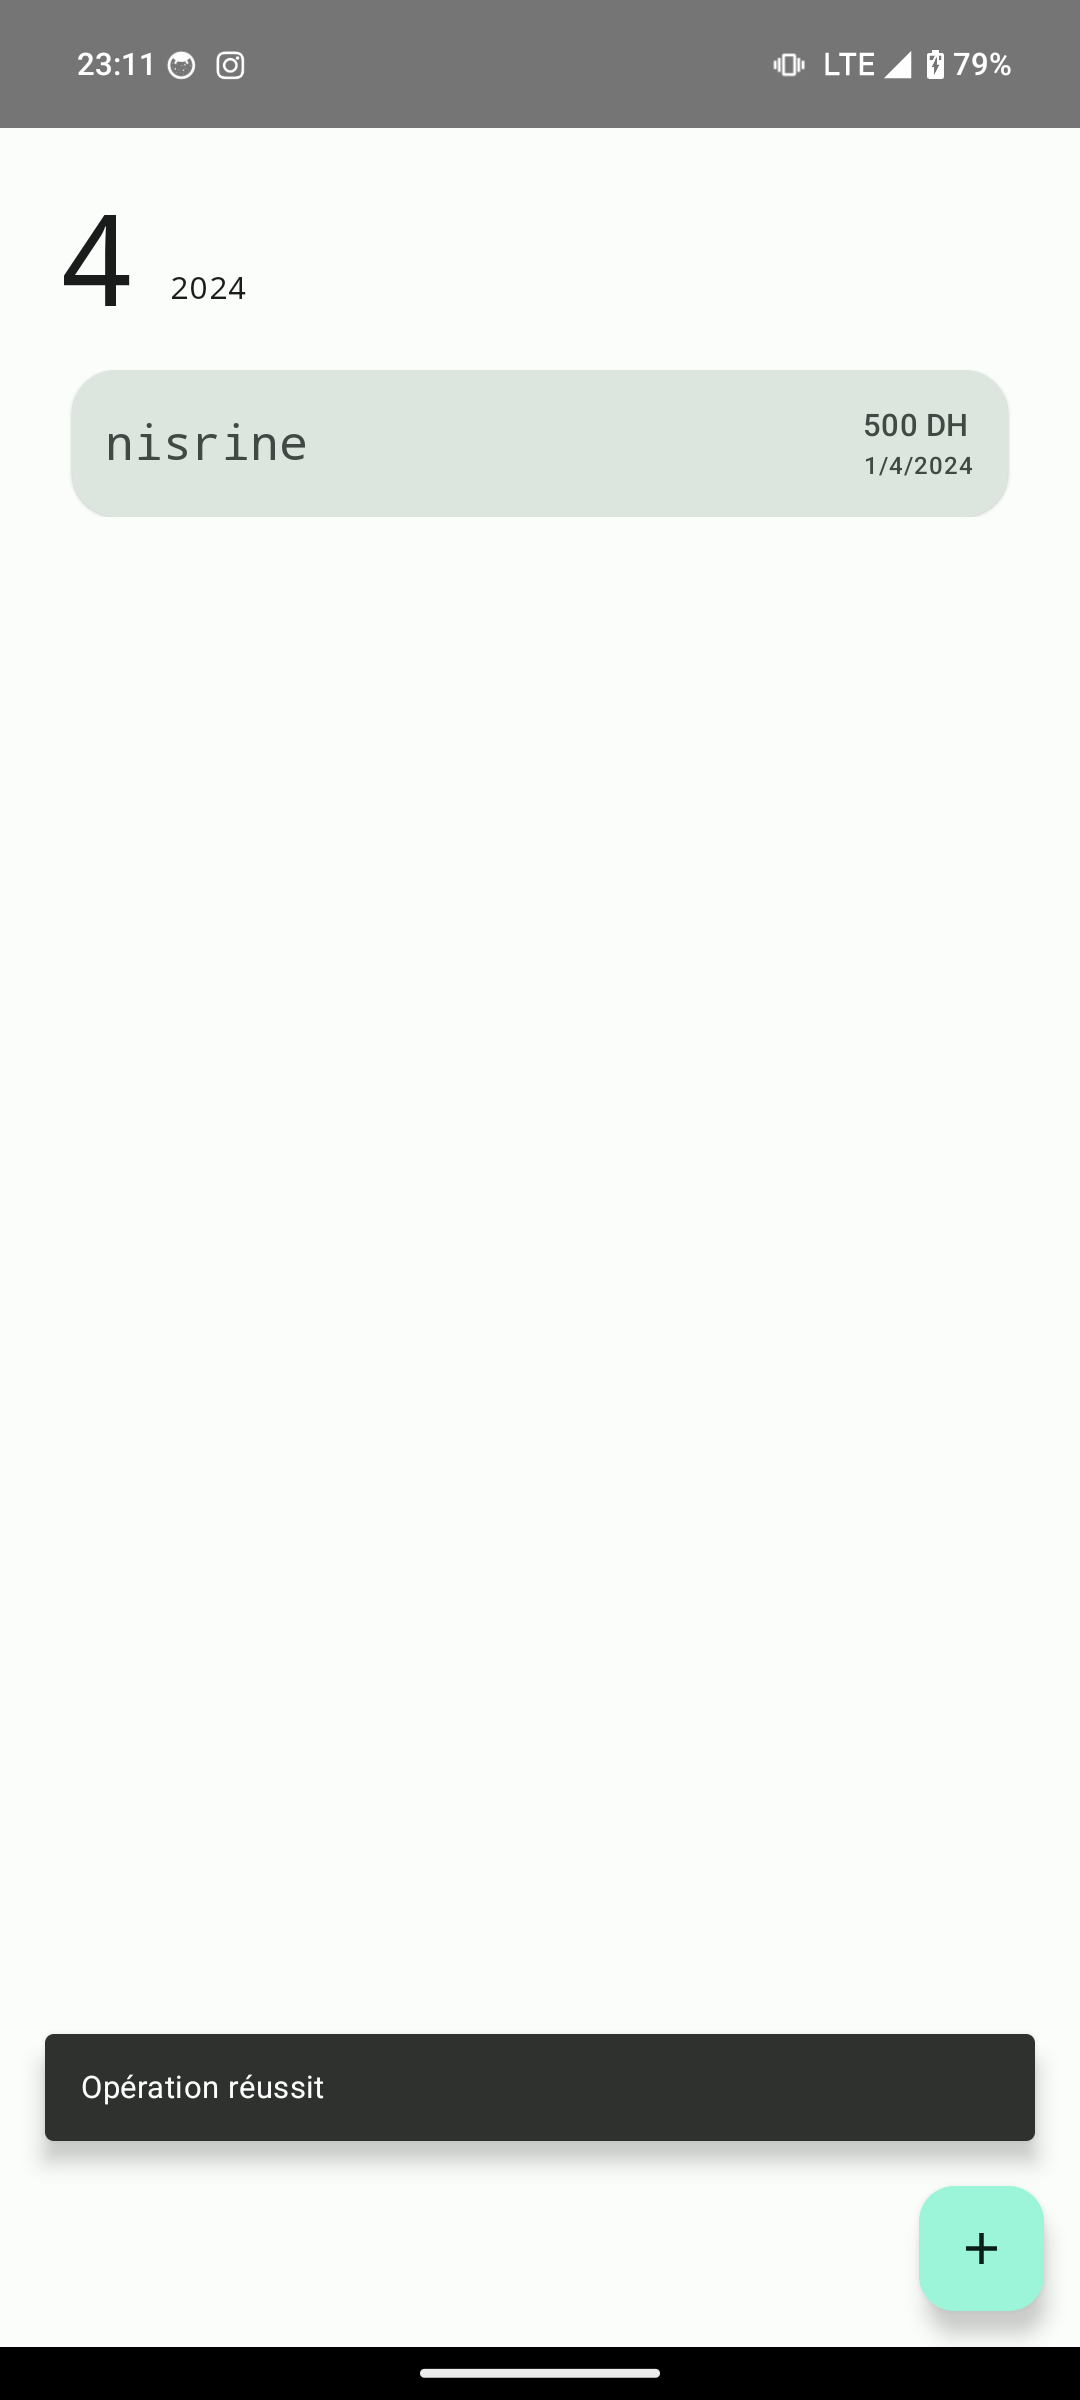
\includegraphics[width=\linewidth]{Screenshots/5.png}
          \caption{ message de reussit}
  \end{minipage}%
    \end{figure}


